\documentclass[a4paper,fleqn]{cas-sc}
\RequirePackage{fix-cm}

\usepackage[authoryear,longnamesfirst]{natbib}
\usepackage{amsmath,amssymb,amsfonts}
\usepackage{graphicx}
\graphicspath{{../Images/}{../policy_figures/}}
\usepackage{booktabs}
\usepackage{color}
\usepackage{float}
\usepackage{enumitem}
\usepackage{caption}
\usepackage{fancyhdr}
\usepackage{subcaption}
\usepackage{xcolor}
\usepackage{array}
\usepackage{tabularx}
\usepackage{multirow}
\usepackage{setspace}
\usepackage{pgfplots} 
\pgfplotsset{compat=1.18}
\usepackage{algorithm} 
\usepackage{algpseudocode}
\usetikzlibrary{positioning}
\usepackage{listings}
\usepackage{pdflscape}
\usepackage{tikz}
\usetikzlibrary{positioning, shapes.geometric}
\usepackage{changepage}
\usepackage{adjustbox}
\usepackage{hyperref}

%%%Author macros
\def\tsc#1{\csdef{#1}{\textsc{\lowercase{#1}}\xspace}}
\tsc{WGM}
\tsc{QE}
%%%

\usepackage{lastpage}

\newcolumntype{Y}{>{\raggedright\arraybackslash}X}

% Define page style for main document (just page numbers)
\fancypagestyle{maintext}{%
  \fancyhf{}%
  \fancyfoot[C]{\thepage}%
}

% Set main document to use the simple page style
\pagestyle{maintext}

% Short author
\shortauthors{Zhao et al.}  
% Main title of the paper
\title [mode = title]{ABM-ETOP: An Agent-Based Framework for Evaluating Multimodal Subsidy Allocation\\Policies for Equity and Efficiency}  

% First author
\author[1]{Ruiyi Zhao}
% Corresponding author indication
\cormark[1]
% Footnote of the first author
\fnmark[1]
% Email id of the first author
\ead{ruiyi.zhao1@unsw.edu.au}
% URL of the first author
\ead[url]{https://rciti.unsw.edu.au/}

% Second author
\author[1]{Taha Rashidi}
% Footnote of the second author
\fnmark[2]
% Email id of the second author
\ead{rashidi@unsw.edu.au}

% Third author with dual affiliation
\author[2,1]{S. Travis Waller}
% Footnote of the third author
\fnmark[2]
% Email ids of the third author
\ead{s.waller@unsw.edu.au}
\ead{steven_travis.waller@tu-dresden.de}


% Define the two unique affiliations
\affiliation[1]{organization={Research Centre for Integrated Transport Innovation (rCITI), School of Civil and Environmental Engineering, UNSW},
            city={Sydney},
            postcode={2052}, 
            state={NSW},
            country={Australia}}

\affiliation[2]{organization={"Friedrich List" Faculty of Transport and Traffic Sciences, Technische Universität Dresden},
            addressline={Professor and Chair of Transport Modelling and Simulation}, 
            city={Dresden},
            country={Germany}}


\begin{document}

\begin{abstract}
ABM-ETOP is an agent-based framework for evaluating budget-constrained transport subsidy allocation policies under heterogeneous traveller behaviour, provider responses, and network feedback. The present revision focuses on fixed-pool subsidy (FPS) levels and percentage-based subsidy allocations across subsidizable MaaS, shared-mobility, public-transport, and walking options. Rather than a single multi-objective optimizer, the workflow uses three separate single-objective Bayesian optimisation runs for mode-share equity, travel-time equity, and total system travel time, followed by a cross-policy synthesis.

The revised evidence base is seed-based. For each sampled FPS value, candidate policies are re-evaluated over 30 stochastic seeds and reported with means and 95\% confidence intervals. The best seed-mean outcomes occur at FPS 7,500 for mode-share equity (mean 0.3984, 95\% CI $\pm$ 0.0276), FPS 6,500 for travel-time equity (mean 5.4794, 95\% CI $\pm$ 1.2789), and FPS 7,500 for total system travel time (7,483.23 minutes, 95\% CI $\pm$ 140.75). A regenerated cross-policy comparison identifies FPS 7,500 as the strongest common compromise among the shared sampled FPS values. At the objective-specific optima, the largest aggregate allocation share goes to low-income travellers in all three cases, but because the audited optimisation bounds are 0.0--0.8 for every income-mode cell, we interpret this as an observed outcome of the revised experiments rather than as a pattern imposed by progressive bounds.

The stochastic objective curves remain irregular, which is expected in a highly stochastic ABM with random trip generation and evolving congestion. To interpret this behaviour, we add a deterministic fixed-policy control experiment that holds commuters, trip requests, and background conditions fixed across FPS values. Under that control, the FPS-response relationship becomes monotonic or near-monotonic until subsidy saturation, supporting the interpretation that the stochastic irregularity arises from the simulated system's randomness rather than from invalid optimisation logic. We therefore position ABM-ETOP as a reproducible scenario-analysis framework for subsidy allocation, while leaving city-scale monetised benefit claims for future work with a verified mapping from model units to real-world costs.
\end{abstract}


\begin{keywords}
transport equity \sep agent-based modeling \sep subsidy optimisation \sep Bayesian optimisation \sep evidence-based policy
\end{keywords}

\maketitle

\section{Introduction}\label{sec:intro}
Transport systems connect people to employment, education, health care, and social activity, but they also reproduce inequities and inefficiencies. Low-income households often face longer travel times, narrower modal options, and higher travel costs relative to income \citep{Lucas2016, Allen2019}. Congestion and poorly targeted subsidies can compound those burdens while also degrading overall system performance \citep{AFTABUZZAMAN20101}. Transport subsidies are therefore a central policy instrument, yet their effects depend on behavioural heterogeneity, provider responses, and budget constraints that are difficult to capture in static planning tools \citep{Pereira2017, Martens2017b, ITF2024}. As \citet{Martens2016} argues, transport policy design matters because inequity can persist even when resources are substantial but poorly targeted.

This paper presents the Agent-Based Model for Equity-Transport Optimisation and Policy (ABM-ETOP) as a subsidy-allocation evaluation framework rather than a general transport-policy optimiser. The framework combines an agent-based simulation with Bayesian optimisation to study fixed-pool subsidy levels and percentage-based allocations across subsidizable modes. In the current implementation, the model covers public transport, shared car services, shared bike services, MaaS bundles, and walking. Privately owned cars and private bikes are not included because the policy instrument analysed here is an operating subsidy delivered through the MaaS platform rather than an ownership, parking, or fuel policy.

The revision reported here is driven by a new evidence pipeline. Earlier single-run claims have been replaced by repeated-seed summaries, 95\% confidence intervals, and a deterministic fixed-policy control experiment. Section \ref{sec:lit} reviews transport-equity and subsidy-modelling gaps. Section \ref{sec:framework} describes the ABM-ETOP architecture, scope, and metrics. Section \ref{sec:optimisation} clarifies the single-objective Bayesian optimisation workflow, stochastic repetition, and reproducibility design. Sections \ref{sec:results} and \ref{sec:synthesis} present the updated seed-based results and cross-policy interpretation. Section \ref{sec:implications} draws scenario-specific policy lessons and states the limits of the current evidence, and Section \ref{sec:conclusions} summarises the contribution and future work.

\section{Literature Review and Research Gaps}\label{sec:lit}

\subsection{Transport Equity Frameworks}
Transport equity concerns the fair distribution of mobility opportunities, burdens, and benefits. Horizontal equity typically refers to equal treatment among similarly situated travellers, whereas vertical equity focuses on outcomes for disadvantaged groups such as low-income households \citep{Litman2025, vanWee2011}. In practice, the two perspectives do not map cleanly onto any single transport-performance indicator, which is why this paper reports two equity-focused outcomes and one separate system-efficiency outcome rather than claiming that one metric fully represents all equity dimensions. The policy challenge is well documented: public transport and mobility investments often miss the households most affected by transport disadvantage \citep{Allen2019, Titheridge2014, Lucas2012}. ABM-ETOP is intended as a scenario-analysis framework that helps evaluate how different subsidy allocations distribute gains and burdens across traveller groups under those competing concerns.

\subsection{Critical Assessment of Existing Modeling Approaches}\label{sec:model_critique}

Providing transport subsidies is one policy lever for improving transport equity \citep{Lucas2016}. We focus on two linked policy elements: fixed-pool subsidies (FPS), which cap the available budget, and percentage-based subsidies (PBS), which determine how that budget is distributed across income groups and modes. Existing tools struggle when the analysis requires heterogeneous traveller responses, provider behaviour, and explicit optimisation over a subsidy-allocation matrix. This section therefore reviews four-step models, activity-based models, and other transport ABMs with a specific emphasis on their suitability for FPS and PBS analysis before positioning ABM-ETOP as a tailored scenario-analysis framework.

\subsubsection{Four-Step Transport Models}
Four-step models have been the backbone of transport planning since the 1950s. It includes trip generation, distribution, mode choice, and traffic assignment \citep{McNally2007a}. Their strengths include simplicity and basic socio-economic data (e.g., population, employment) requirements. It is eminently effectiveness for aggregate planning, such as estimating total trip volumes \citep{McNally2007a}. However, their reliance on aggregated regional data hides the crucial individual behaviours needed for equity analysis \citep{Martens2006}. Their static, sequential structure assumes fixed relationships, ignoring dynamic feedback (e.g., how subsidy distributions affect mode choice behaviour among diverse socioeconomic traveller segments) \citep{McNally2007a}. They lack the preciseness to model income-based subsidy impacts or optimise FPS budgets, making them inadequate for equity-focused FPS and PBS evaluation, as they cannot assess distributional effects across diverse groups \citep{Zhao2016}.

\subsubsection{Activity-Based Models}
Activity-based models are powerful transport planning and travel-demand forecasting tools. They simulate individual travellers' daily activities and travel decisions, capturing behavioural heterogeneity and dynamic interactions \citep{McNally2007b}. Their strengths include behavioural realism, policy sensitivity, and the ability to represent differential impacts across groups \citep{McNally2007b}. However, they also face familiar challenges: large data requirements, computational intensity, and the need for substantial model customisation when policy instruments depart from standard demand-management settings \citep{Freedman2025}. Two well-known examples are:

\begin{itemize}
    \item \textbf{MATSim}: MATSim is an open-source activity-based modelling framework well suited to large-scale simulations and detailed temporal modelling of individual mode and route choices \citep{Horni2016}. Its use in public-transport network design demonstrates clear relevance for subsidy analysis, but detailed income-based heterogeneity and percentage-based subsidy matrices typically require custom extensions and additional data integration \citep{Jafari2024}. Its computational demands and the need for custom MaaS/provider logic also complicate direct FPS/PBS optimisation.
    \item \textbf{POLARIS}: POLARIS, developed by Argonne National Laboratory, simulates interactions among travellers, vehicles, and providers \citep{Auld2016}. It supports policy analysis, including subsidy experiments, but its simulation-oriented design still requires additional optimisation logic for explicit FPS/PBS search and detailed subsidy-allocation constraints \citep{Wong2020}.
\end{itemize}

\subsubsection{Other Agent-Based Models}
Other ABMs, often custom-built or commercial, are tailored to tasks such as traffic operations, infrastructure analysis, or narrowly defined policy studies \citep{Bazzan2014}. Their diversity is useful, but it also means that modelling choices, data structures, and validation practice can vary substantially \citep{Kagho2020}. Many face the same computational and data challenges as activity-based models and do not include an optimisation layer designed for structured FPS/PBS policy search \citep{Zhao2016}.

\subsubsection{The ABM-ETOP Framework}
ABM-ETOP addresses these gaps with a hybrid multi-agent system tailored to FPS and PBS analysis. It combines agent-based behavioural heterogeneity with Bayesian optimisation, allowing the study to search over subsidy-allocation matrices while preserving dynamic provider responses and network feedback. Table \ref{tab:model_comparison} is intended as a conceptual capability comparison rather than as an empirical benchmarking exercise. On that basis, ABM-ETOP contributes a focused environment for subsidy-allocation experiments that are difficult to run in more general transport planning tools without substantial customisation.

ABM-ETOP also makes deliberate simplifications. The current implementation uses a stylised grid environment rather than a full city network, simplified commuter utility rules, and a relatively small synthetic population. The optimisation study reported here runs on a 100$\times$100 grid with 200 commuters, while some visualisation exports use smaller debugging grids for readability. These choices make repeated-seed policy evaluation computationally tractable, but they also limit direct transfer to real-world network design or city-scale deployment without further calibration and network integration \citep{Horni2016, Auld2016, Axhausen2010}.

\begin{table}[!t]
\caption{Comparison of Transport Modeling Approaches for FPS and PBS Analysis}
\label{tab:model_comparison}
\centering
\begin{tabular}{lcccc}
\toprule
\textbf{Model Type} & \textbf{Heterogeneity}& \textbf{Dynamic Feedback} & \textbf{Subsidy Optimisation}& \textbf{Provider Dynamics} \\
\midrule
Four-Step & No & No & No & No \\
Activity-Based Models & Yes& Limited & Limited& Limited \\
Other Agent-Based Models & Limited & Yes & Limited & Limited \\
\textbf{ABM-ETOP (this study)} & Yes & Yes & Yes & Yes \\
\bottomrule
\end{tabular}
\footnotesize
\texttt{Note: Comparison focuses on capabilities for FPS and PBS analysis. ABM-ETOP employs spatial and behavioural simplifications compared to established ABMs' comprehensive transport modelling capabilities.}
\end{table}

\section{The ABM-ETOP Framework: Conceptual Overview}\label{sec:framework}

\subsection{Framework Architecture and Core Innovations}

This section presents the architecture and formal representation of the ABM-ETOP framework. As Figure~\ref{fig:overall_framework_architecture} illustrates, the framework integrates agent-based simulation and Bayesian optimisation to evaluate subsidy-allocation strategies across multiple policy criteria.
\begin{figure}[t]
    \centering
    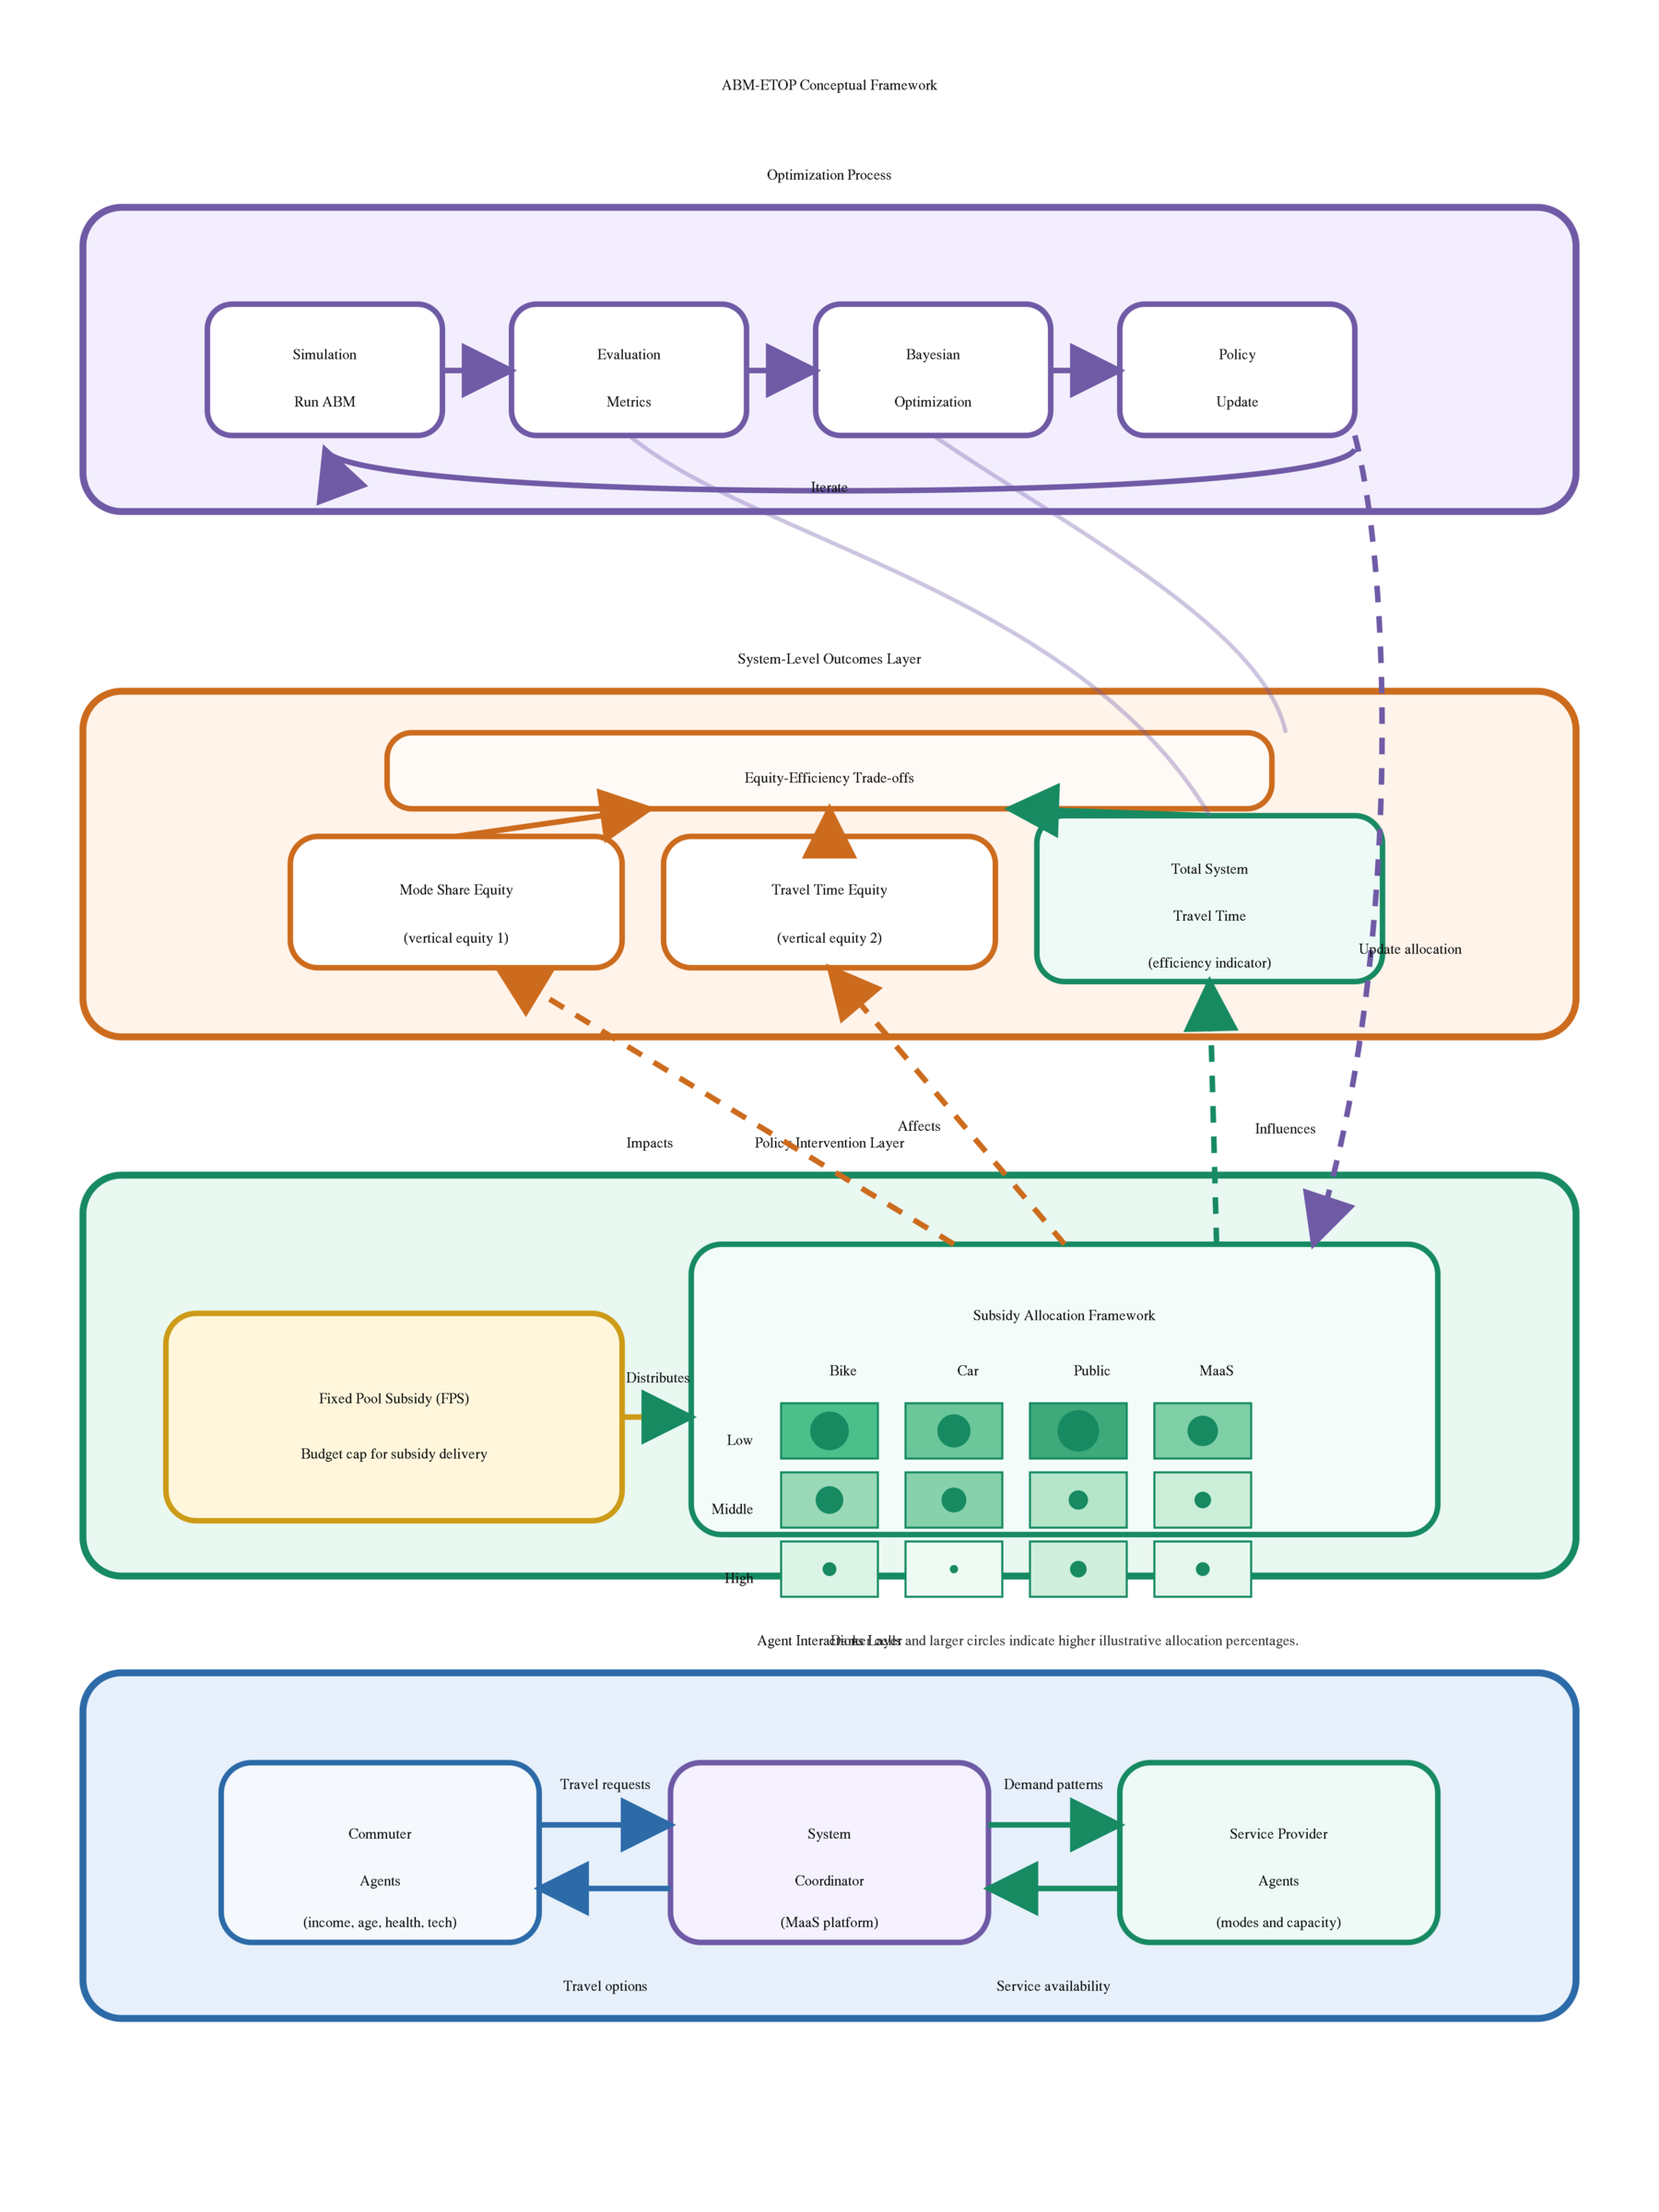
\includegraphics[width=0.9\textwidth]{1_abm_etop_framework_fixed.png}
    \caption{ABM-ETOP framework architecture showing the integration of agent-based modeling with Bayesian optimisation for policy evaluation. The framework consists of four interacting layers: agent interactions, policy interventions, system-level outcomes, and optimisation processes. In the policy-allocation inset, darker cells and larger circles denote higher illustrative allocation percentages.}
    \label{fig:overall_framework_architecture}
\end{figure}

At the core of the ABM-ETOP framework lies a centralised agent-based architecture consisting of unique decision-making processes of three distinct agent types, as illustrated in Figure~\ref{fig:centralised_abm}: \textit{commuters}, \textit{service providers}, and \textit{MaaS agent}. \textit{Commuter agents} represent the individual travellers in the real world. They are differentiated by factors such as income level, value of time, and travel preferences. This differentiation is critical for understanding equity implications, as it enables a realistic representation of varied transport experiences across population segments and highlights how transport disadvantages are unevenly distributed, leading to disproportionate mobility constraints, particularly for low-income groups. The  \textit{MaaS agent} facilitates trip requests, option generation, subsidy application, and booking coordination across modes. The \textit{transport provider} agents represent different travel options, including car-share, bike-share and public transport. Each transport provider also dynamically updates their availability, pricing, and capacity based on evolving demand, competitive pressures, and policy interventions. By capturing these dynamic adaptations, the framework generates more realistic projections of how transport systems evolve in response to policy changes and evaluates the resulting distributional outcomes.

The optimisation layer searches for promising subsidy-allocation strategies without exhaustively simulating every possible combination. That substantially reduces computation while retaining the agent-based model's behavioural richness. The framework reports two equity-focused outcomes, mode-share equity and travel-time equity, alongside one system-efficiency outcome, total system travel time. We use this combination to study how subsidy allocations redistribute access, temporal burdens, and aggregate travel time without claiming that any one of the three metrics fully captures the entire equity concept.

\subsection{Formal Representation of the ABM-ETOP Framework}\label{sec:simpleformula}

To enhance conceptual clarity and establish formal parameters, this complex ABM-ETOP framework can be expressed as an transformation function:

\begin{equation}
\text{ABM-ETOP}(\mathbf{S}, \mathbf{P}, \mathbf{A}, \mathbf{E}) \rightarrow \mathbf{Y}
\end{equation}

The ABM-ETOP framework takes four strategically categorised parameter vectors as input. These are system parameters $\mathbf{S}$, which define behavioural mechanics like user sensitivity and value of time, and network characteristics; policy parameters $\mathbf{P}$, capturing intervention mechanisms, specifically the fixed pool subsidy amount and its allocation—the primary focus for optimisation; agent parameters $\mathbf{A}$, representing diverse stakeholders including heterogeneous commuters, service providers, and MaaS platform specifications; and environment parameters $\mathbf{E}$, establishing the spatiotemporal context of the network, activities, and demand. The detailed definition for each parameter class is provided in Appendix~\ref{app:param_specs} with comprehensive examples. 
Through a systematic mapping process, the framework uses these inputs to generate an output vector $\mathbf{Y}$ containing three complementary performance metrics:

\begin{equation}
\mathbf{Y} = \begin{bmatrix} E_{\text{mode}} \\ E_{\text{time}} \\ T_{\text{total}} \end{bmatrix}
\end{equation}
\subsubsection{Subsidy Policy Mechanisms}
The ABM-ETOP framework explicitly models two complementary subsidy approaches: Fixed Pool Subsidy (FPS) and Percentage-Based Subsidy (PBS). These mechanisms are formally represented within the policy parameters vector $\mathbf{P}$:

\begin{equation}
\mathbf{P} = \begin{bmatrix} \text{FPS} \\ \mathbf{A} \end{bmatrix}
\end{equation}

The Fixed Pool Subsidy (FPS) establishes a predetermined financial allocation ($\text{FPS} \in \mathbb{R}^+$) representing the total budget available for transportation subsidies. Unlike open-ended subsidisation mechanisms, FPS operates within defined fiscal constraints, better reflecting real-world budgetary limitations faced by transportation authorities. This approach enables systematic evaluation of subsidy effectiveness across varying investment levels and facilitates direct comparison between different allocation strategies.

The Percentage-Based Subsidy (PBS) is operationalised through the allocation matrix $\mathbf{A} = \{a_{i,m}\} \in [0,1]^{I \times M}$, which specifies subsidy percentages for each combination of income group $i \in I$ and transportation mode $m \in M$. This matrix governs what proportion of the original fare cost is subsidised for each population segment across every available transportation mode, enabling sophisticated targeting strategies that can vary by both socioeconomic status and mode choice.

The allocation matrix is subject to two essential constraints. First, boundary constraints ($L_{i,m} \leq a_{i,m} \leq U_{i,m}$) establish permissible subsidy ranges for each income-mode combination, preventing practically infeasible solutions. Second, the budget constraint ensures total subsidies remain within the established FPS limit:

\begin{equation}
\sum_{i}\sum_{m}a_{i,m} \cdot C_{i,m} \cdot D_{i,m} \leq \text{FPS}
\end{equation}

Where $C_{i,m}$ represents the original cost of mode $m$ for income group $i$ and $D_{i,m}$ denotes the corresponding demand. This formulation enables the framework to model progressive subsidy strategies where disadvantaged populations receive proportionally higher support, in contrast to uniform subsidies that apply equal percentages regardless of socioeconomic status.

For a given trip by a commuter in income group $i$ using mode $m$, the effective subsidized cost $C'_{i,m}$ is calculated as:

\begin{equation}
C'_{i,m} = C_{i,m} \cdot (1 - a_{i,m})
\end{equation}

The framework's integration of FPS and PBS mechanisms facilitates comprehensive exploration of equity-efficiency trade-offs across the subsidy parameter space, supporting evidence-based calibration of transportation policy interventions.

\subsubsection{Evaluation Metrics}\label{sec:metricequations}

One of the three complementary metrics employed by the ABM-ETOP framework is the mode-share equity metric ($E_{\text{mode}}$). It measures disparities in transport mode access across income groups:

\begin{equation}
E_{\text{mode}}(\mathbf{A}) = \sum_{i}w_i \cdot \sum_{m}\varphi(|s_{i,m} - \bar{s}_{m}|)
\end{equation}

In the equation, $w_i$ represents the population weight for income group $i$, $s_{i,m}$ is the mode share of mode $m$ for income group $i$, and $\bar{s}_{m}$ is the average mode share for mode $m$ across all income groups. Function $\varphi(x)$ provides scaling so that the reported metric is dimensionless. Lower values indicate smaller mode-share disparities, with a theoretical minimum of zero under perfect equality across income groups.

The travel-time equity metric ($E_{\text{time}}$) measures whether the transport system is placing a heavier time burden on some income groups than on others:

\begin{equation}
E_{\text{time}}(\mathbf{A}) = \sum_{i}|t_i - \bar{t}|
\end{equation}

Where $t_i$ is the average travel time for income group $i$ and $\bar{t}$ is the overall average travel time across all income groups. Because the metric sums absolute deviations in mean travel time, it is reported in minutes. Lower values indicate smaller differences in average travel times between income groups, with a theoretical minimum of zero under perfect equality in temporal burdens.

The total system travel time metric ($T_{\text{total}}$) evaluates system-wide efficiency by summing all travel time accumulated by all commuters within the simulation period:

\begin{equation}
T_{\text{total}}(\mathbf{A}) = \sum_{i}\sum_{j}t_{i,j}
\end{equation}

In the equation, $t_{i,j}$ is the travel time for trip $j$ made by income group $i$. This metric is reported in minutes. Lower values indicate a more efficient transport system with reduced aggregate travel time burdens. Because it is an efficiency metric rather than a direct equity index, we do not place it on the same numeric scale as $E_{\text{mode}}$ or $E_{\text{time}}$ unless an explicit normalisation step is introduced for cross-policy comparison.

\subsection{ABM-ETOP Simulation Process and Decision Mechanisms}

\begin{figure}[!t]
\centering
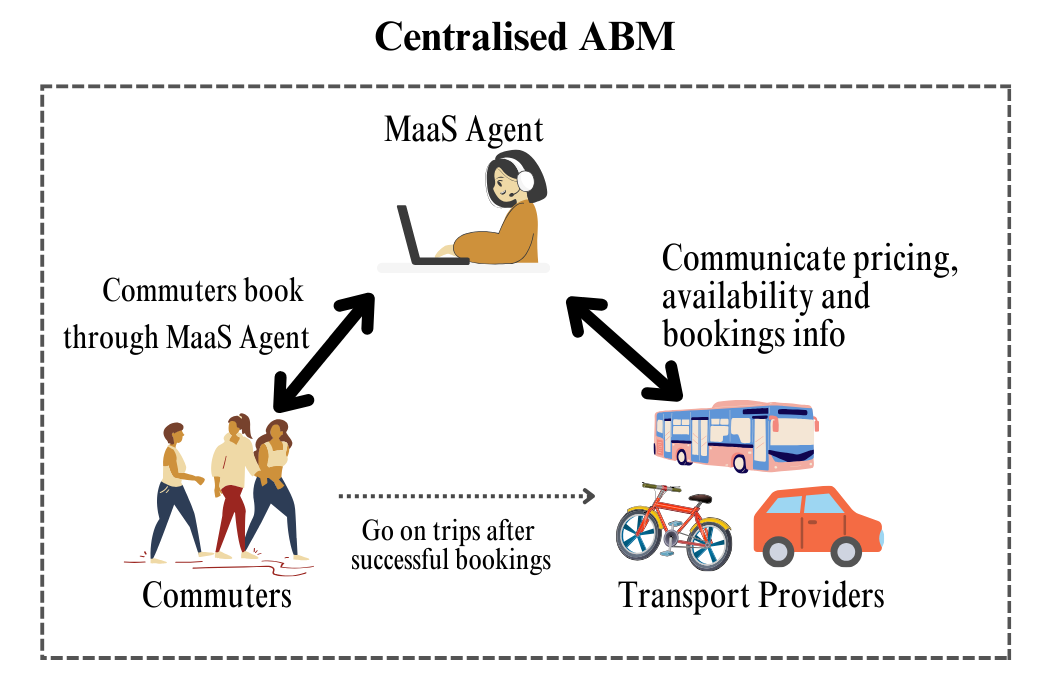
\includegraphics[width=0.8\textwidth]{2_centralised_ABM.png}
\caption{Centralised ABM-ETOP architecture showing interactions between commuter agents, the MaaS coordination agent, and transport provider agents. Commuters book through the MaaS platform, which facilitates communication with providers and processes trip requests.}
\label{fig:centralised_abm}
\end{figure}
\begin{table}[width=\textwidth]
\caption{Key Equations in the ABM}
\label{tab:key_equations}
\centering
\small
\begin{tabularx}{\textwidth}{|p{0.33\textwidth}|Y|}
\hline
\textbf{Equation} & \textbf{Description} \\
\hline
$U_{i,j} = \text{ASC}_j + \beta_C \cdot (C_{i,j} - S_{i,j}) + \beta_T \cdot \text{VOT}_i \cdot T_{i,j} + \beta_W \cdot W_{i,j} + \beta_A \cdot A_{i,j}$ & Utility function for mode choice, incorporating mode constants, cost (adjusted by subsidies), time (weighted by income-specific VOT), modal penalties, and affordability adjustments. From \texttt{calculate\_generalized\_utility} in commuter agent. \\
\hline
$P(j|i) = \frac{\exp(U_{i,j})}{\sum_{k \in M} \exp(U_{i,k})}$ & Multinomial logit model for mode choice probabilities, implemented in \texttt{calculate\_mode\_choice\_probabilities} function. \\
\hline
$\text{VOT}_i = \text{VOT}_{\text{base},i} \cdot f_{\text{flexibility}}$ & Value of time calculation adjusted by trip flexibility from \texttt{get\_value\_of\_time} function. Values range from \$5 (low income) to \$20 (high income) per hour (base values, adjusted by flexibility factors). \\
\hline
$P_{\text{dynamic}} = P_{\text{base}} \cdot (1 + \alpha \cdot (DRC - DRC_{\text{base}}) \cdot (1 + \text{Demand}_{\text{change}}))$ & Dynamic pricing algorithm from \texttt{dynamic\_pricing\_share} in service provider agent, with $DRC$ as demand-to-capacity ratio. \\
\hline
$T_{\text{congested}} = T_{\text{free\_flow}} \times (1 + \alpha \times (\frac{V_{ij}}{C_{ij}})^{\beta})$ & BPR function for congestion modelling in \texttt{calculate\_congested\_travel\_time}, with parameters $\alpha=0.03$ and $\beta=1.5$. \\
\hline
$S_{i,j} = a_{c_i,m_j} \cdot C_{i,j}$ & Subsidy calculation based on income group $c_i$ and mode $m_j$, where $a_{c_i,m_j}$ is the subsidy percentage from the allocation matrix. Implemented in subsidy application mechanism. \\
\hline
\(
\text{subsidy\_available} =
\begin{cases}
\text{True}, & \text{if weekday and pool funds remain} \\
\text{False}, & \text{otherwise}
\end{cases}$ & Subsidy availability logic from \texttt{is\_subsidy\_available} in subsidy pool agent, restricting subsidies to weekdays with remaining pool funds. \\
\hline
\end{tabularx}
\end{table}

\begin{table}[width=\textwidth]
\caption{Algorithm 1 ABM-ETOP Simulation}
\label{alg:abm-etop}
\hrule height 1pt
\vspace{0.5em}
\small
\begin{tabularx}{\textwidth}{p{0.07\textwidth}Y}
& \textbf{Inputs:} state vector $S$, policy vector $P$, agent vector $A$, and environment vector $E$ as defined in Appendix~\ref{app:param_specs} \\
1: & Instantiate agent populations $\mathcal{C}, \mathcal{P}, \mathcal{M}$ according to $A$ \\
2: & \textbf{for} $t \in \{1,2,\ldots,T_{\text{max}}\}$ \textbf{do} \\
3: & \hspace{1em} $R_t \gets \{r_1, r_2, \ldots, r_n\} \sim f(t, \mathcal{C})$ \textit{// Trip request generation} \\
4: & \hspace{1em} \textbf{for} $r_i \in R_t$ \textbf{do} \\
5: & \hspace{2em} $\Omega_i \gets \{(m_1, \rho_1), (m_2, \rho_2), \ldots, (m_k, \rho_k)\}$ \textit{// Mode-route pairs} \\
6: & \hspace{2em} \textbf{for} $(m_j, \rho_j) \in \Omega_i$ \textbf{do} \\
7: & \hspace{3em} $T_{i,j} \gets T_{i,j}^{\text{free}} \cdot (1 + \alpha \cdot (\frac{V_{i,j}}{C_{i,j}})^{\beta})$ \textit{// BPR function} \\
8: & \hspace{3em} $S_{i,j} \gets a_{c_i,m_j} \cdot C_{i,j}$ \textit{// $c_i$ denotes income group} \\
9: & \hspace{3em} $U_{i,j} \gets \text{ASC}_j + \beta_C(C_{i,j}-S_{i,j}) + \beta_T \cdot \text{VOT}_{c_i} \cdot T_{i,j} + \beta_W W_{i,j} + \beta_A A_{i,j}$ \\
10: & \hspace{2em} \textbf{end for} \\
11: & \hspace{2em} $j^* \gets \text{sample}(\{j | (m_j, \rho_j) \in \Omega_i\}, P)$ where $P(j) = \frac{\exp(U_{i,j})}{\sum_{k} \exp(U_{i,k})}$ \\
12: & \hspace{2em} Update $V_{i,j^*}$ for all network segments in $\rho_{j^*}$ \\
13: & \hspace{1em} \textbf{end for} \\
14: & \hspace{1em} \textbf{for} $p \in \mathcal{P}$ \textbf{do} \\
15: & \hspace{2em} $\text{DRC}_p \gets \frac{\text{Demand}_p}{\text{Capacity}_p}$ \\
16: & \hspace{2em} $\text{Price}_p \gets \text{Price}_p^{\text{base}} \cdot (1 + \alpha_p \cdot (\text{DRC}_p - \text{DRC}_p^{\text{base}}) \cdot (1 + \Delta\text{Demand}_p))$ \\
17: & \hspace{1em} \textbf{end for} \\
18: & \textbf{end for} \\
19: & $E_{\text{mode}} \gets \sum_{i} w_i \cdot \sum_{m} \phi(|s_{i,m} - \bar{s}_m|)$ \textit{// Mode share equity} \\
20: & $E_{\text{time}} \gets \sum_{i} |t_i - \bar{t}|$ \textit{// Travel time equity} \\
21: & $T_{\text{total}} \gets \sum_{i} \sum_{j} t_{i,j}$ \textit{// Total system travel time} \\
22: & \textbf{return} $Y = [E_{\text{mode}}, E_{\text{time}}, T_{\text{total}}]$ \\
\end{tabularx}
\vspace{0.5em}
\hrule height 1pt
\end{table}
\begin{figure}[!t]
\centering
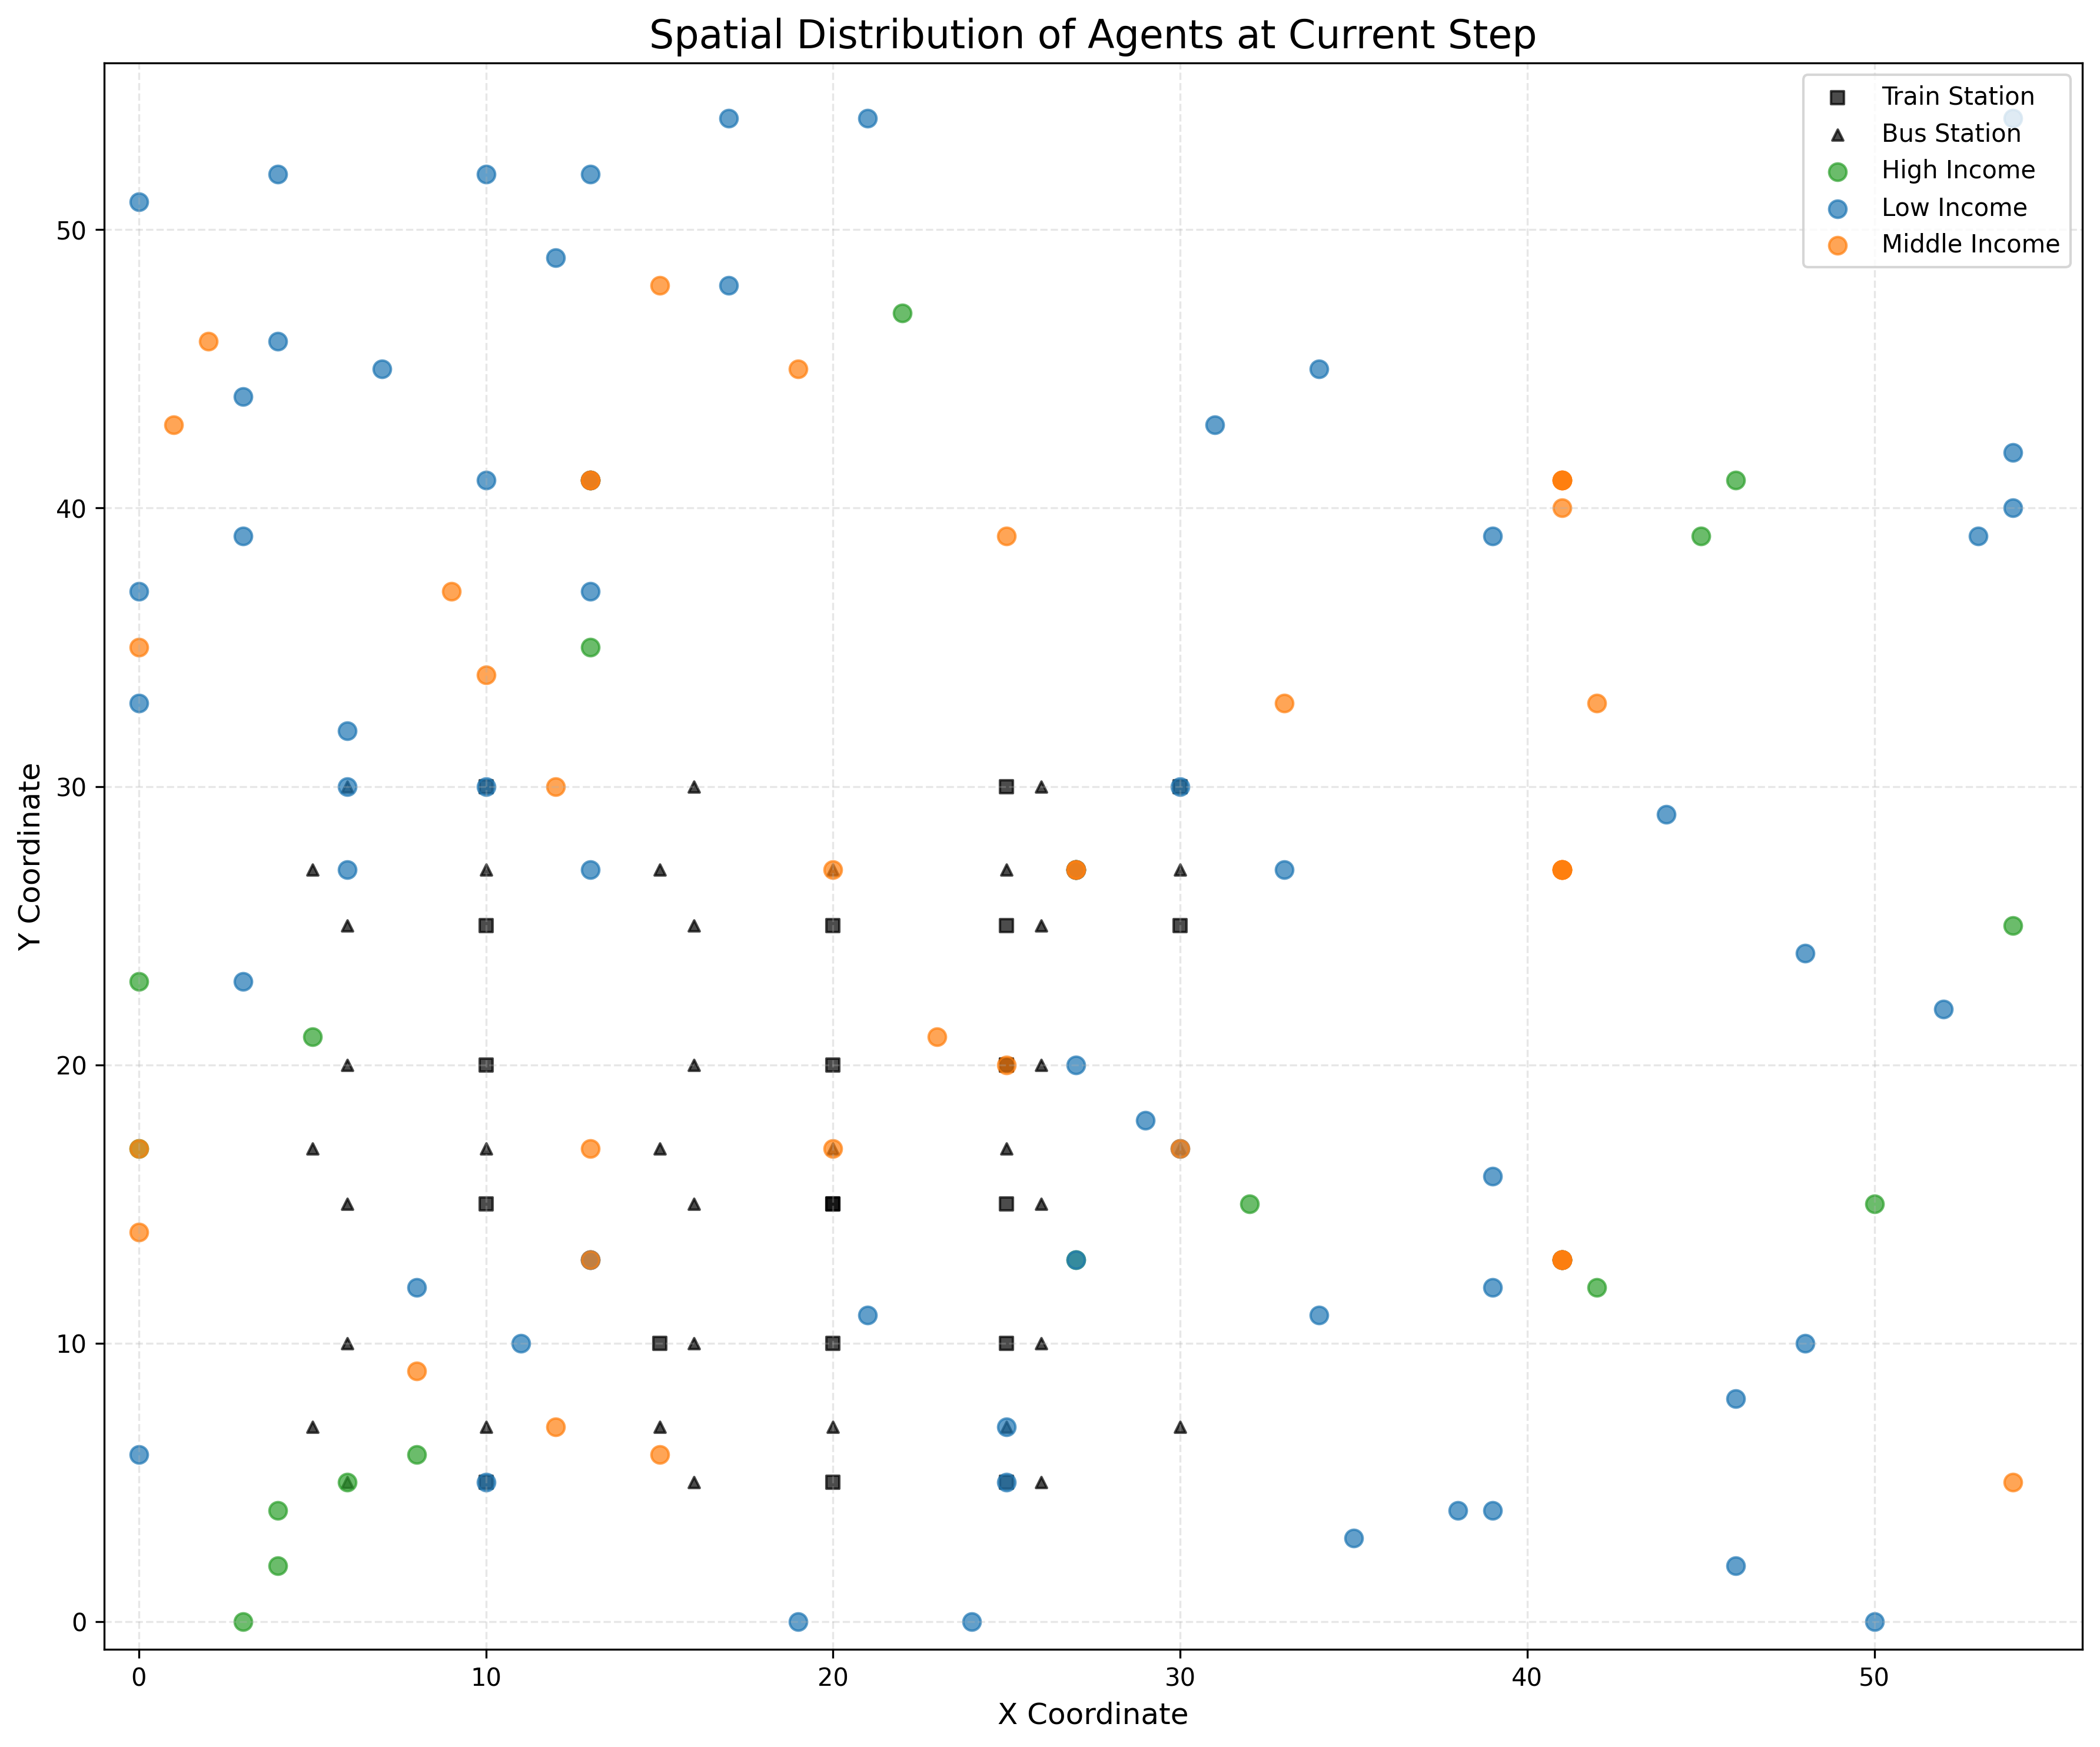
\includegraphics[width=0.8\textwidth]{3_spatial_dist_current_income.png}
\caption{Illustrative spatial distribution of commuter agents by income level in a reduced-resolution visualisation export. The figure is a debugging and presentation view rather than a literal rendering of the 100$\times$100 optimisation environment.}
\label{fig:spatial_distribution}
\end{figure}
Following the mathematical concepts presented in Section \ref{sec:simpleformula}, this section provides a detailed description of the ABM-ETOP simulation process. This comprehensive computational approach operationalises the earlier concepts by integrating heterogeneous agent behaviours, dynamic system interactions, and policy interventions for realistic analysis of transport system dynamics and policy impacts. Figure~\ref{fig:spatial_distribution} illustrates the heterogeneous spatial distribution of commuter agents across different income levels within the simulation environment, demonstrating the framework's capacity to model diverse socioeconomic populations alongside transport infrastructure.

The iterative simulation procedure, formalised in Algorithm 1 (Table~\ref{alg:abm-etop}), begins each time step with \textit{commuter agents} generating trip requests based on their socioeconomic characteristics and activity patterns (line 3). The system coordinator (the \textit{MaaS agent}) then identifies available transport options and calculates route-specific metrics, including travel time and service cost, accounting for congestion effects (line 5). The transport options include public transport (bus and train), shared car services, shared bike services, MaaS bundles, and walking. The \textit{MaaS agent} implements two complementary algorithms for multi-modal routing: a modified Dijkstra algorithm for road-based routing and RAPTOR for public-transport routing. Subsidy policies are applied after the option set is generated, based on the FPS value and PBS allocation matrix for the current simulation, thereby modifying effective traveller costs. Full details of the subsidy mechanism are provided in Appendix~\ref{app:abm_development}. \textit{Commuter agents} then make mode choices through the multinomial logit model (line 11). Behavioural parameters vary by income group, so price and time sensitivities are not identical across travellers. After choices are made, network traffic volumes are updated (line 12) and service providers adjust pricing in response to demand and capacity utilisation (lines 14--16), creating a feedback loop between demand and costs. Figure~\ref{fig:dynamic_pricing} shows an illustrative pricing trace from one simulation output; local price changes need not mirror utilisation spikes one-for-one because each provider updates prices from its own demand-capacity ratio and smoothing rules.

Simultaneously, the \textit{MaaS agent} dynamically updates routing for car-sharing using the BPR function (line 7). As traffic loads accumulate, optimal paths are recalculated to circumvent congestion, producing changing spatiotemporal traffic patterns over the day. These routing adjustments create additional feedback loops between network conditions and travel behaviour. Once a simulation run is complete, the framework calculates the three performance indicators formalised in Algorithm 1 (lines 19--21). The simulation process then feeds those outcomes into the Bayesian optimisation component illustrated in Figure~\ref{fig:simple_flowchart}, which evaluates candidate subsidy allocations using Gaussian-process regression and an Expected Improvement acquisition rule.

The integration of agent-based simulation with Bayesian optimisation supports policy evaluation that captures heterogeneous behaviour, dynamic responses, and system feedback. We emphasise, however, that the present manuscript studies a stylised scenario and should be interpreted as evidence about the framework's behaviour under that scenario, not as a direct real-world deployment claim.
\begin{figure}[!t]
\centering
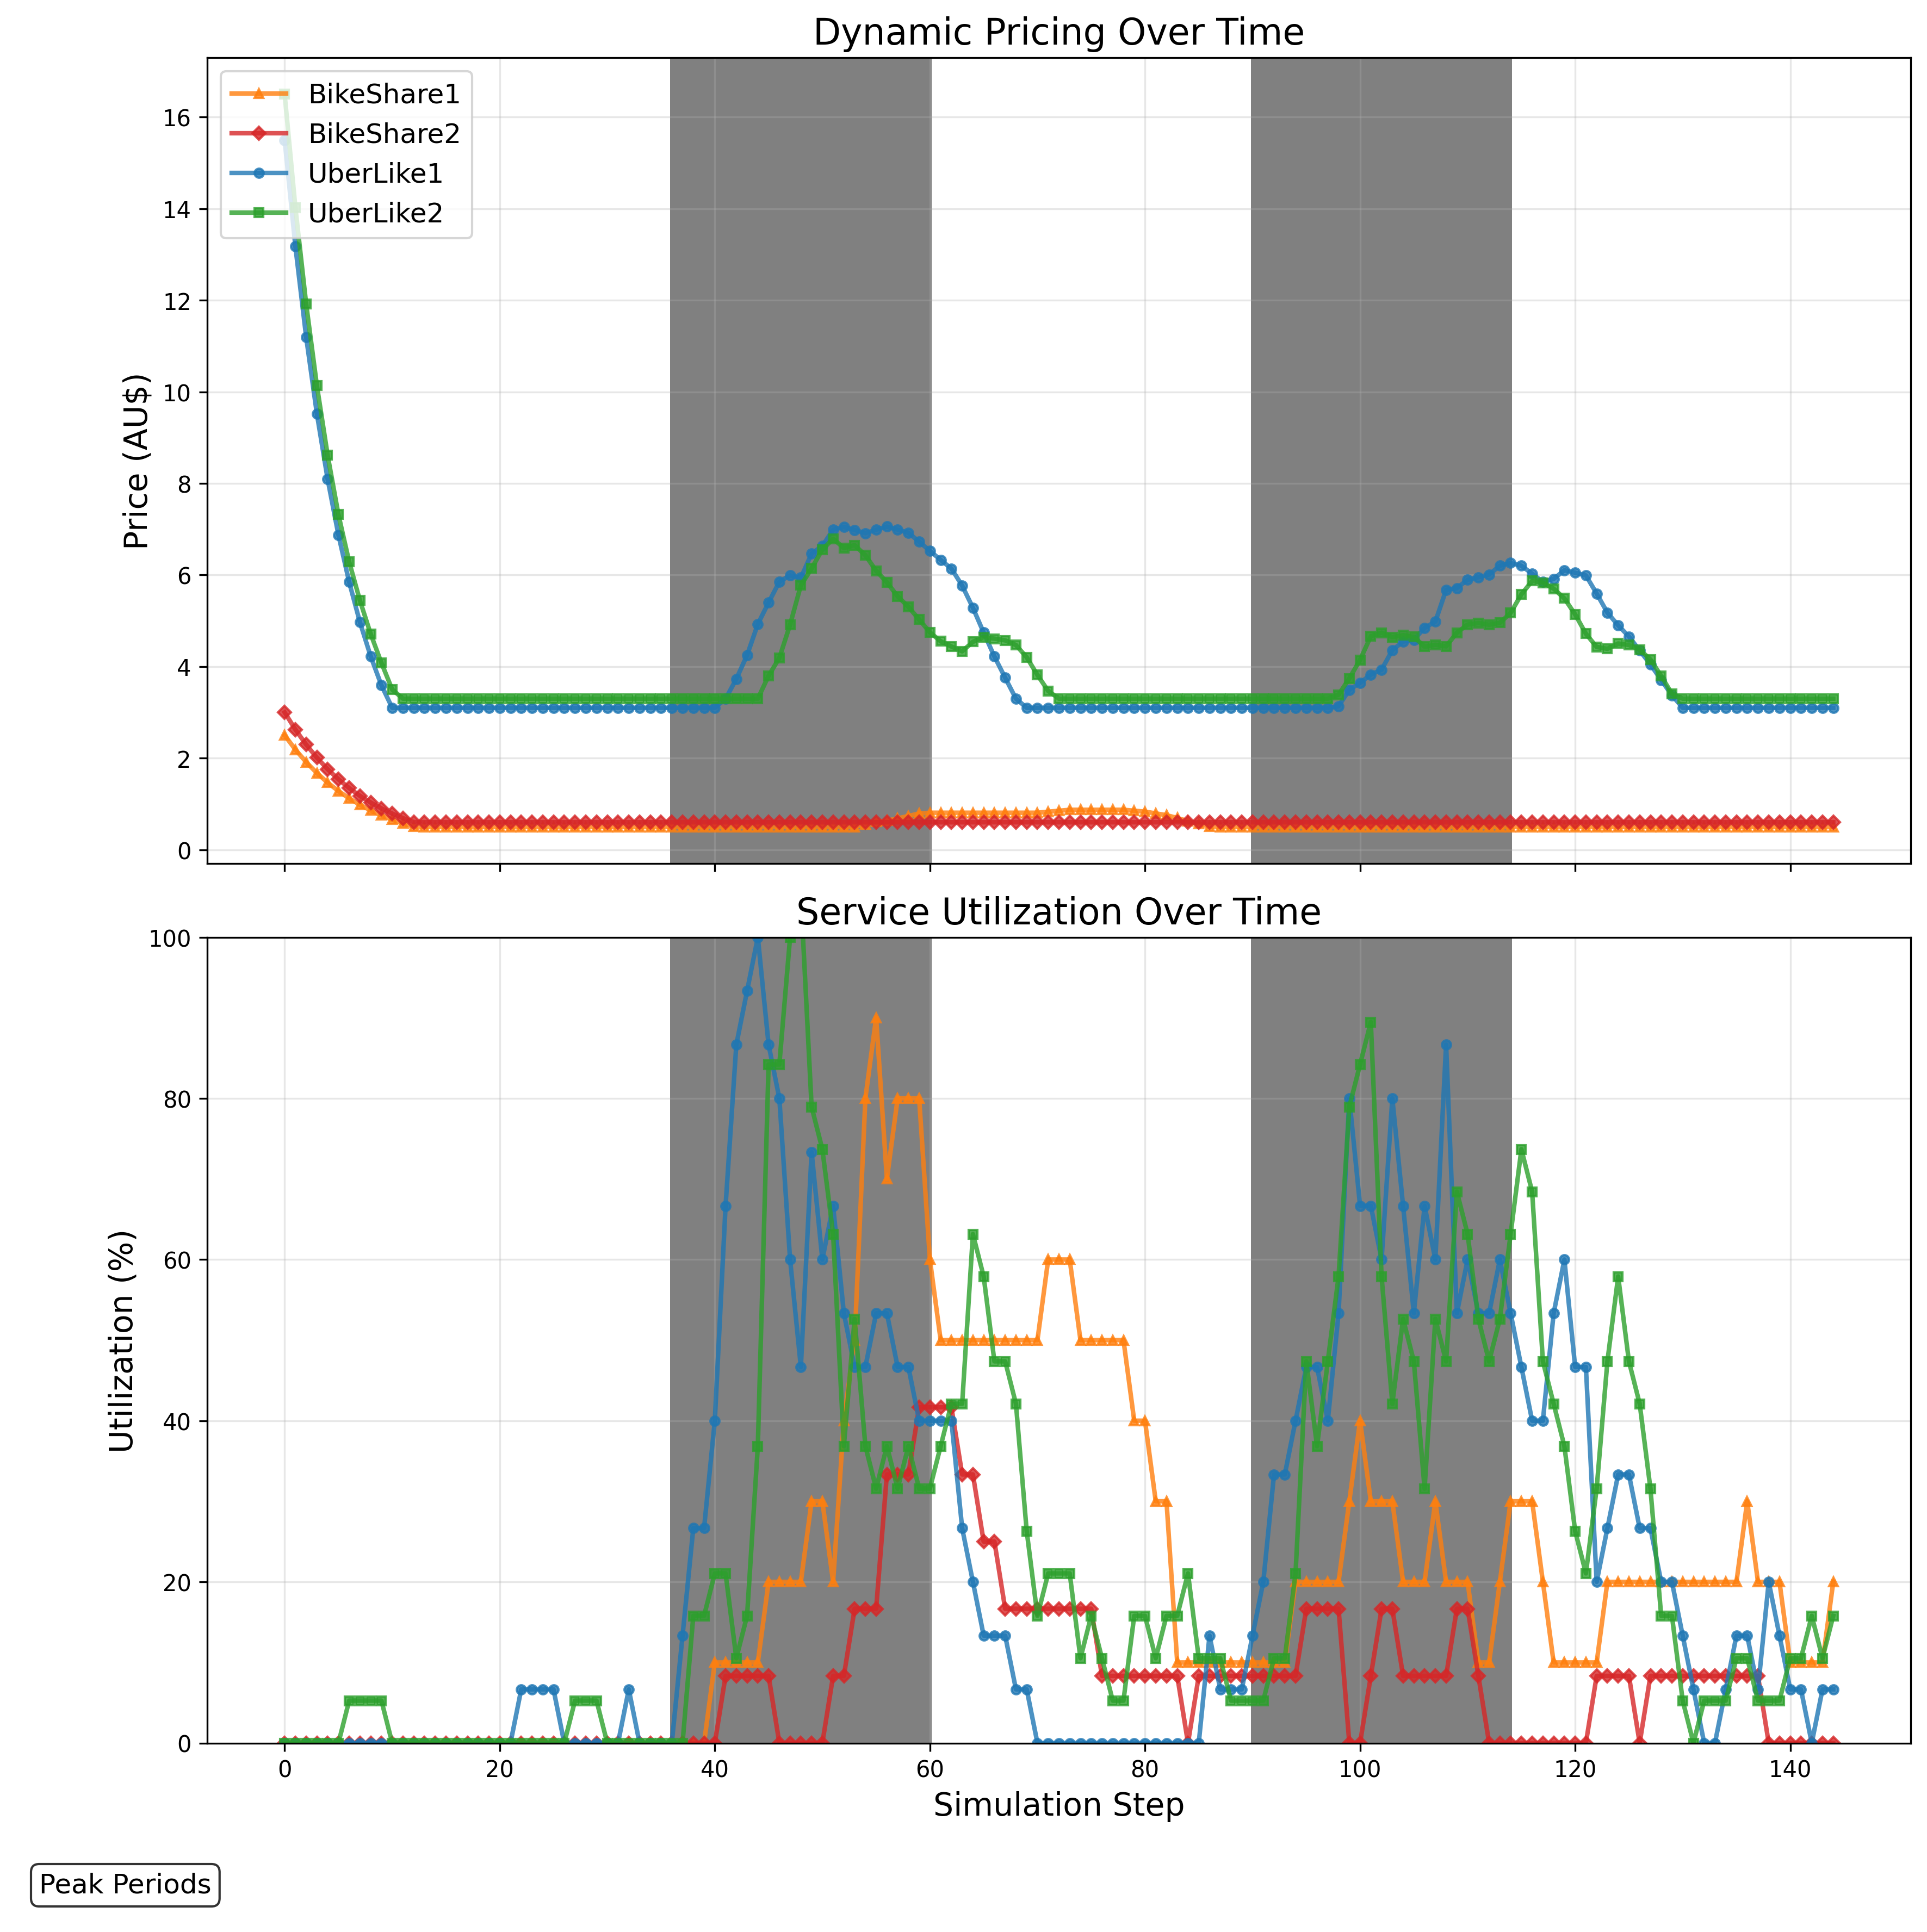
\includegraphics[width=\textwidth]{4_dynamic_pricing_analysis.png}
\caption{Illustrative dynamic pricing and service-utilisation traces from a single simulation output. Provider-specific price movements depend on demand-capacity ratios and smoothing rules, so a local utilisation spike need not produce a proportional instantaneous price spike.}
\label{fig:dynamic_pricing}
\end{figure}
\begin{figure}[!t]
\centering
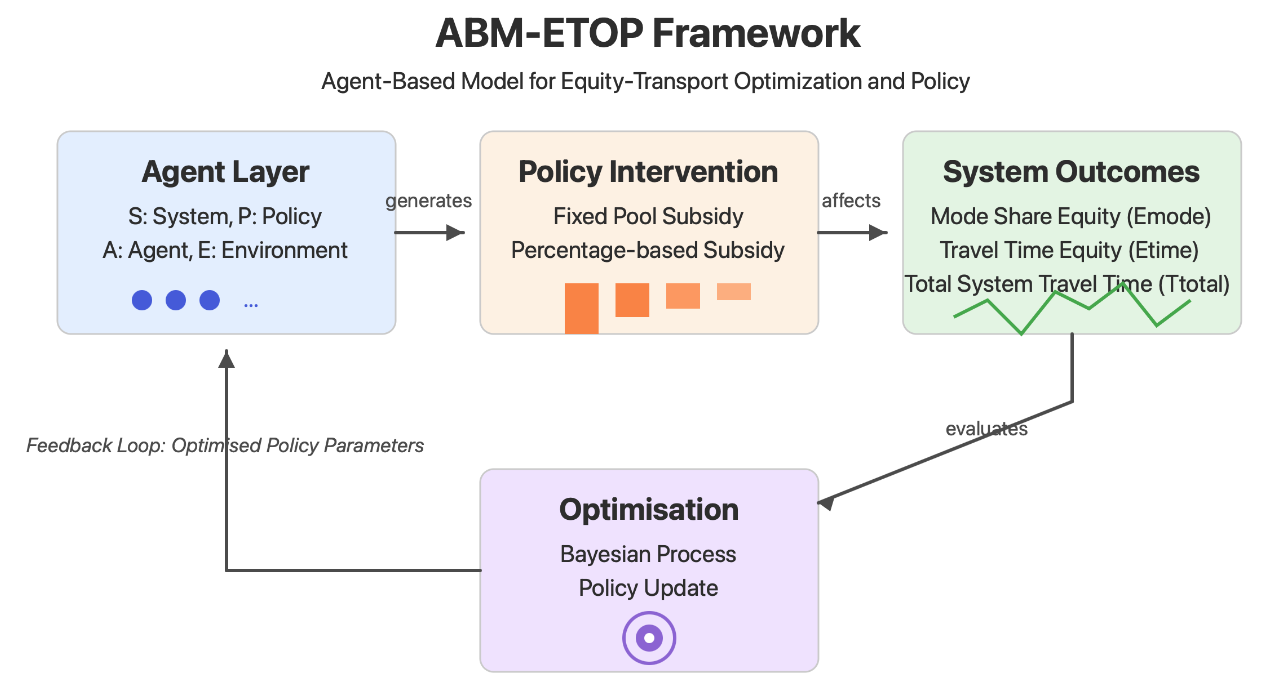
\includegraphics[width=\textwidth]{5_framework_simplified_flowchart.png}
\caption{Process flow of the ABM-ETOP framework showing the continuous feedback loop between simulation and optimisation. The simulation results feed into the Bayesian optimisation process, which iteratively updates policy parameters to identify optimal subsidy allocation strategies.}
\label{fig:simple_flowchart}
\end{figure}

\section{Optimisation Methodology}\label{sec:optimisation}

\subsection{Bayesian Optimisation Implementation}

\begin{table}[width=\textwidth]
\caption{Algorithm 2 Subsidy Allocation Optimisation}
\label{alg:subsidy-opt}
\hrule height 1pt
\vspace{0.5em}
\small
\begin{tabularx}{\textwidth}{p{0.07\textwidth}Y}
& \textbf{Require:} FPS set $\mathcal{F} = \{3500, 4500, 5500, 6500, 7000, 7500, 8000, 8500, 9000, 9500, 10000, 15000\}$; objective-specific configuration; 12 subsidy-allocation variables across 3 income groups and 4 mode classes \\
& \textbf{Ensure:} Objective-specific best $(FPS^*, A^*)$ pairs with repeated-seed summaries \\
1: & \textbf{for} each objective $O \in \{E_{\text{mode}}, E_{\text{time}}, T_{\text{total}}\}$ \textbf{do} \\
2: & \hspace{1em} \textbf{for} each $FPS \in \mathcal{F}$ \textbf{do} \\
3: & \hspace{2em} Draw 8 Latin-hypercube initial allocation matrices with $0.0 \leq a_{i,m} \leq 0.8$ for all income-mode cells \\
4: & \hspace{2em} Run Bayesian optimisation over the 12-dimensional allocation space using a Gaussian-process surrogate and Expected Improvement \\
5: & \hspace{2em} Use 10 BO updates for mode-share equity and 3 BO updates for travel-time equity and total system travel time \\
6: & \hspace{2em} Keep the best allocation found for that $(FPS, O)$ pair \\
7: & \hspace{1em} \textbf{end for} \\
8: & \hspace{1em} Re-evaluate the retained policy for each sampled FPS over 30 stochastic seeds and aggregate mean, standard deviation, and 95\% confidence interval \\
9: & \hspace{1em} Select $FPS_O^*$ by the lowest seed-mean objective value, then summarise budget usage and allocation shares \\
10: & \textbf{end for} \\
11: & Run a deterministic fixed-policy control with fixed commuters, trip requests, and background conditions to interpret stochastic non-monotonicity \\
12: & \textbf{return} the objective-specific optima, repeated-seed summaries, and cross-policy comparison tables \\
\end{tabularx}
\vspace{0.5em}
\hrule height 1pt
\end{table}

The ABM-ETOP framework employs Bayesian optimisation with Gaussian-process regression to identify subsidy-allocation strategies for a fixed FPS budget. The current workflow is mono-objective at the optimisation stage and comparative at the synthesis stage: one optimisation is run for mode-share equity, one for travel-time equity, and one for total system travel time.

\begin{equation}
\mathbf{A}^* = \underset{\mathbf{A}}{\text{argmin}} \, M(\mathbf{A})
\end{equation}

The optimisation process follows the sequential approach outlined in Algorithm 2 (Table \ref{alg:subsidy-opt}). The 12 dimensions arise from 3 income groups crossed with 4 mode classes. The audited scripts apply the same bounds, $0.0 \leq a_{i,m} \leq 0.8$, to every decision variable; the revised manuscript therefore does not treat progressive allocation as a hard-coded consequence of unequal bounds. Each FPS value begins from 8 Latin-hypercube initial allocations. The mode-share objective then receives 10 Bayesian-optimisation updates per FPS value, while the travel-time equity and total-system-travel-time objectives each receive 3 updates per FPS value. The simulation horizon of 144 time steps represents within-run time resolution and should not be confused with the number of optimisation iterations.

Addressing the high computational cost of ABM evaluation, Bayesian optimisation offers a practical alternative to exhaustive grid search. The surrogate model screens the search space and concentrates simulation effort on promising allocations while still permitting exploration of uncertain regions. The same optimisation logic is then followed by a repeated-seed evaluation stage. For each sampled FPS value, the retained policy is re-run over 30 stochastic seeds and aggregated into mean, standard deviation, and 95\% confidence interval summaries. Those merged summaries, rather than the earlier single-run outputs, are the primary quantitative evidence used in this revision.

\subsection{Equilibrium Mechanisms and System Dynamics}
The agent-based architecture represents system feedback that is difficult to express in closed-form equation systems. Peak-period congestion, changing generalised costs, and variable subsidy uptake arise from the interaction of commuter decisions, provider behaviour, and network conditions during the simulation. This joint representation of utility, market, and network processes is also why the stochastic FPS curves can look irregular when trip generation and congestion evolve endogenously.

To interpret that irregularity, the revised workflow adds a deterministic fixed-policy control experiment in which commuters, trip requests, and background conditions are held fixed across FPS values. In the deterministic control, the measured equity response becomes monotonic or near-monotonic until subsidy saturation. We interpret this as supporting evidence that the non-monotonic behaviour in the stochastic summaries stems from ABM randomness and evolving system states rather than from broken optimisation logic. This is a mechanism check, not proof that every stochastic fluctuation is negligible.

\subsection{Robustness, Deterministic Control, and Reproducibility}
The optimisation and re-evaluation scripts reported in this revision are:
\begin{itemize}[leftmargin=*, nosep]
    \item \texttt{mode\_share\_optimization.py}
    \item \texttt{travel\_time\_equity\_optimization.py}
    \item \texttt{total\_system\_travel\_time\_optimization.py}
    \item \texttt{evaluate\_mode\_share\_seeds.py}
\end{itemize}

Their outputs are aggregated through the merged summary folders used throughout this manuscript. Deterministic control experiments are documented in \texttt{README\_DETERMINISTIC.md} and the fixed-policy FPS sweep outputs.

The codebase used for the revised evidence package is available at \url{https://github.com/Rebeccca2000/ABM_ETOP_framework}. Reproducibility in the present study means that readers can inspect the optimisation scripts, the merged seed summaries, the deterministic-control workflow, and the regenerated cross-policy comparison outputs used in the manuscript. Full city-scale calibration remains future work.

\section{Policy Analysis Results}\label{sec:results}
We evaluate how transport subsidies affect inequitable access to mobility options across income groups using the three metrics defined in Section \ref{sec:metricequations}. The revised optimisation scripts use a 100$\times$100 grid, 200 commuters with income weights $[0.5, 0.3, 0.2]$, background traffic of 200 units, and a one-day simulation horizon of 144 time steps. The sampled FPS values are 3,500, 4,500, 5,500, 6,500, 7,000, 7,500, 8,000, 8,500, 9,000, 9,500, 10,000, and 15,000 model units.

All results reported below come from merged seed summaries with $n=30$ per sampled FPS value. The FPS values remain abstract model units and are not converted here into real-world currency. We therefore avoid the earlier baseline-percentage framing and interpret the sampled FPS set directly.

\subsection{Mode Share Equity Analysis}

\subsubsection{Optimal Subsidy Allocation Results}
\begin{figure}[!t]
\centering
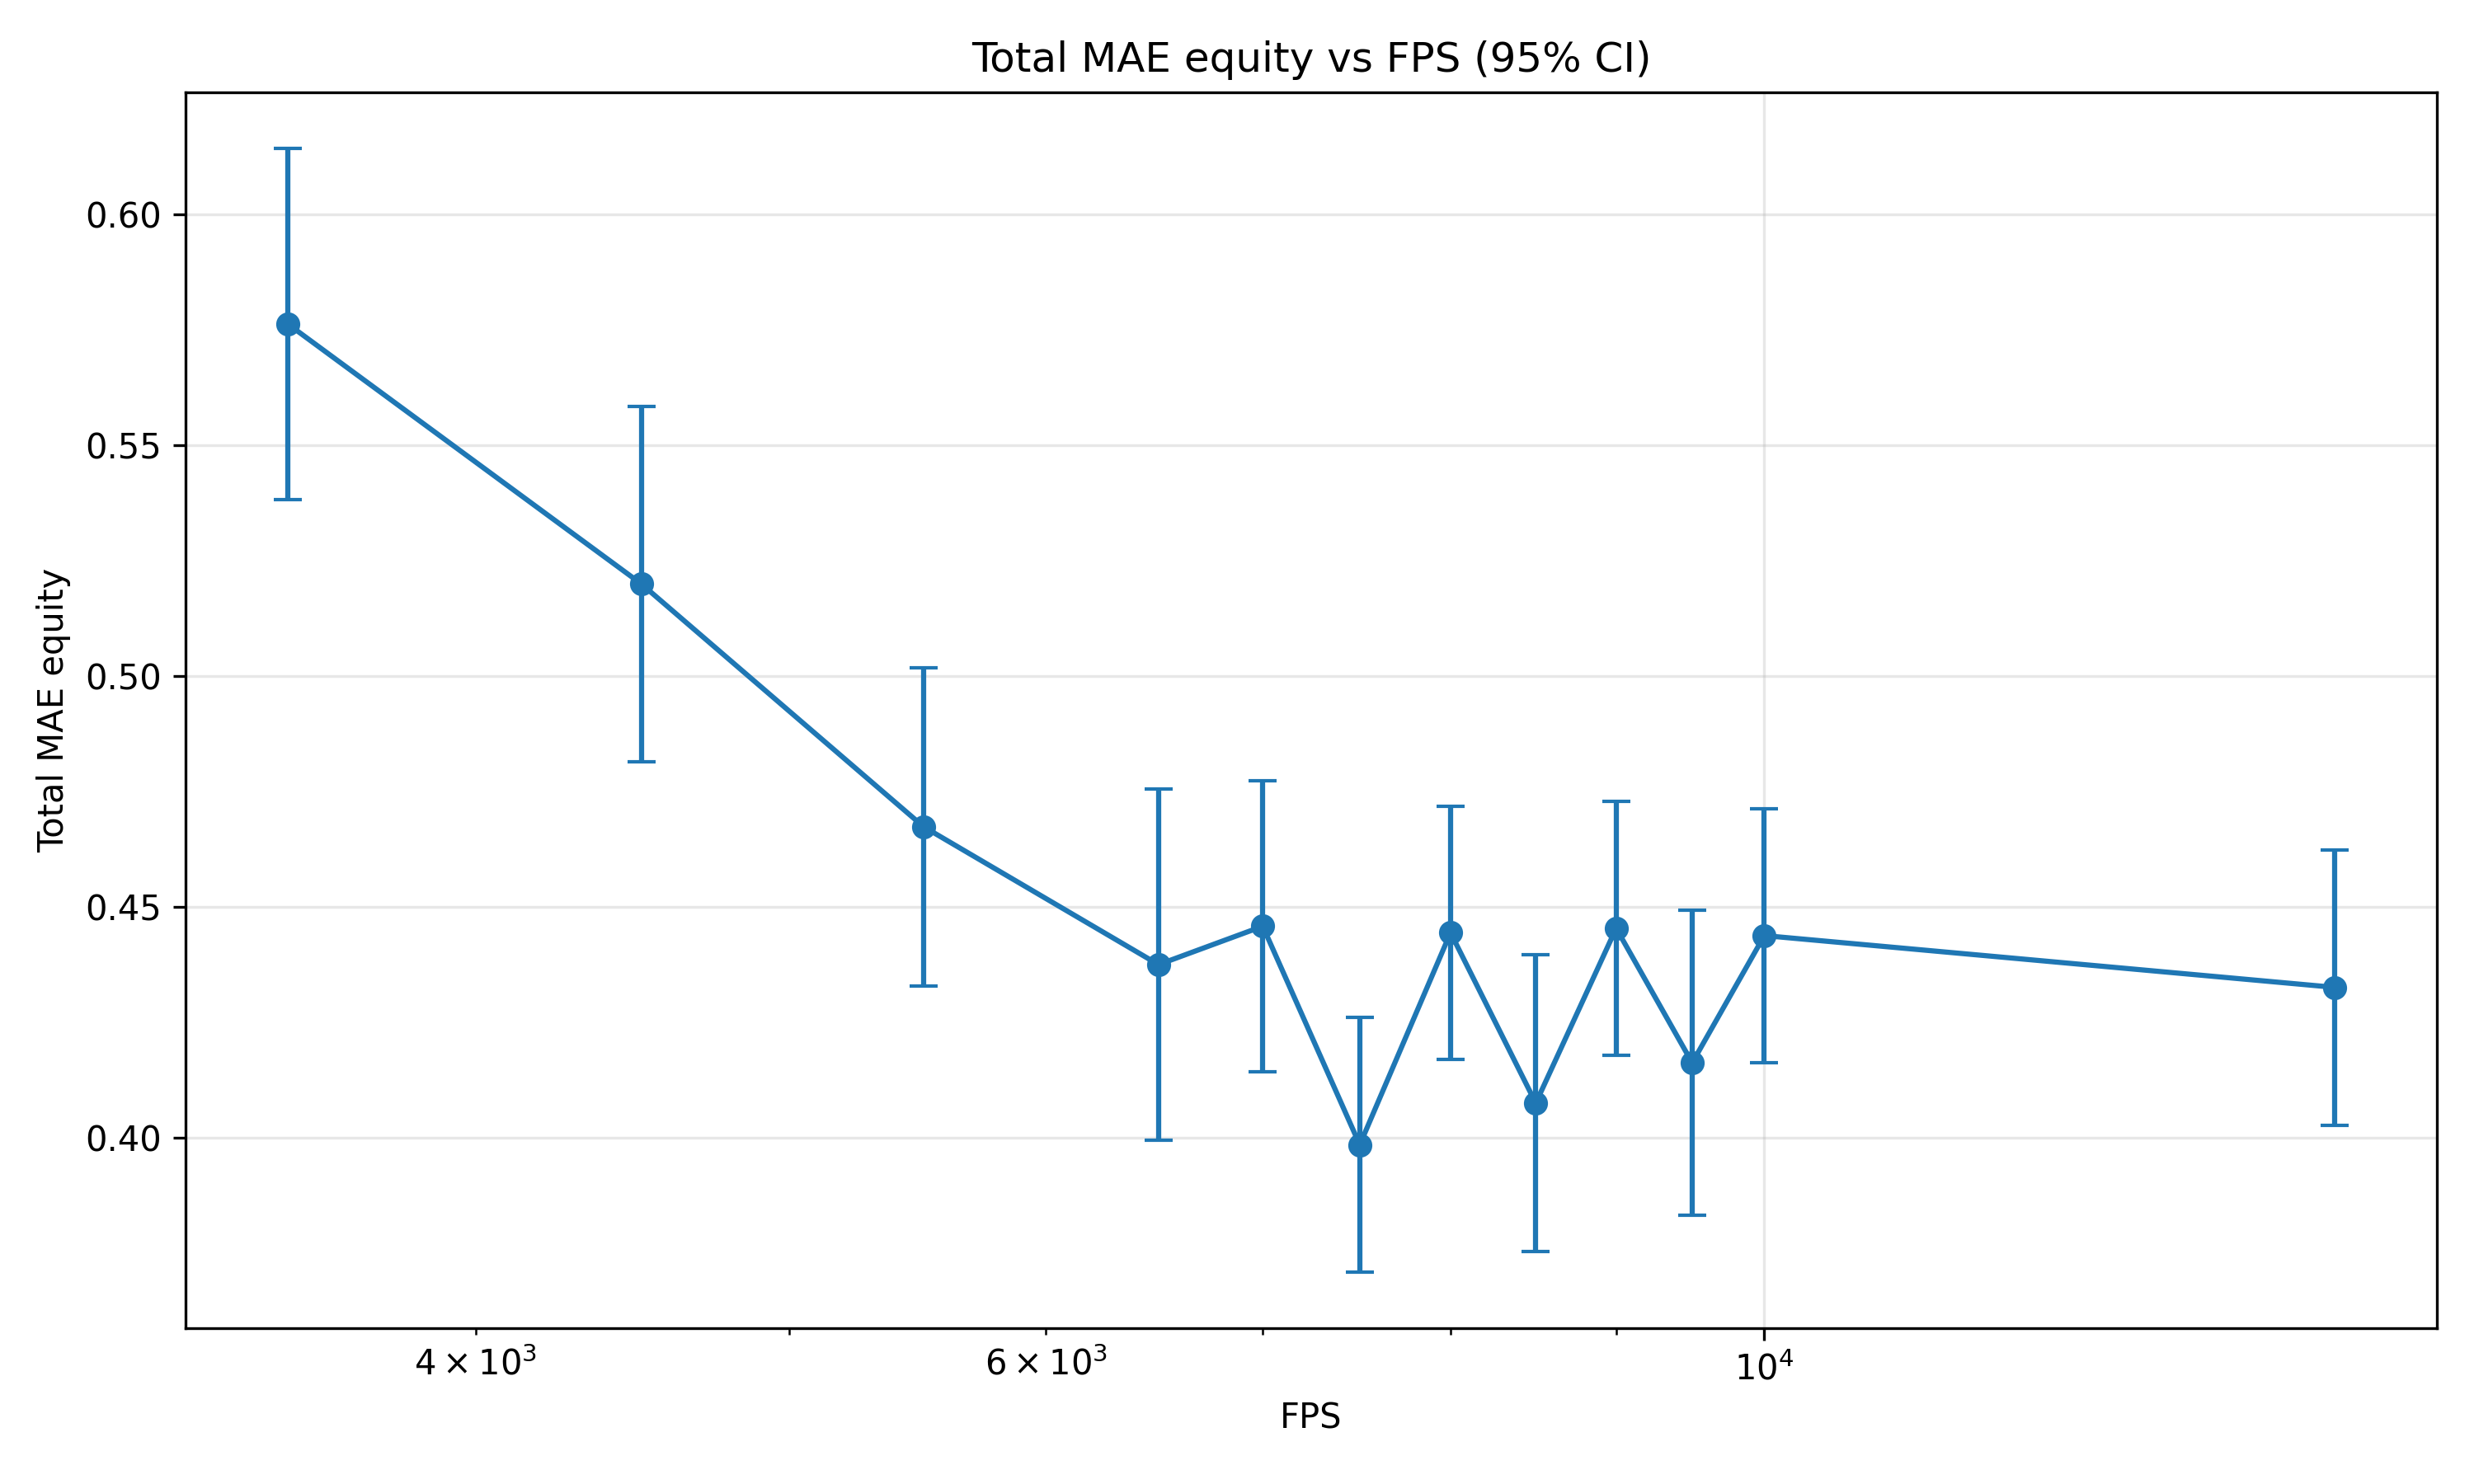
\includegraphics[width=1\textwidth]{mode_share_equity_ci95.png}
\caption{Mode-share equity by FPS from the 30-seed merged evaluation. Points show the mean objective value and error bars show the 95\% confidence interval. The lowest mean occurs at FPS 7,500.}
\label{fig:mode_share_equity_scores}
\end{figure}

\noindent The lowest mean mode-share equity occurs at FPS 7,500 with $E_{\text{mode}} = 0.3984 \pm 0.0276$ (95\% CI, $n=30$). The surrounding values at FPS 8,500 and 9,500 remain competitive, which is why the regenerated cross-policy recommendations treat FPS 7,500--9,500 as the relevant operating range rather than a single exact threshold. Budget usage at the best mean point is $81.46\% \pm 6.48$ percentage points. Figure~\ref{fig:mode_share_equity_scores} shows that the stochastic curve is irregular rather than smoothly monotonic, so the revised interpretation emphasises uncertainty bands instead of a single deterministic turning point.

At the 7,500 optimum, the mean aggregate allocation shares by income group are 38.74\% for low income, 34.91\% for middle income, and 26.35\% for high income. The largest mean allocation components are low-income car (0.7723), low-income bike (0.5963), and middle-income car (0.5875). The revised evidence therefore still favours stronger support for disadvantaged travellers, but not through the earlier 55--65\% low-income allocation claim. Because all twelve allocation variables were optimised over the same 0.0--0.8 bounds, we describe this distribution as an empirical outcome of the revised experiments rather than a pattern imposed by the bound structure. These shares are also not mechanically equal to population shares: they are aggregated from the optimised allocation matrix and realised subsidy uptake, although the larger low-income population share still contributes to observed usage totals.

\subsubsection{Implementation Efficiency and Distribution}
\begin{figure}[!t]
\centering
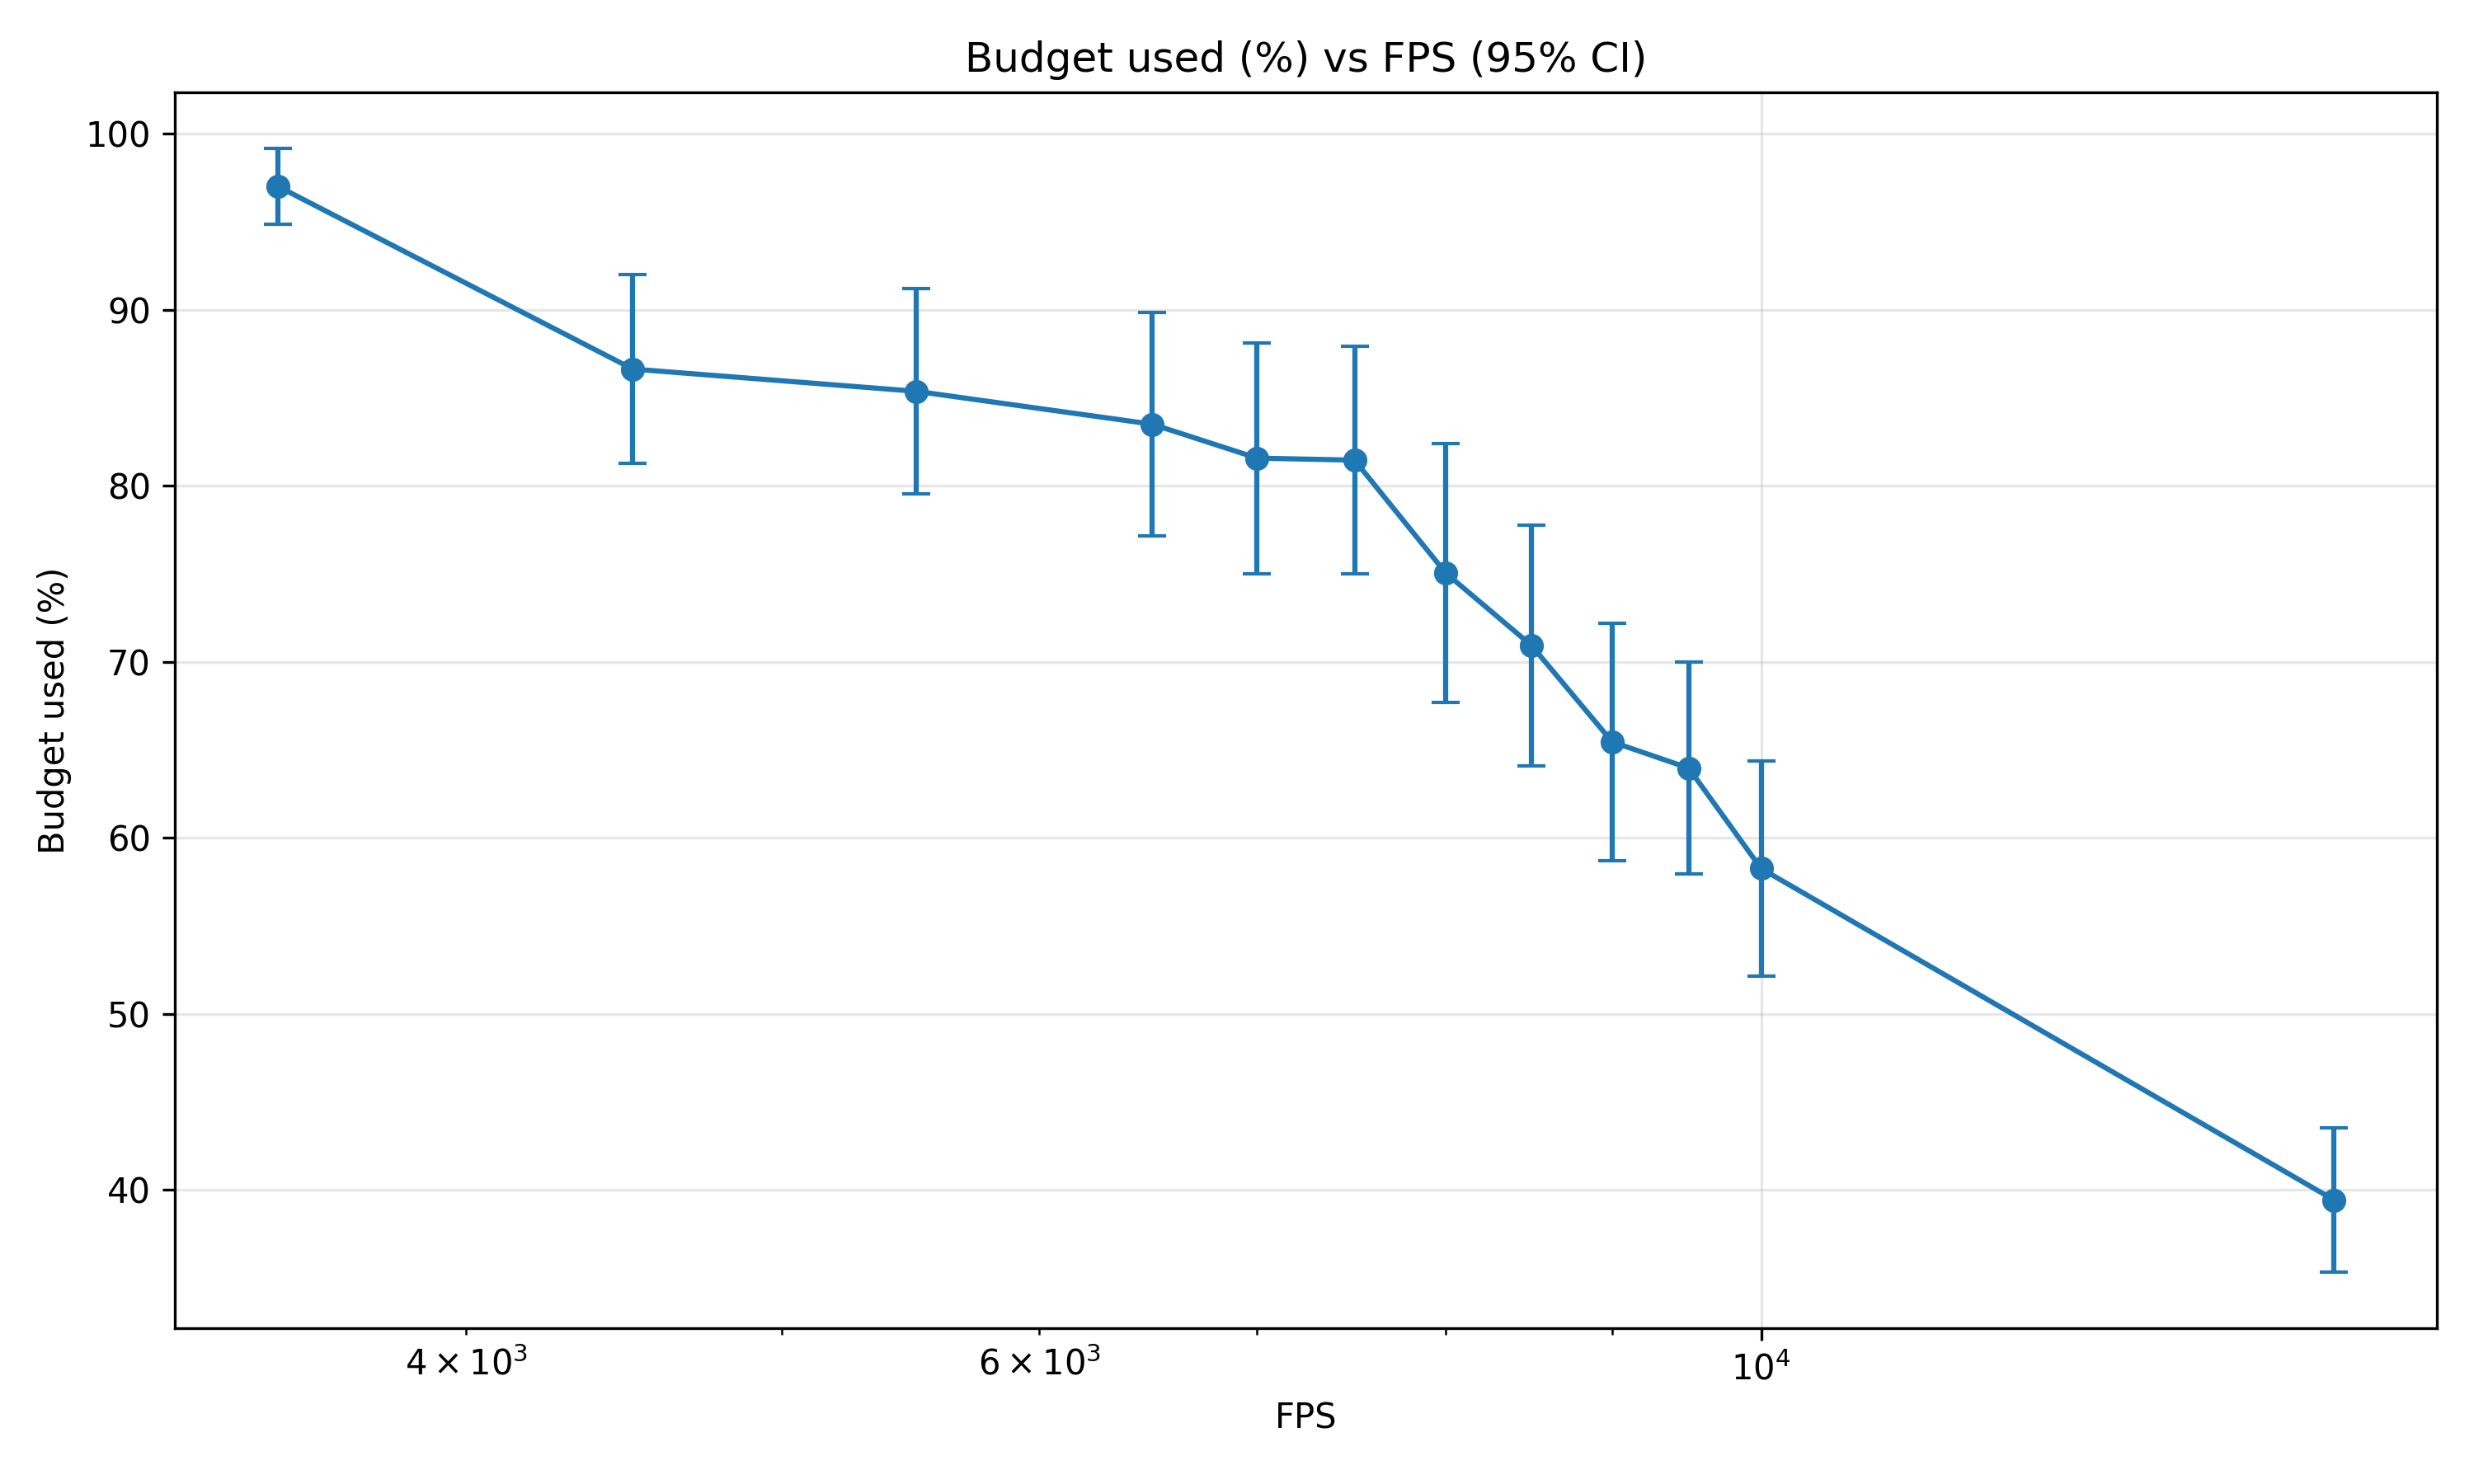
\includegraphics[width=1\textwidth]{mode_share_budget_used_ci95.png}
\caption{Budget used percentage for the mode-share-equity objective across sampled FPS values. Means and 95\% confidence intervals come from the 30-seed merged evaluation.}
\label{fig:subsidy_usage_mode_share}
\end{figure}

\begin{figure}[!t]
\centering
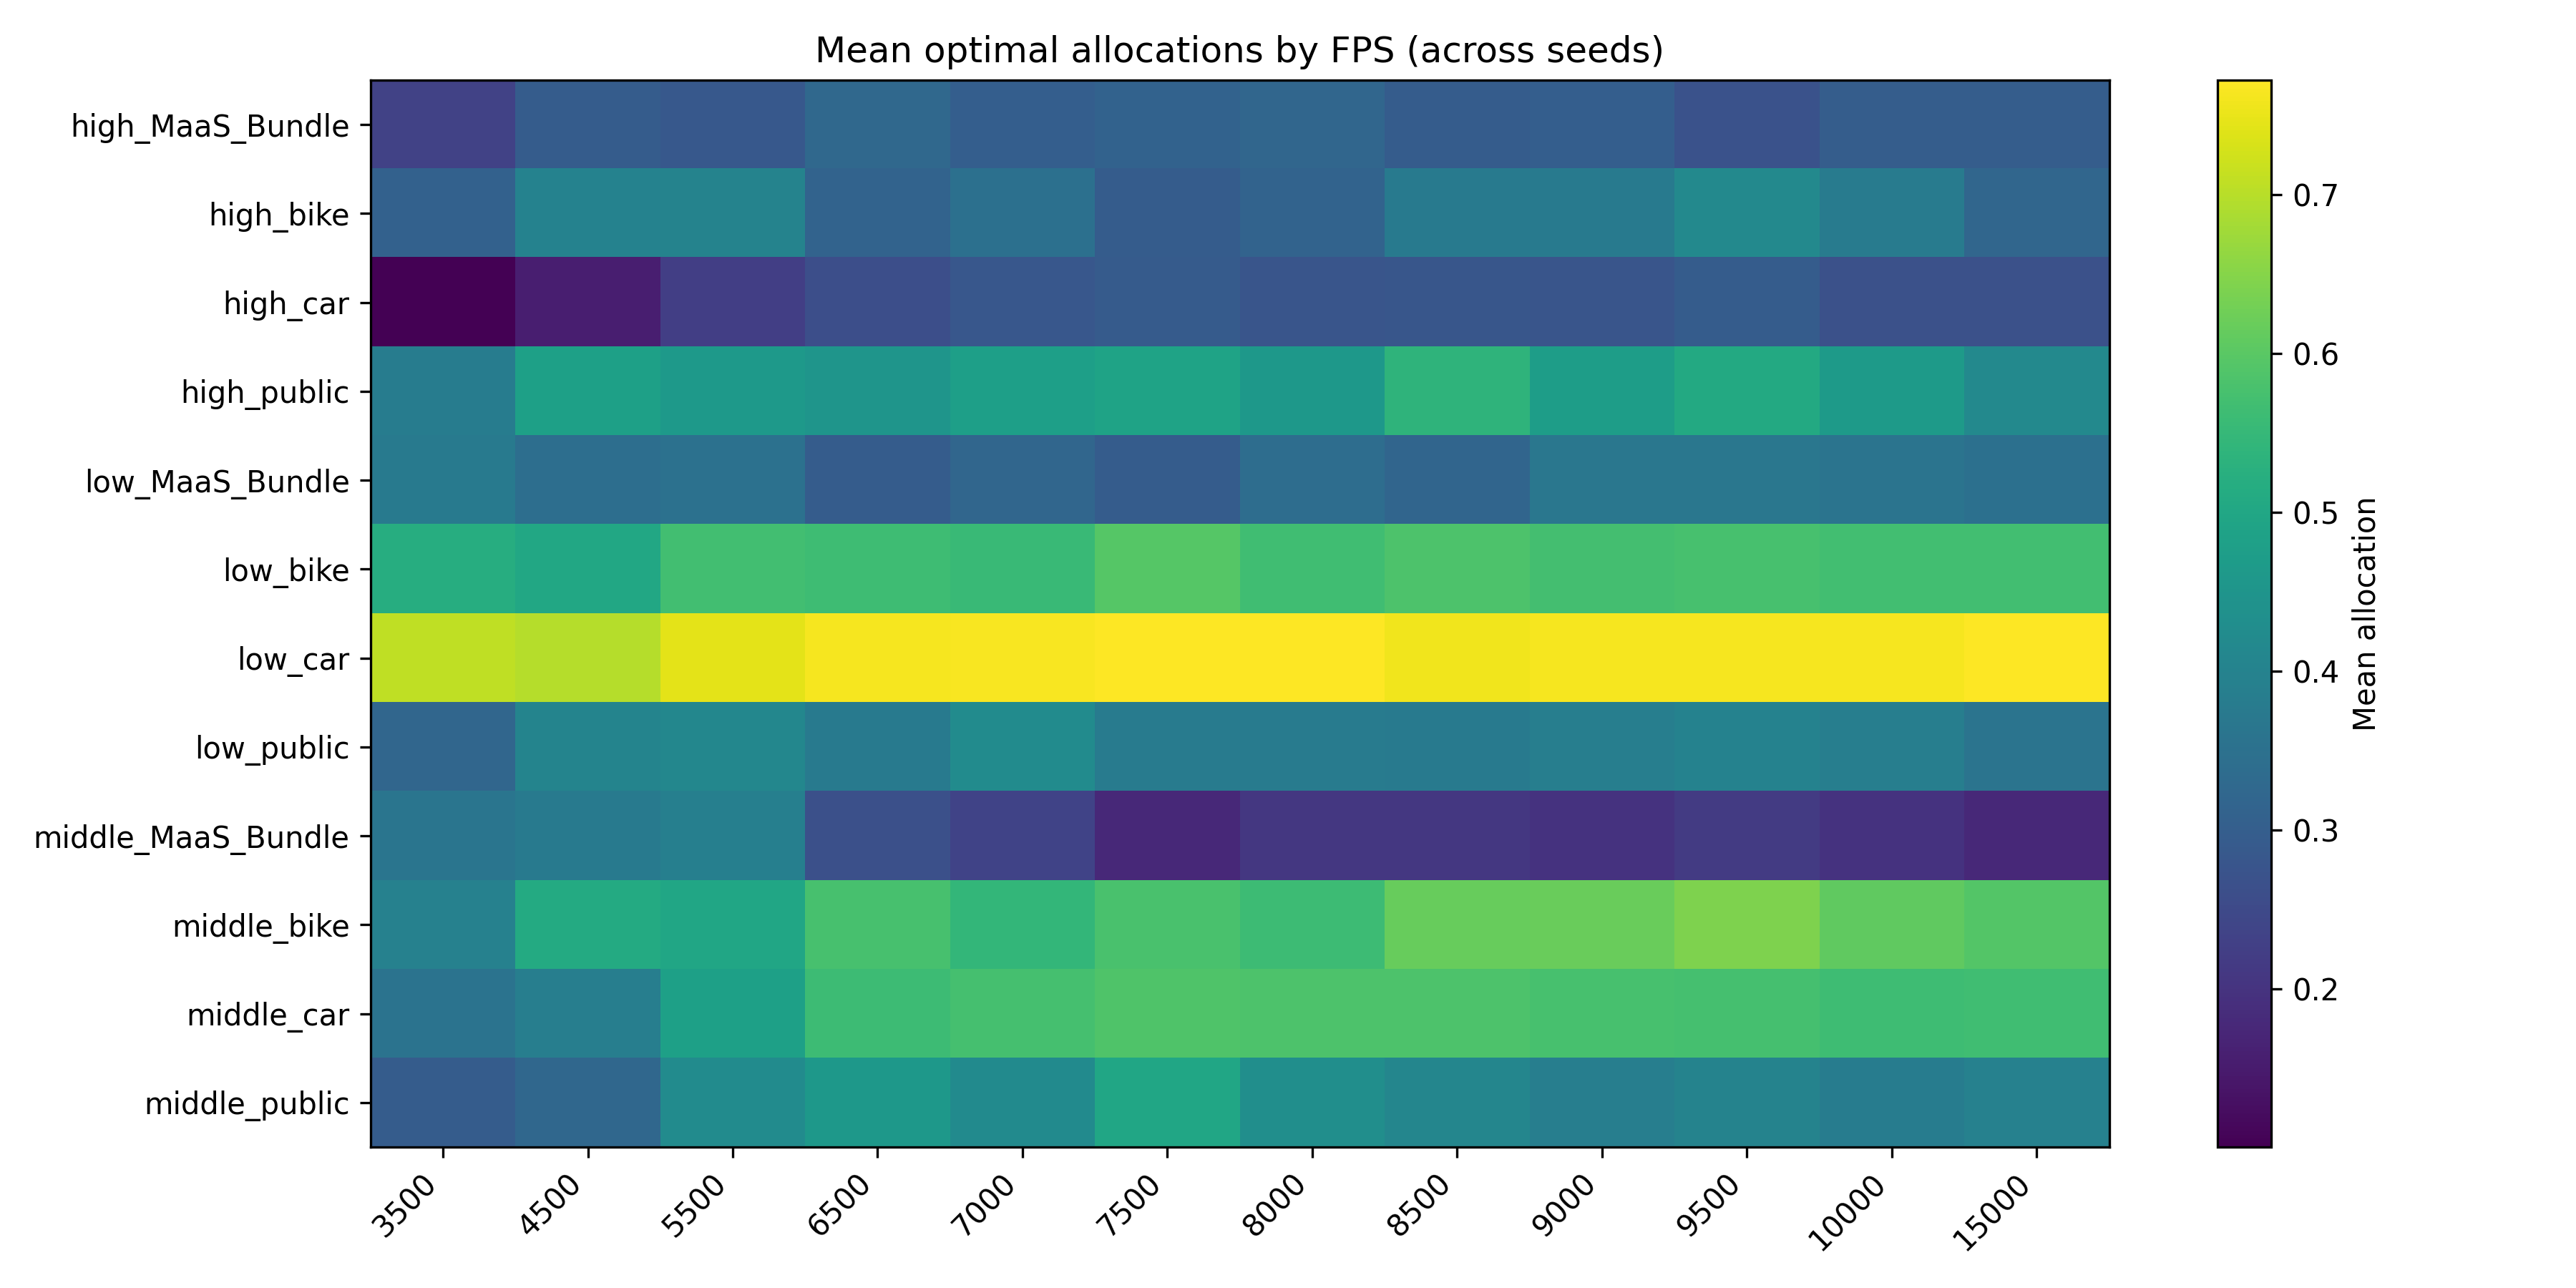
\includegraphics[width=0.9\textwidth]{mode_share_allocation_heatmap.png}
\caption{Mean subsidy-allocation heatmap for the mode-share-equity seed summary. The colour scale shows the mean allocation percentage by income group and mode at each sampled FPS value.}
\label{fig:subsidy_distribution_by_income_mode_share}
\end{figure}

Budget usage declines as FPS increases, even when the objective remains competitive. This matters because the best mean mode-share value occurs at an FPS where the system still deploys most, but not all, of the available subsidy budget. That is consistent with a saturation story: beyond a point, additional budget authority does not translate into proportionate realised subsidy use.

\subsection{Travel Time Equity Analysis}

\subsubsection{Optimisation Approach and Results}
\begin{figure}[!t]
\centering
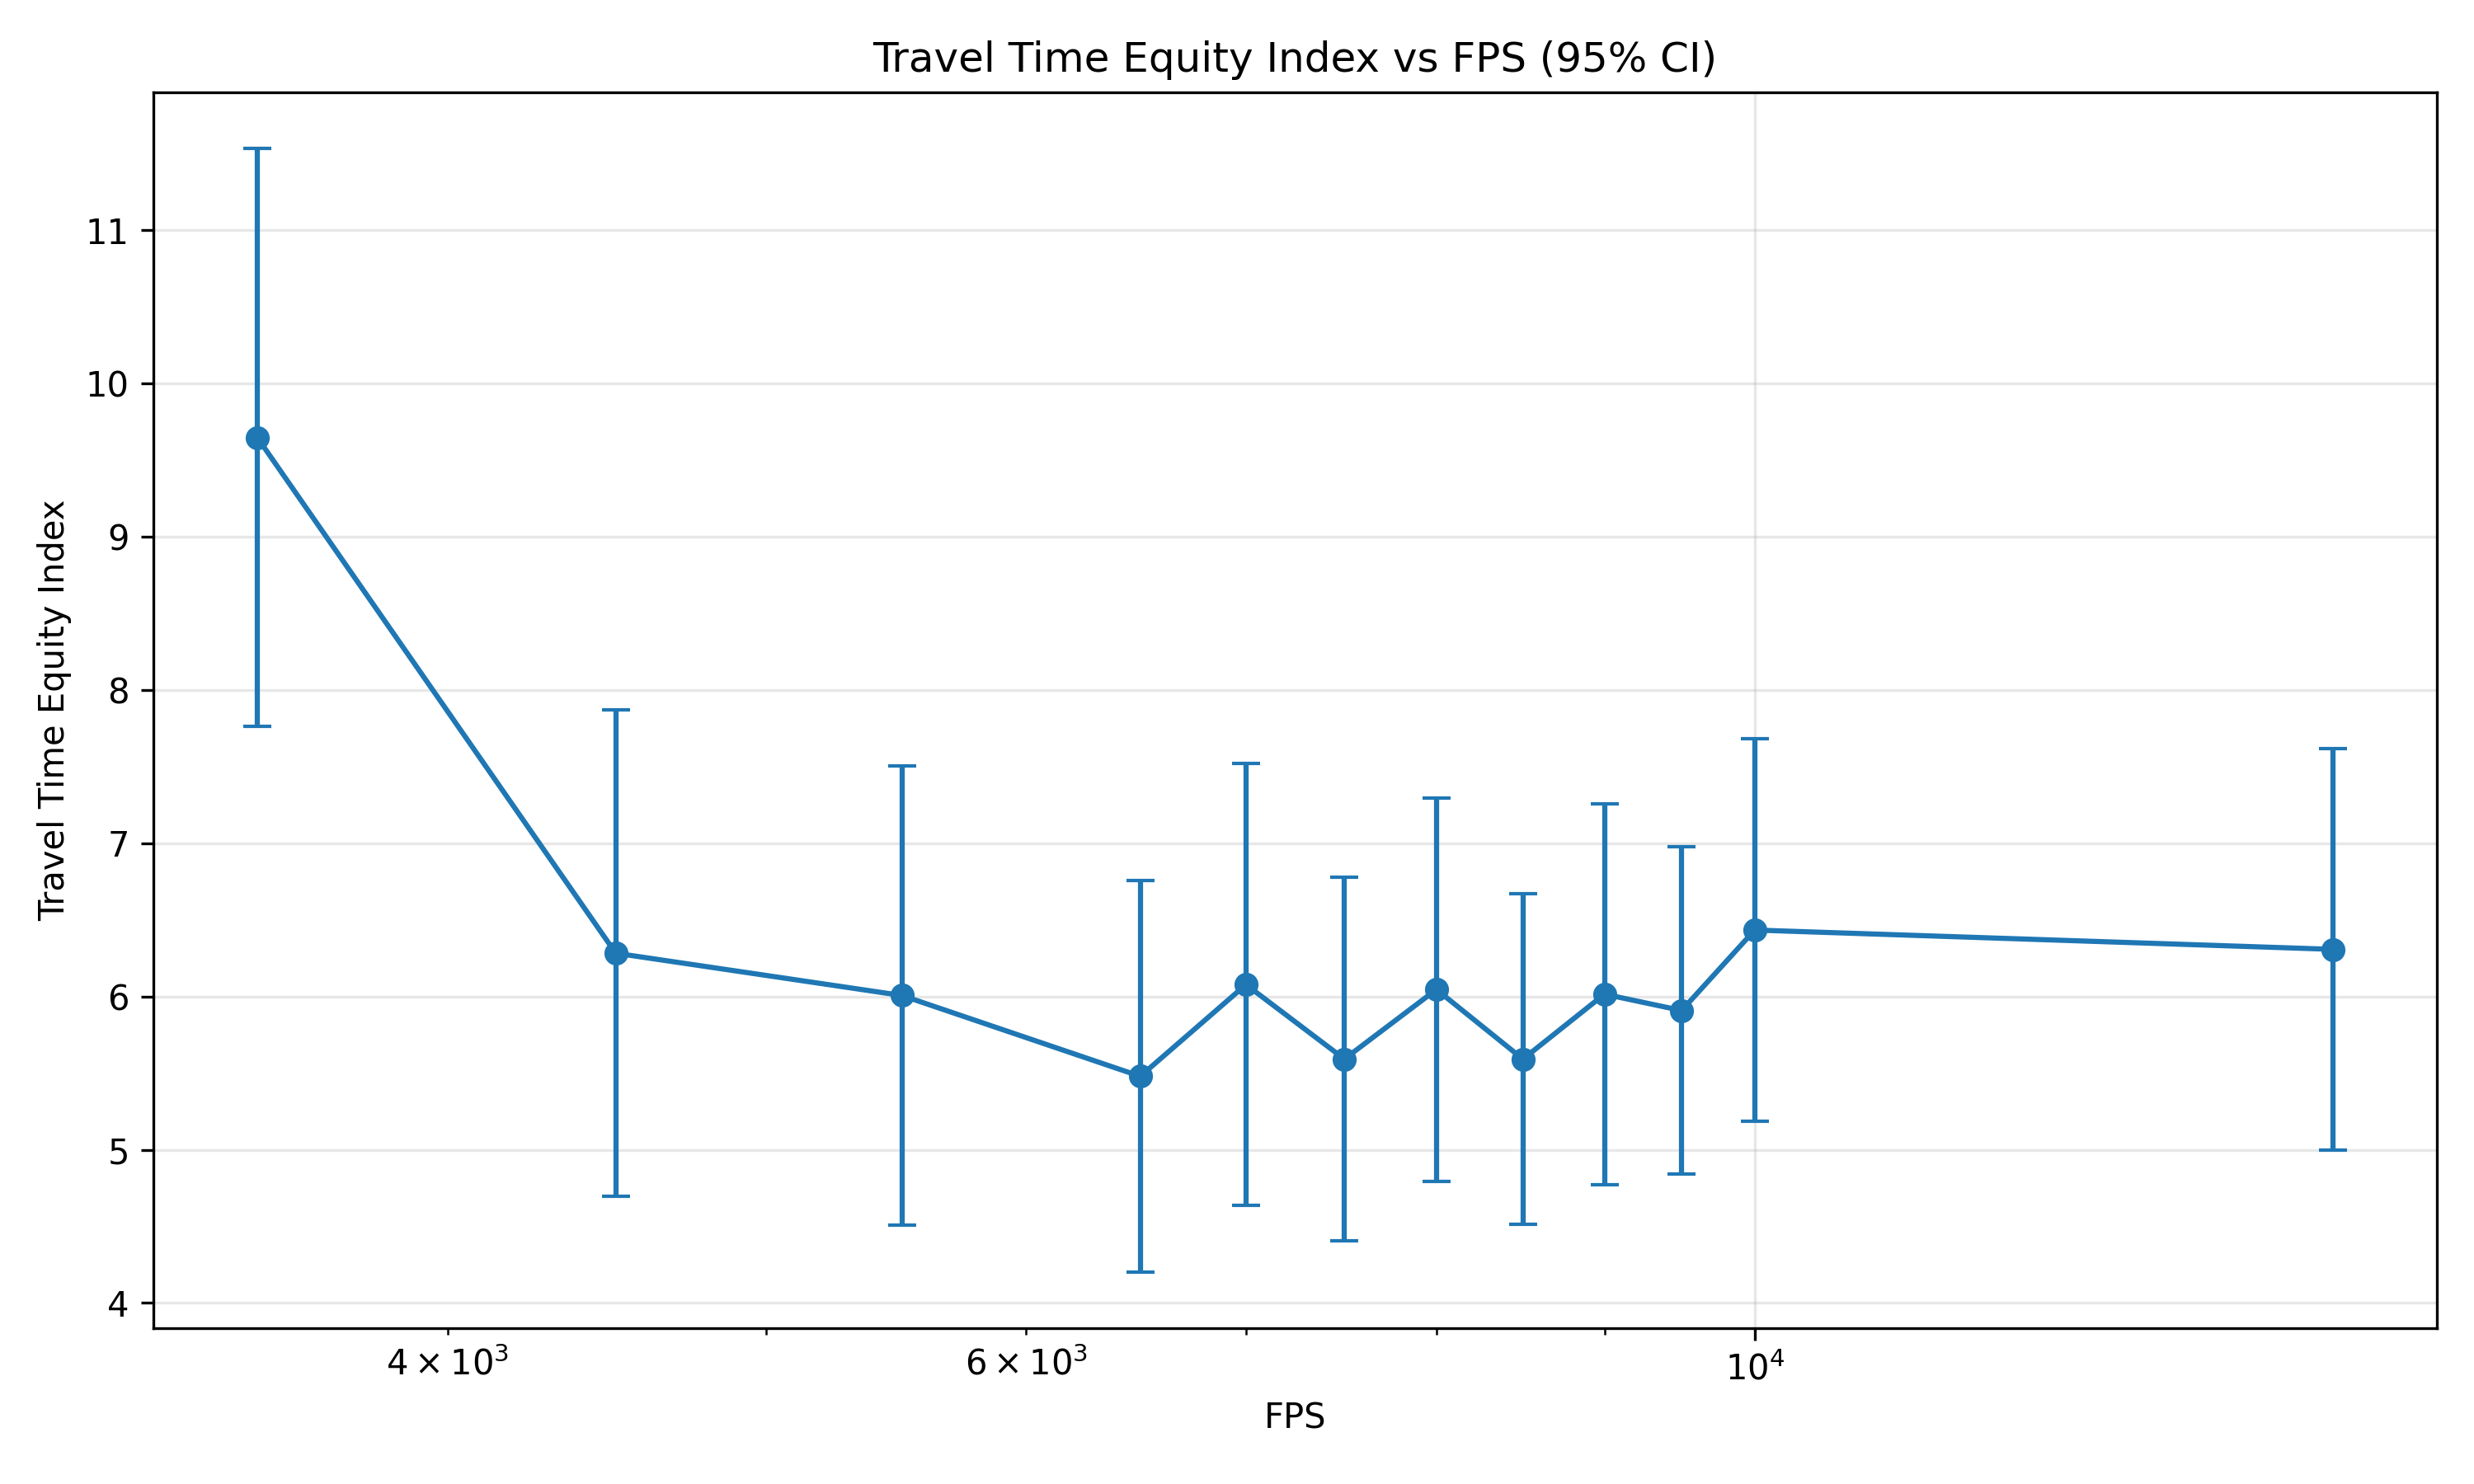
\includegraphics[width=1\textwidth]{travel_time_equity_ci95.png}
\caption{Travel-time equity by FPS from the 30-seed merged evaluation. Means and 95\% confidence intervals are shown for each sampled FPS value. The lowest mean occurs at FPS 6,500.}
\label{fig:travel_time_equity_FPS}
\end{figure}

\noindent The best mean travel-time equity occurs at FPS 6,500 with $E_{\text{time}} = 5.4794 \pm 1.2789$ minutes (95\% CI, $n=30$), followed closely by FPS 7,500 and 8,500 on overlapping uncertainty bands. This is why the regenerated policy recommendation treats FPS 6,500--8,500 as the relevant travel-time-equity operating range. Budget usage at the best mean point is $76.32\% \pm 6.29$ percentage points.

The allocation pattern at the 6,500 optimum again places the largest aggregate share with low-income travellers: 41.57\% for low income, 29.78\% for middle income, and 28.65\% for high income. The three highest mean allocation components are low-income car (0.7459), low-income bike (0.5347), and high-income bike (0.5147). The presence of a high-income bike term among the leading allocations is important because it shows that the optimiser is not simply pushing all support toward one group or one mode. Instead, it balances temporal burdens across the system through a mixed allocation profile.

\subsubsection{Implementation Efficiency}
\begin{figure}[!t]
\centering
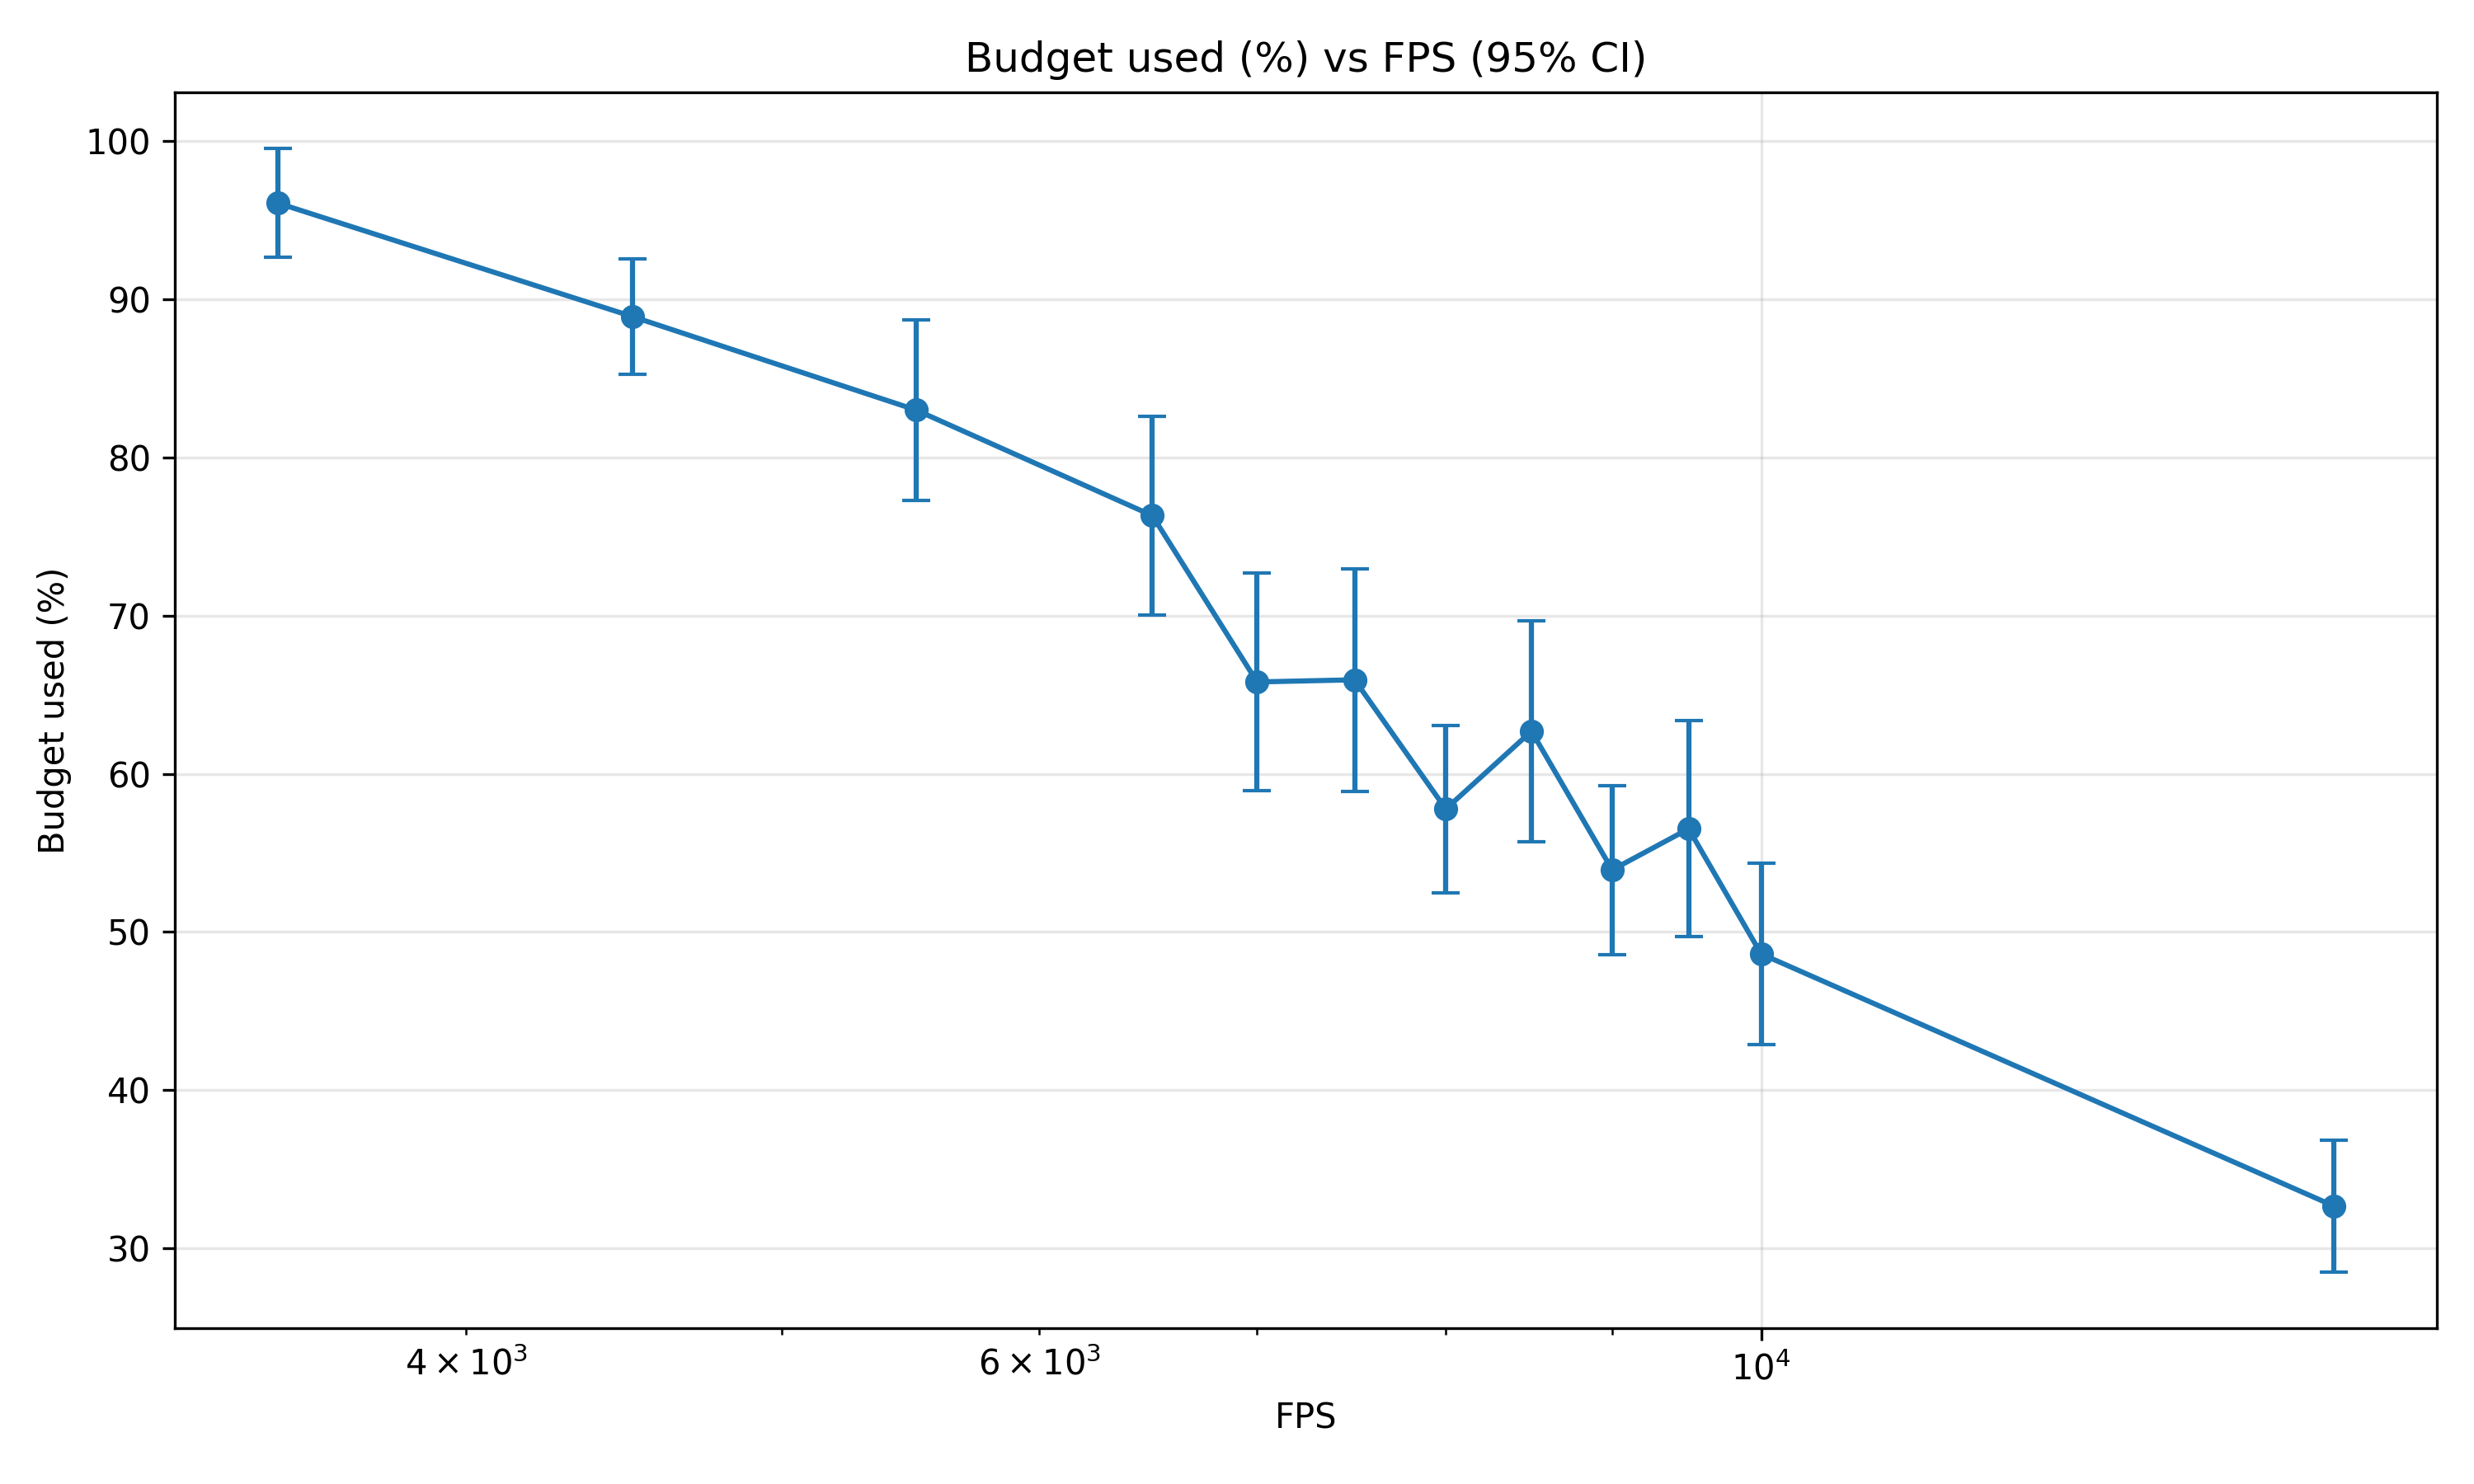
\includegraphics[width=1\textwidth]{travel_time_budget_used_ci95.png}
\caption{Budget used percentage for the travel-time-equity objective across sampled FPS values. Means and 95\% confidence intervals come from the 30-seed merged evaluation.}
\label{fig:travel_time_equity_subsidy_usage}
\end{figure}

\begin{figure}[!t]
\centering
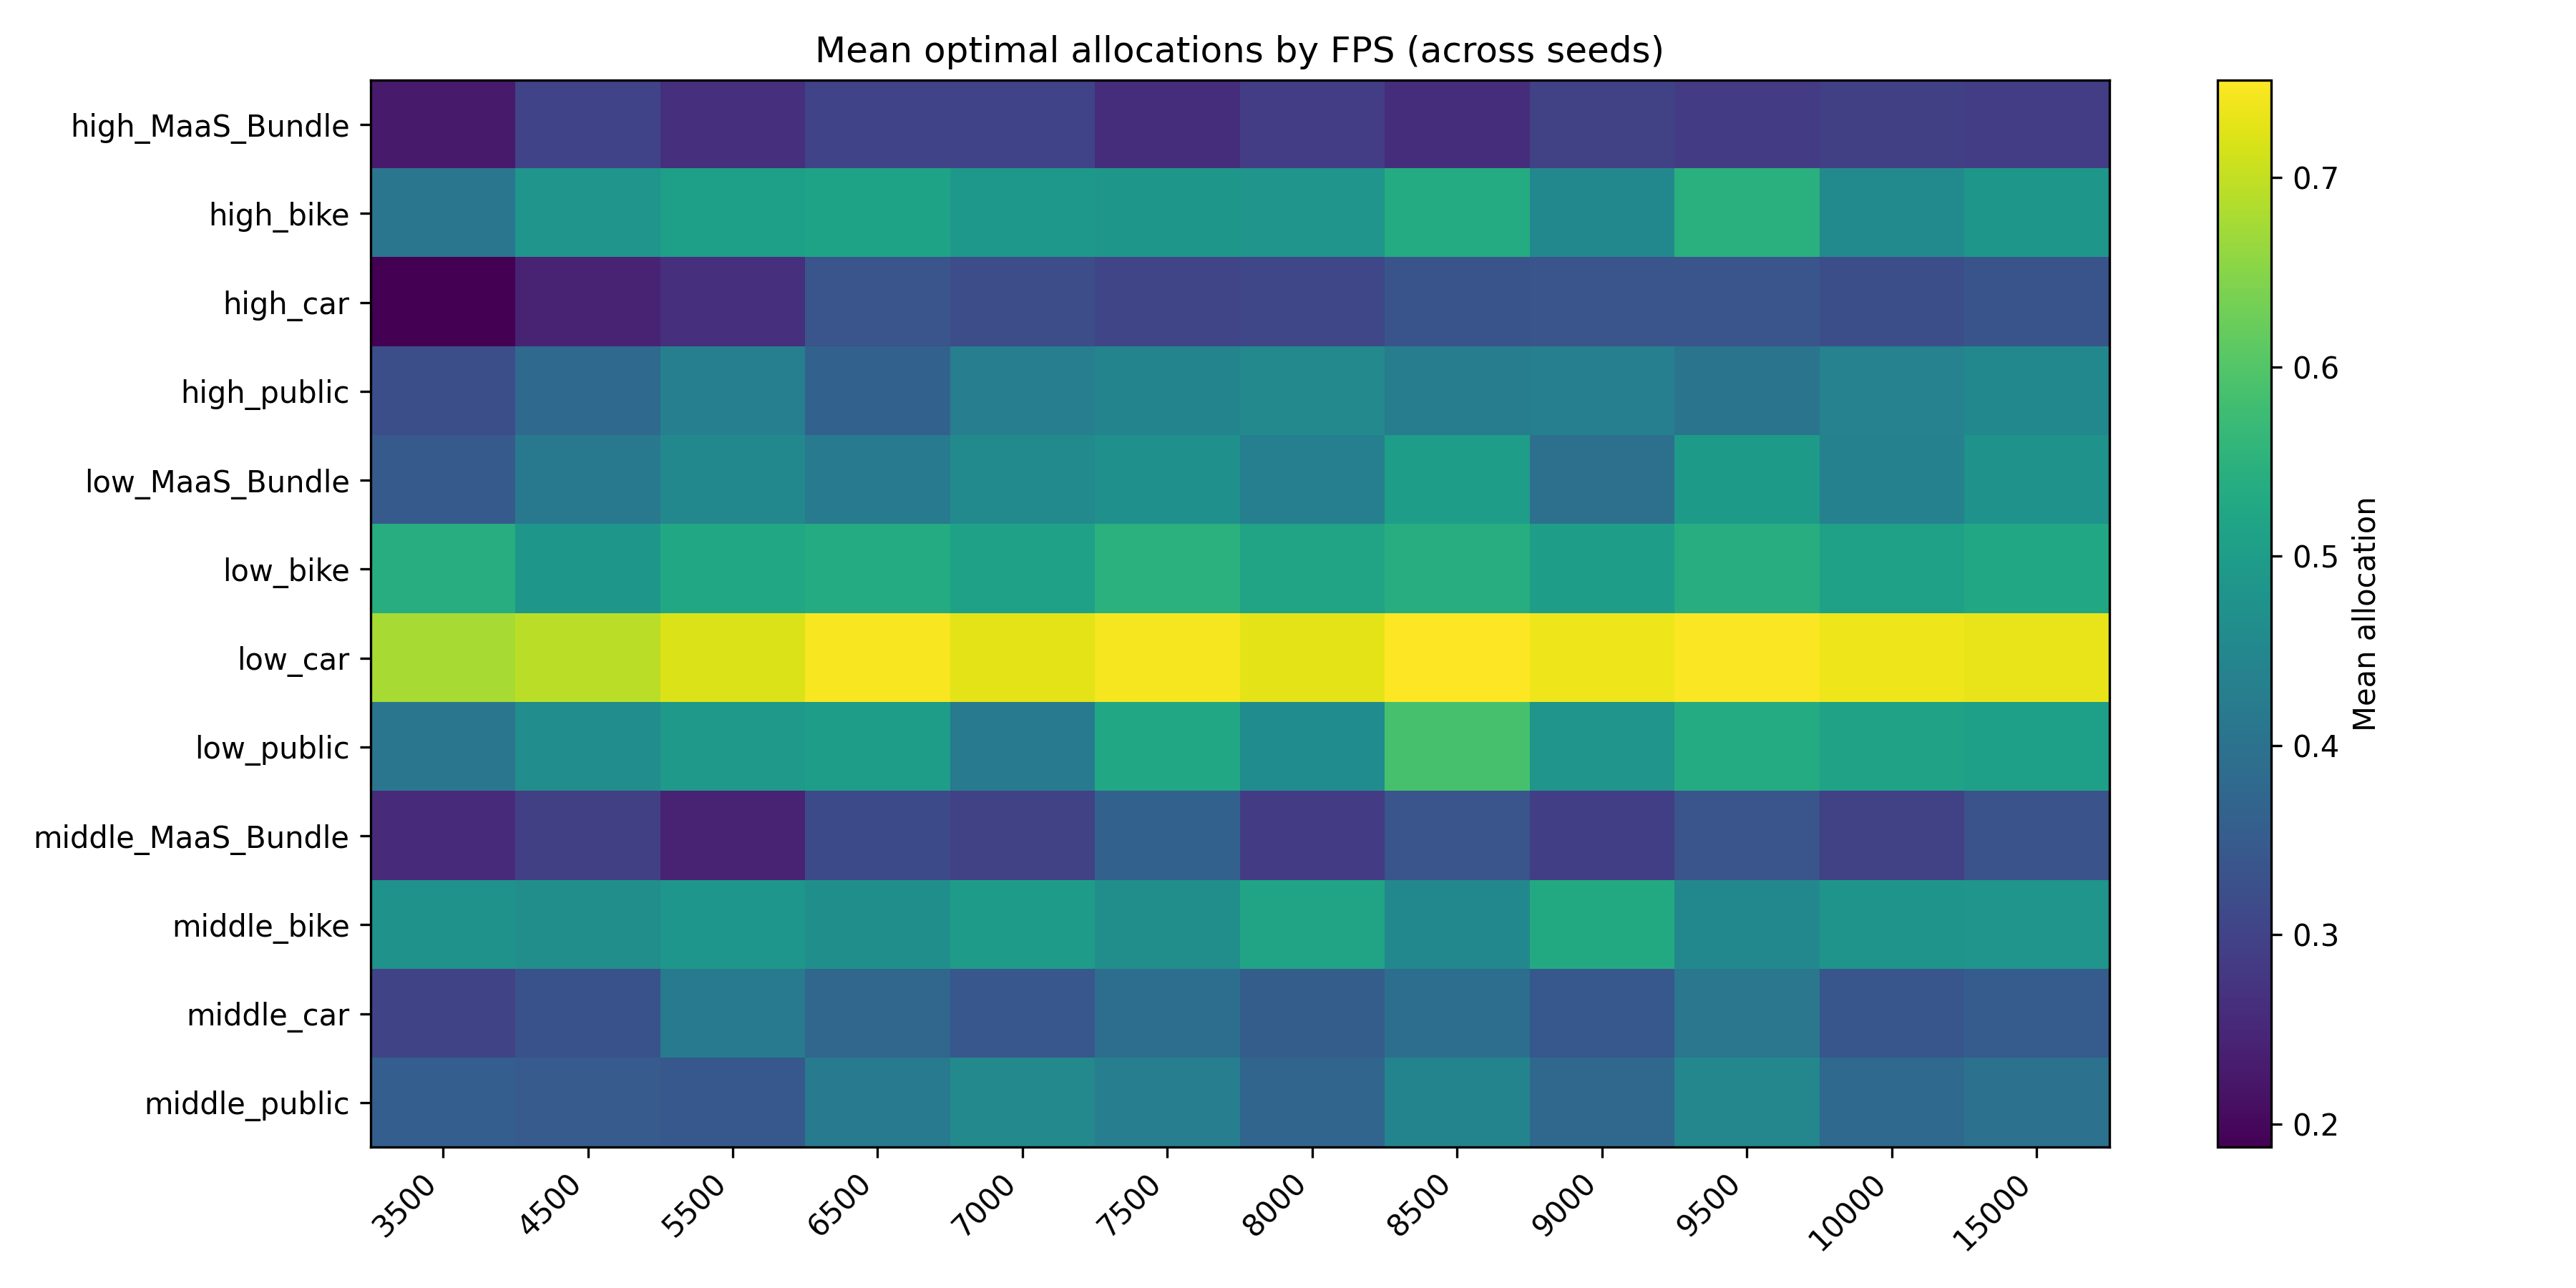
\includegraphics[width=0.9\textwidth]{travel_time_allocation_heatmap.png}
\caption{Mean subsidy-allocation heatmap for the travel-time-equity seed summary.}
\label{fig:travel_time_equity_relative_subsidy_distribution}
\end{figure}

As with mode-share equity, travel-time equity does not improve smoothly with every FPS increment. The deterministic fixed-policy control therefore matters for interpretation: once random demand and background conditions are held fixed, the objective improves monotonically or near-monotonically until realised subsidies saturate. We treat the stochastic irregularity in Figure~\ref{fig:travel_time_equity_FPS} as expected behaviour in a stochastic ABM rather than as a sign that the optimisation logic is invalid.

\subsection{Total System Travel Time Analysis}

\subsubsection{Optimisation Approach and Results}
\begin{figure}[!t]
\centering
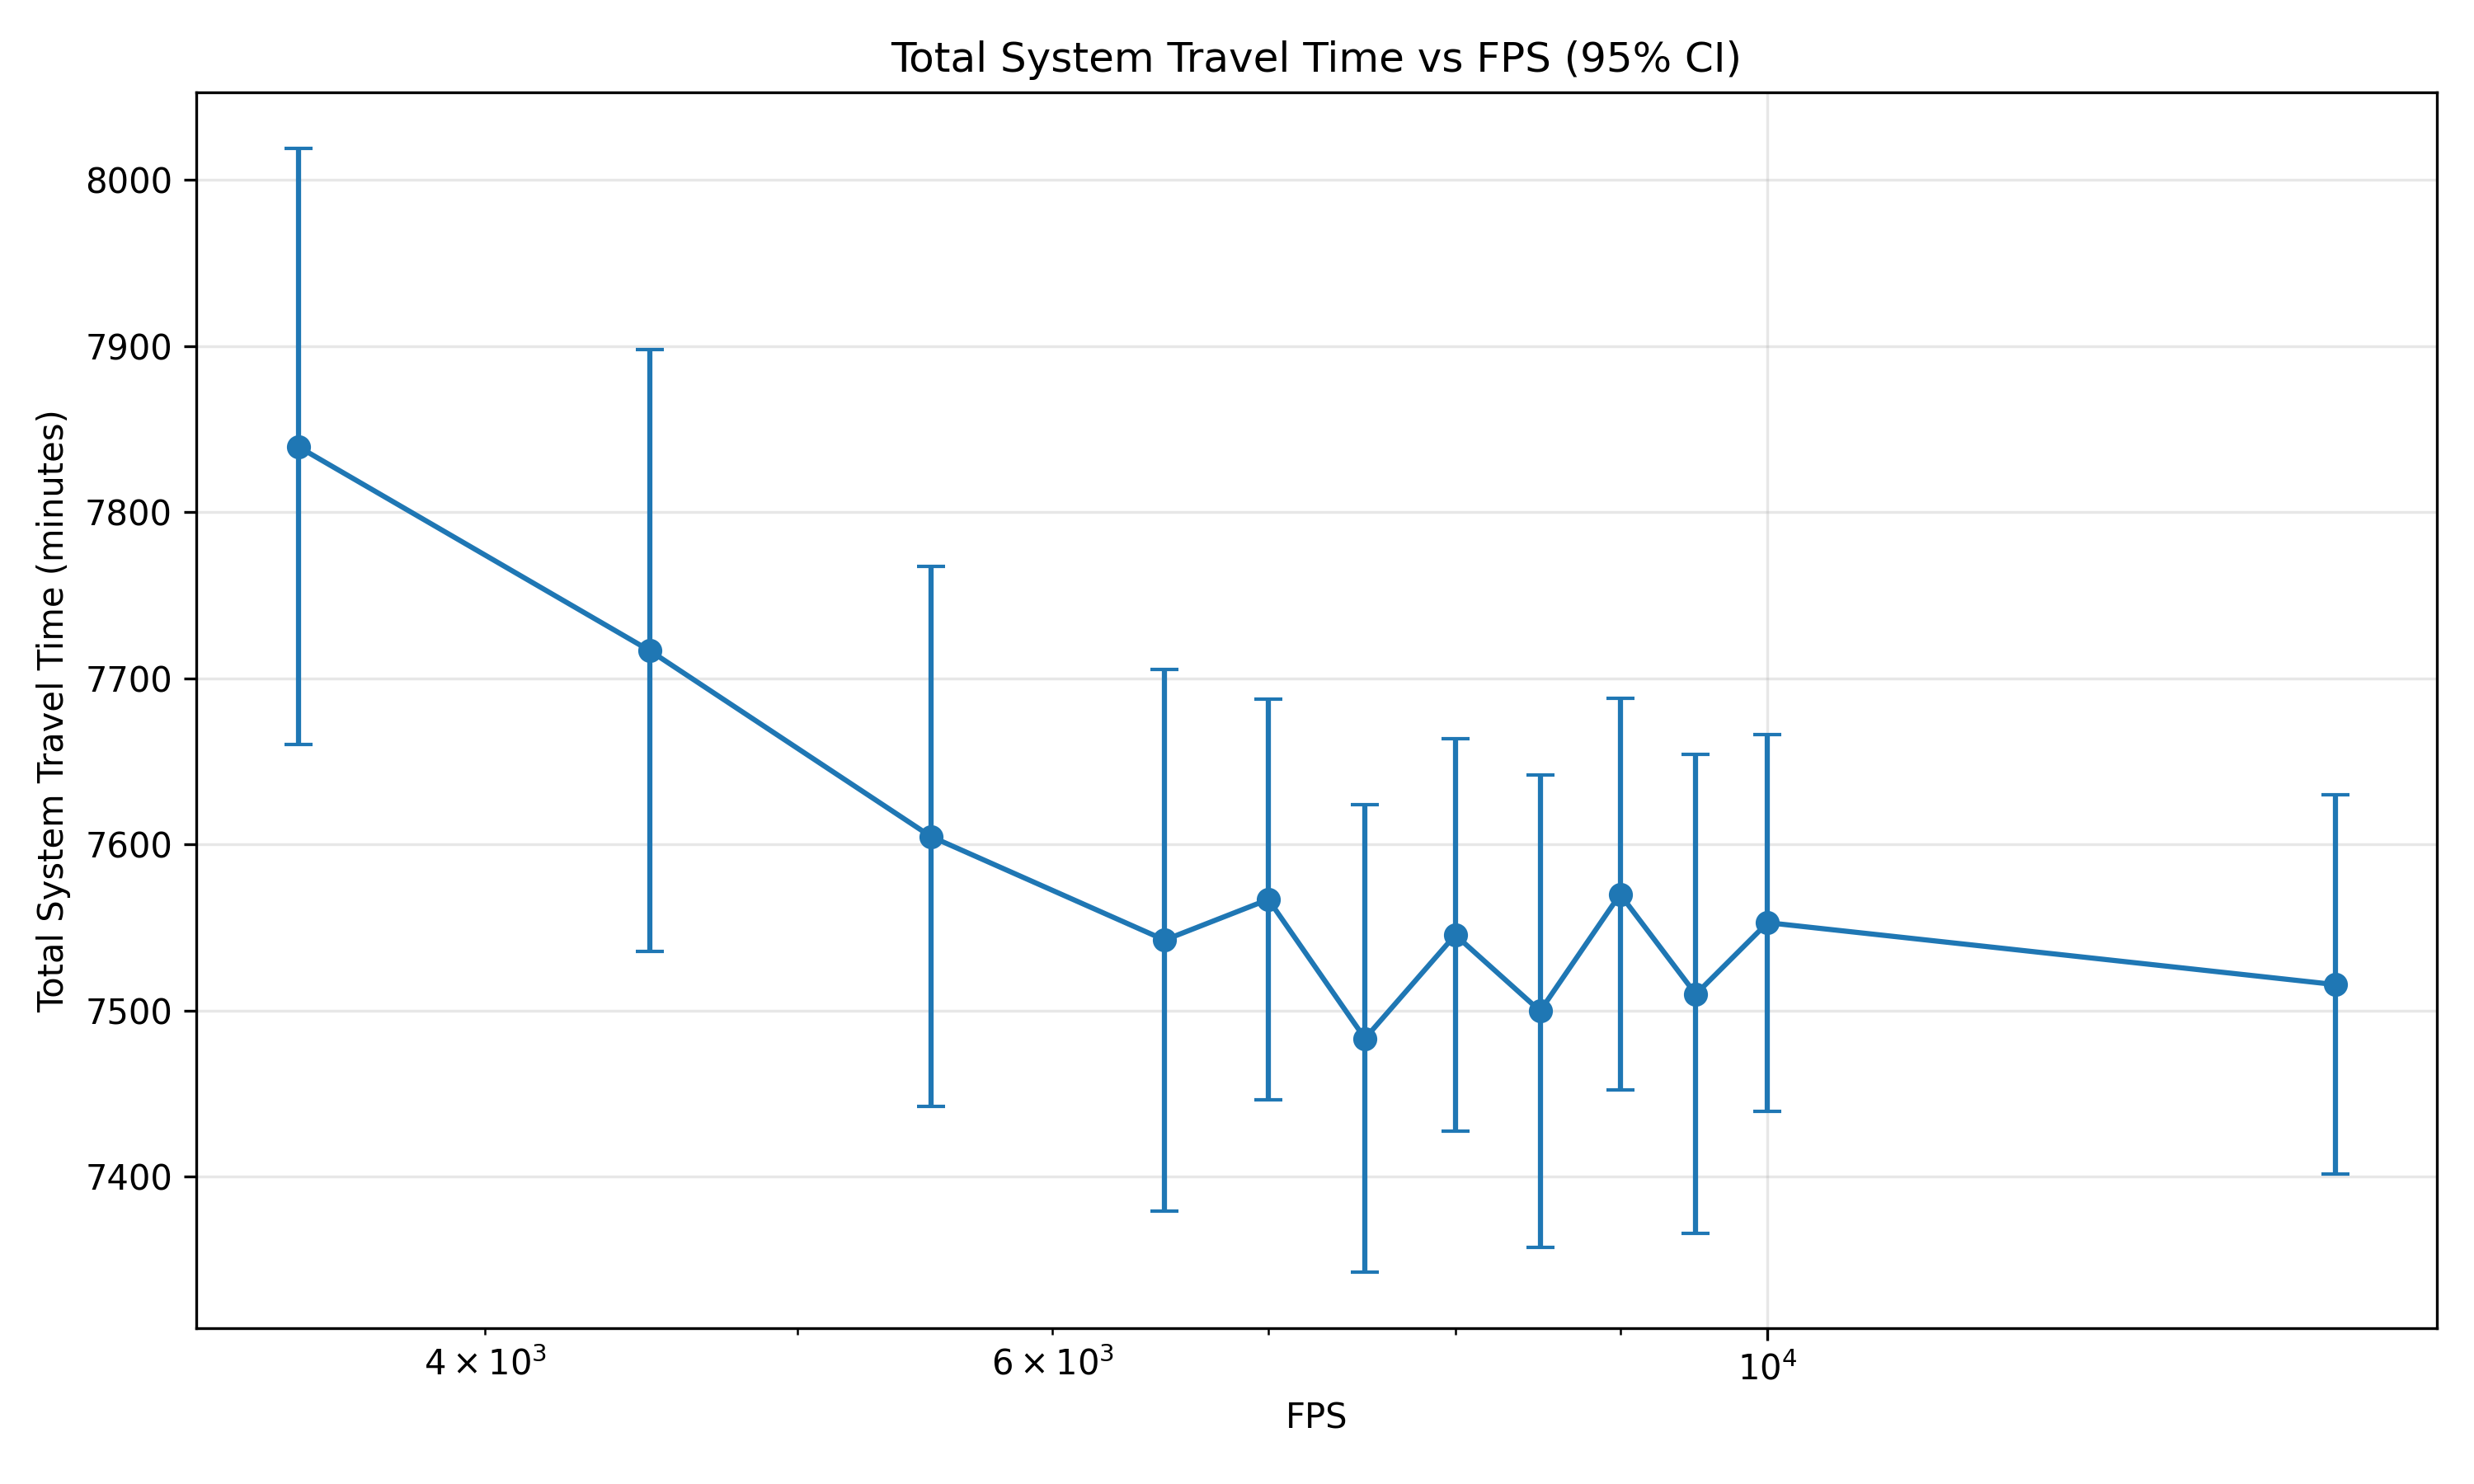
\includegraphics[width=1\textwidth]{tstt_ci95.png}
\caption{Total system travel time by FPS from the 30-seed merged evaluation. Means and 95\% confidence intervals are shown for each sampled FPS value. The lowest mean occurs at FPS 7,500, but much of the higher-FPS range remains on a broad plateau.}
\label{fig:total_travel_time}
\end{figure}
\begin{figure}[!t]
\centering
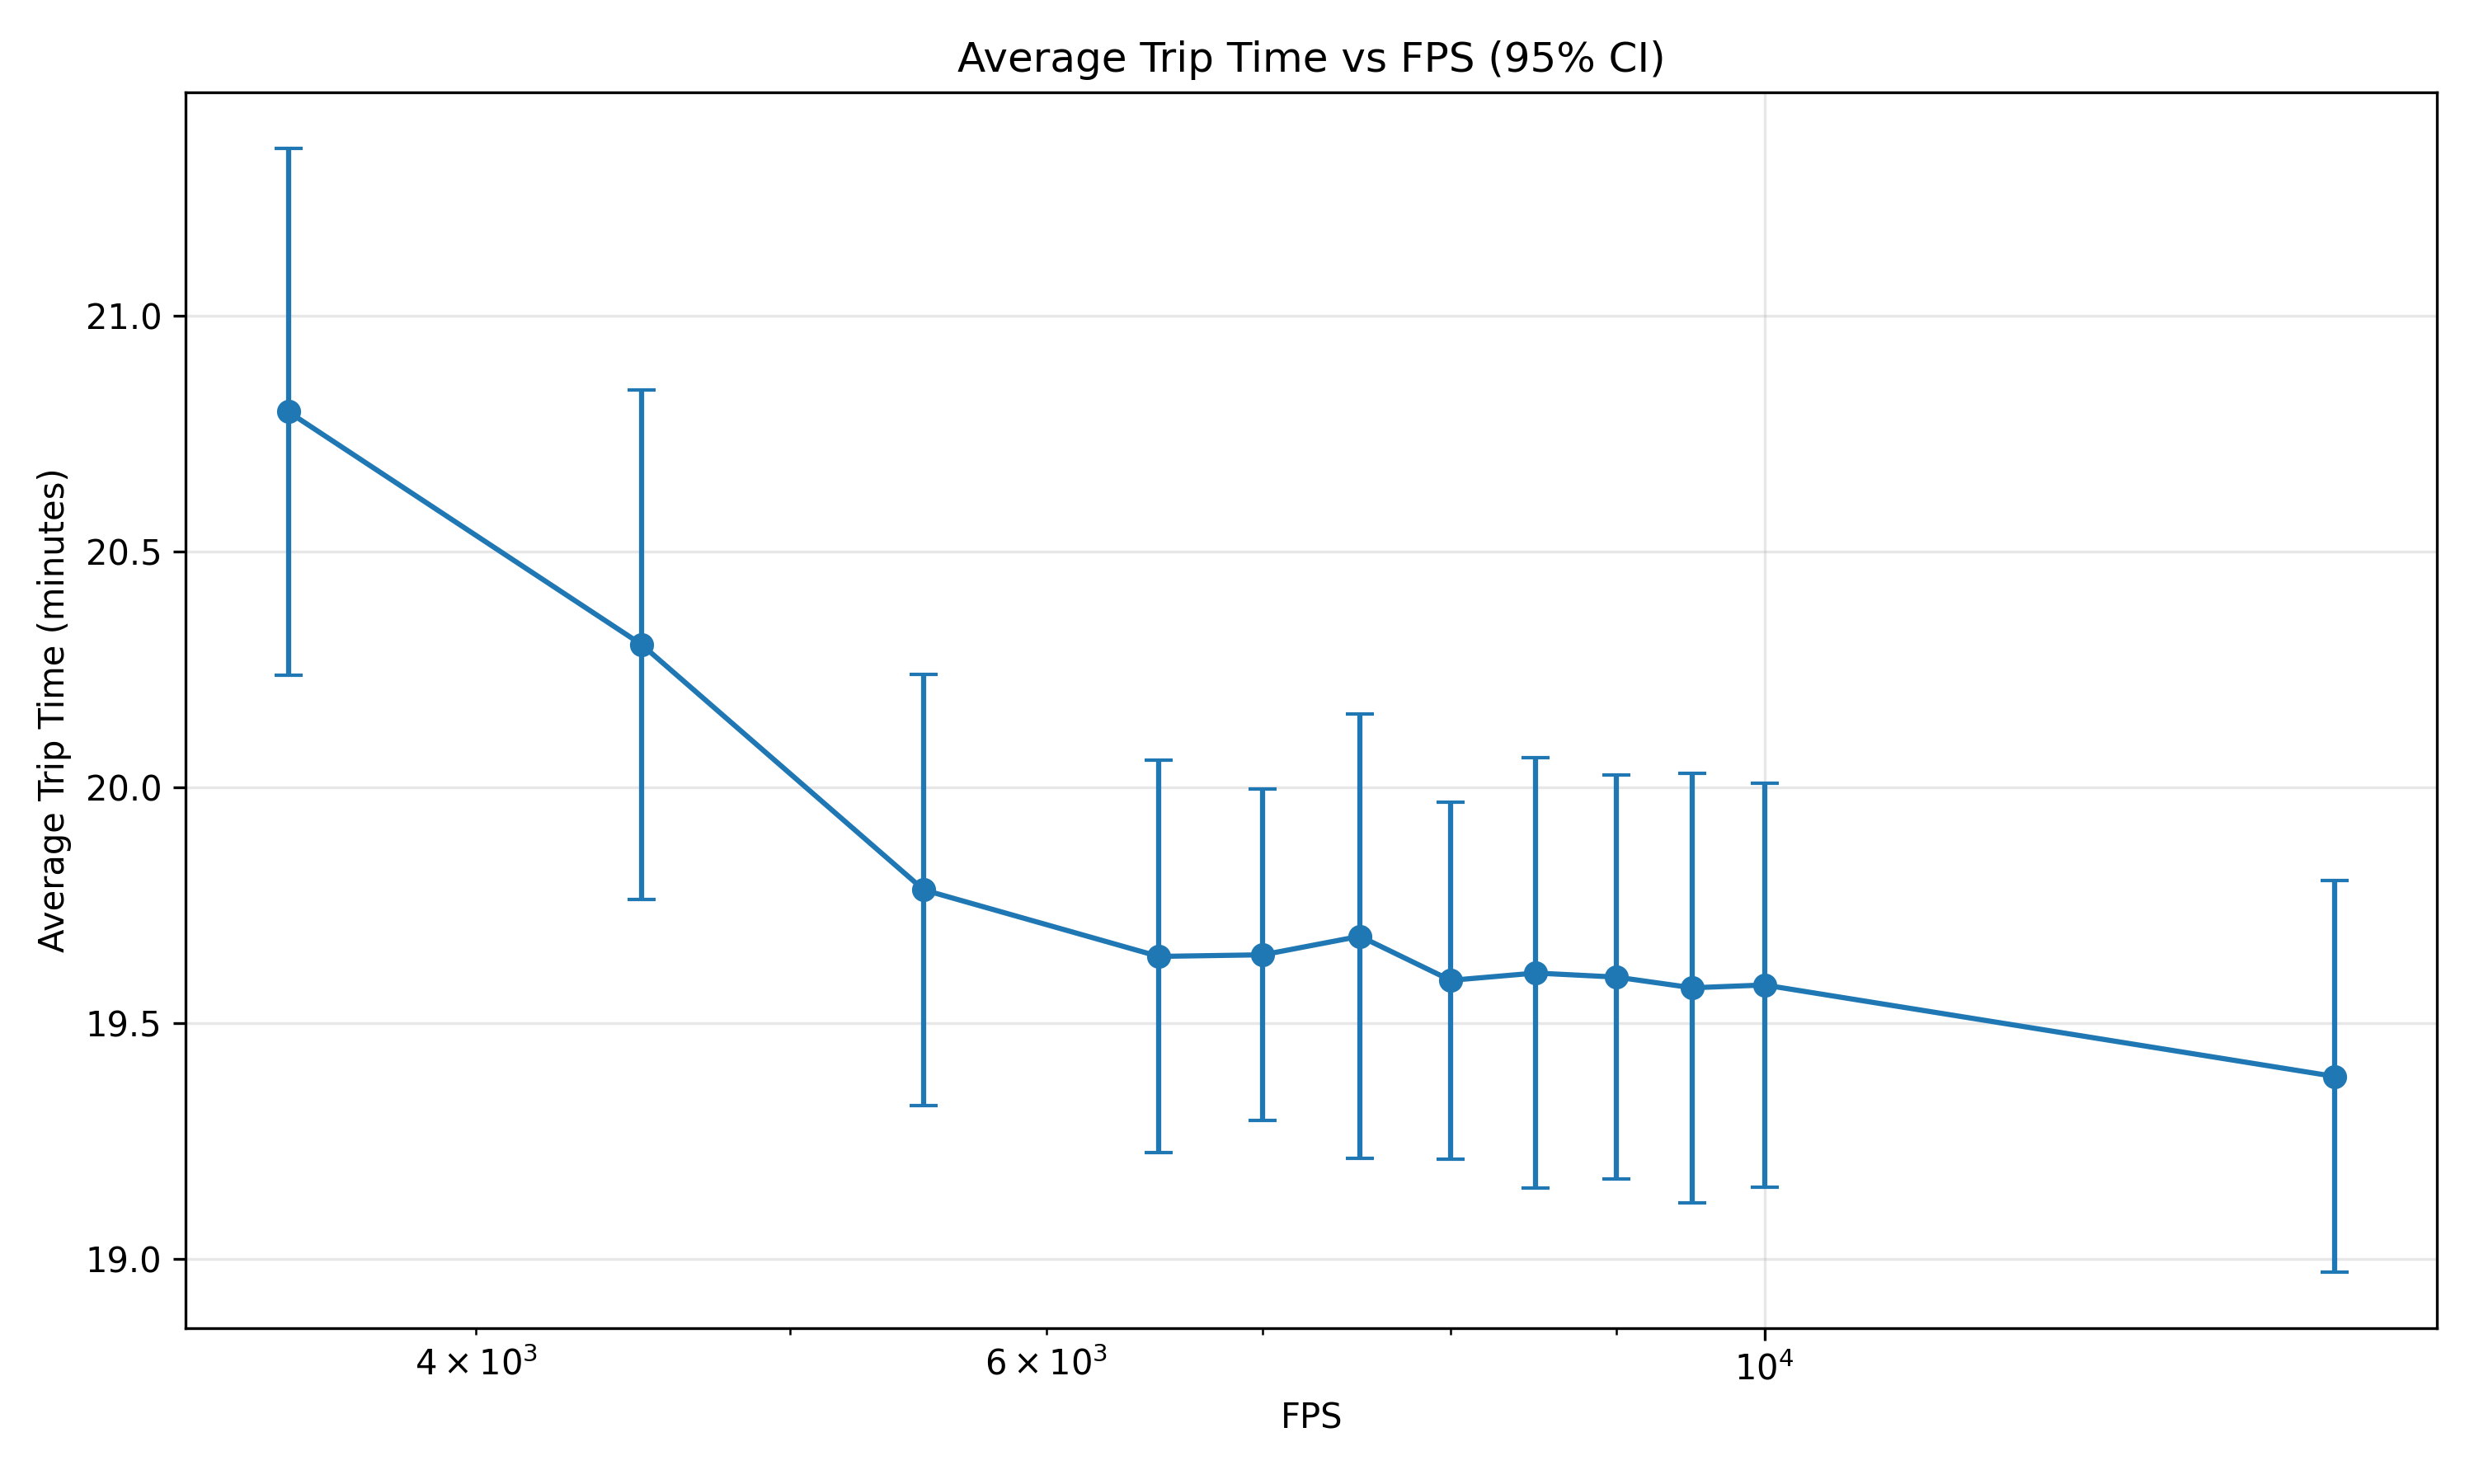
\includegraphics[width=1\textwidth]{tstt_avg_trip_time_ci95.png}
\caption{Average trip time by FPS from the 30-seed merged evaluation. Means and 95\% confidence intervals show that the total-system results are driven by moderate changes in trip time rather than by a sharp discontinuity.}
\label{fig:total_travel_time_by_income}
\end{figure}

\noindent The best mean total system travel time occurs at FPS 7,500 with $T_{\text{total}} = 7{,}483.23 \pm 140.75$ minutes (95\% CI, $n=30$). However, the regenerated cross-policy table classifies this objective as a broad plateau, because much of the range from FPS 4,500 to 15,000 remains close to the minimum in absolute terms. Budget usage at FPS 7,500 is lower than for the two equity objectives, at $58.61\% \pm 7.30$ percentage points.

The trip summary helps interpret this objective. Across the sampled FPS values, the mean total-trip count varies only from 377.4 to 388.3 trips, while mean trip time varies from 20.80 to 19.39 minutes. At FPS 7,500, the mean trip count is 380.7 and the mean trip time is 19.68 minutes. This suggests that the efficiency gains in the revised seed-based analysis come from moderate reductions in time burdens and redistribution across trips rather than from a dramatic surge in trip generation.

The mean aggregate allocation shares at the 7,500 optimum are 39.40\% for low income, 32.20\% for middle income, and 28.41\% for high income. The largest mean components are low-income public transport (0.7115), middle-income MaaS bundle (0.6099), and high-income public transport (0.6120), indicating a different structure from the equity-driven optima.

\subsubsection{Implementation Efficiency and Income Distribution}
\begin{figure}[!t]
\centering
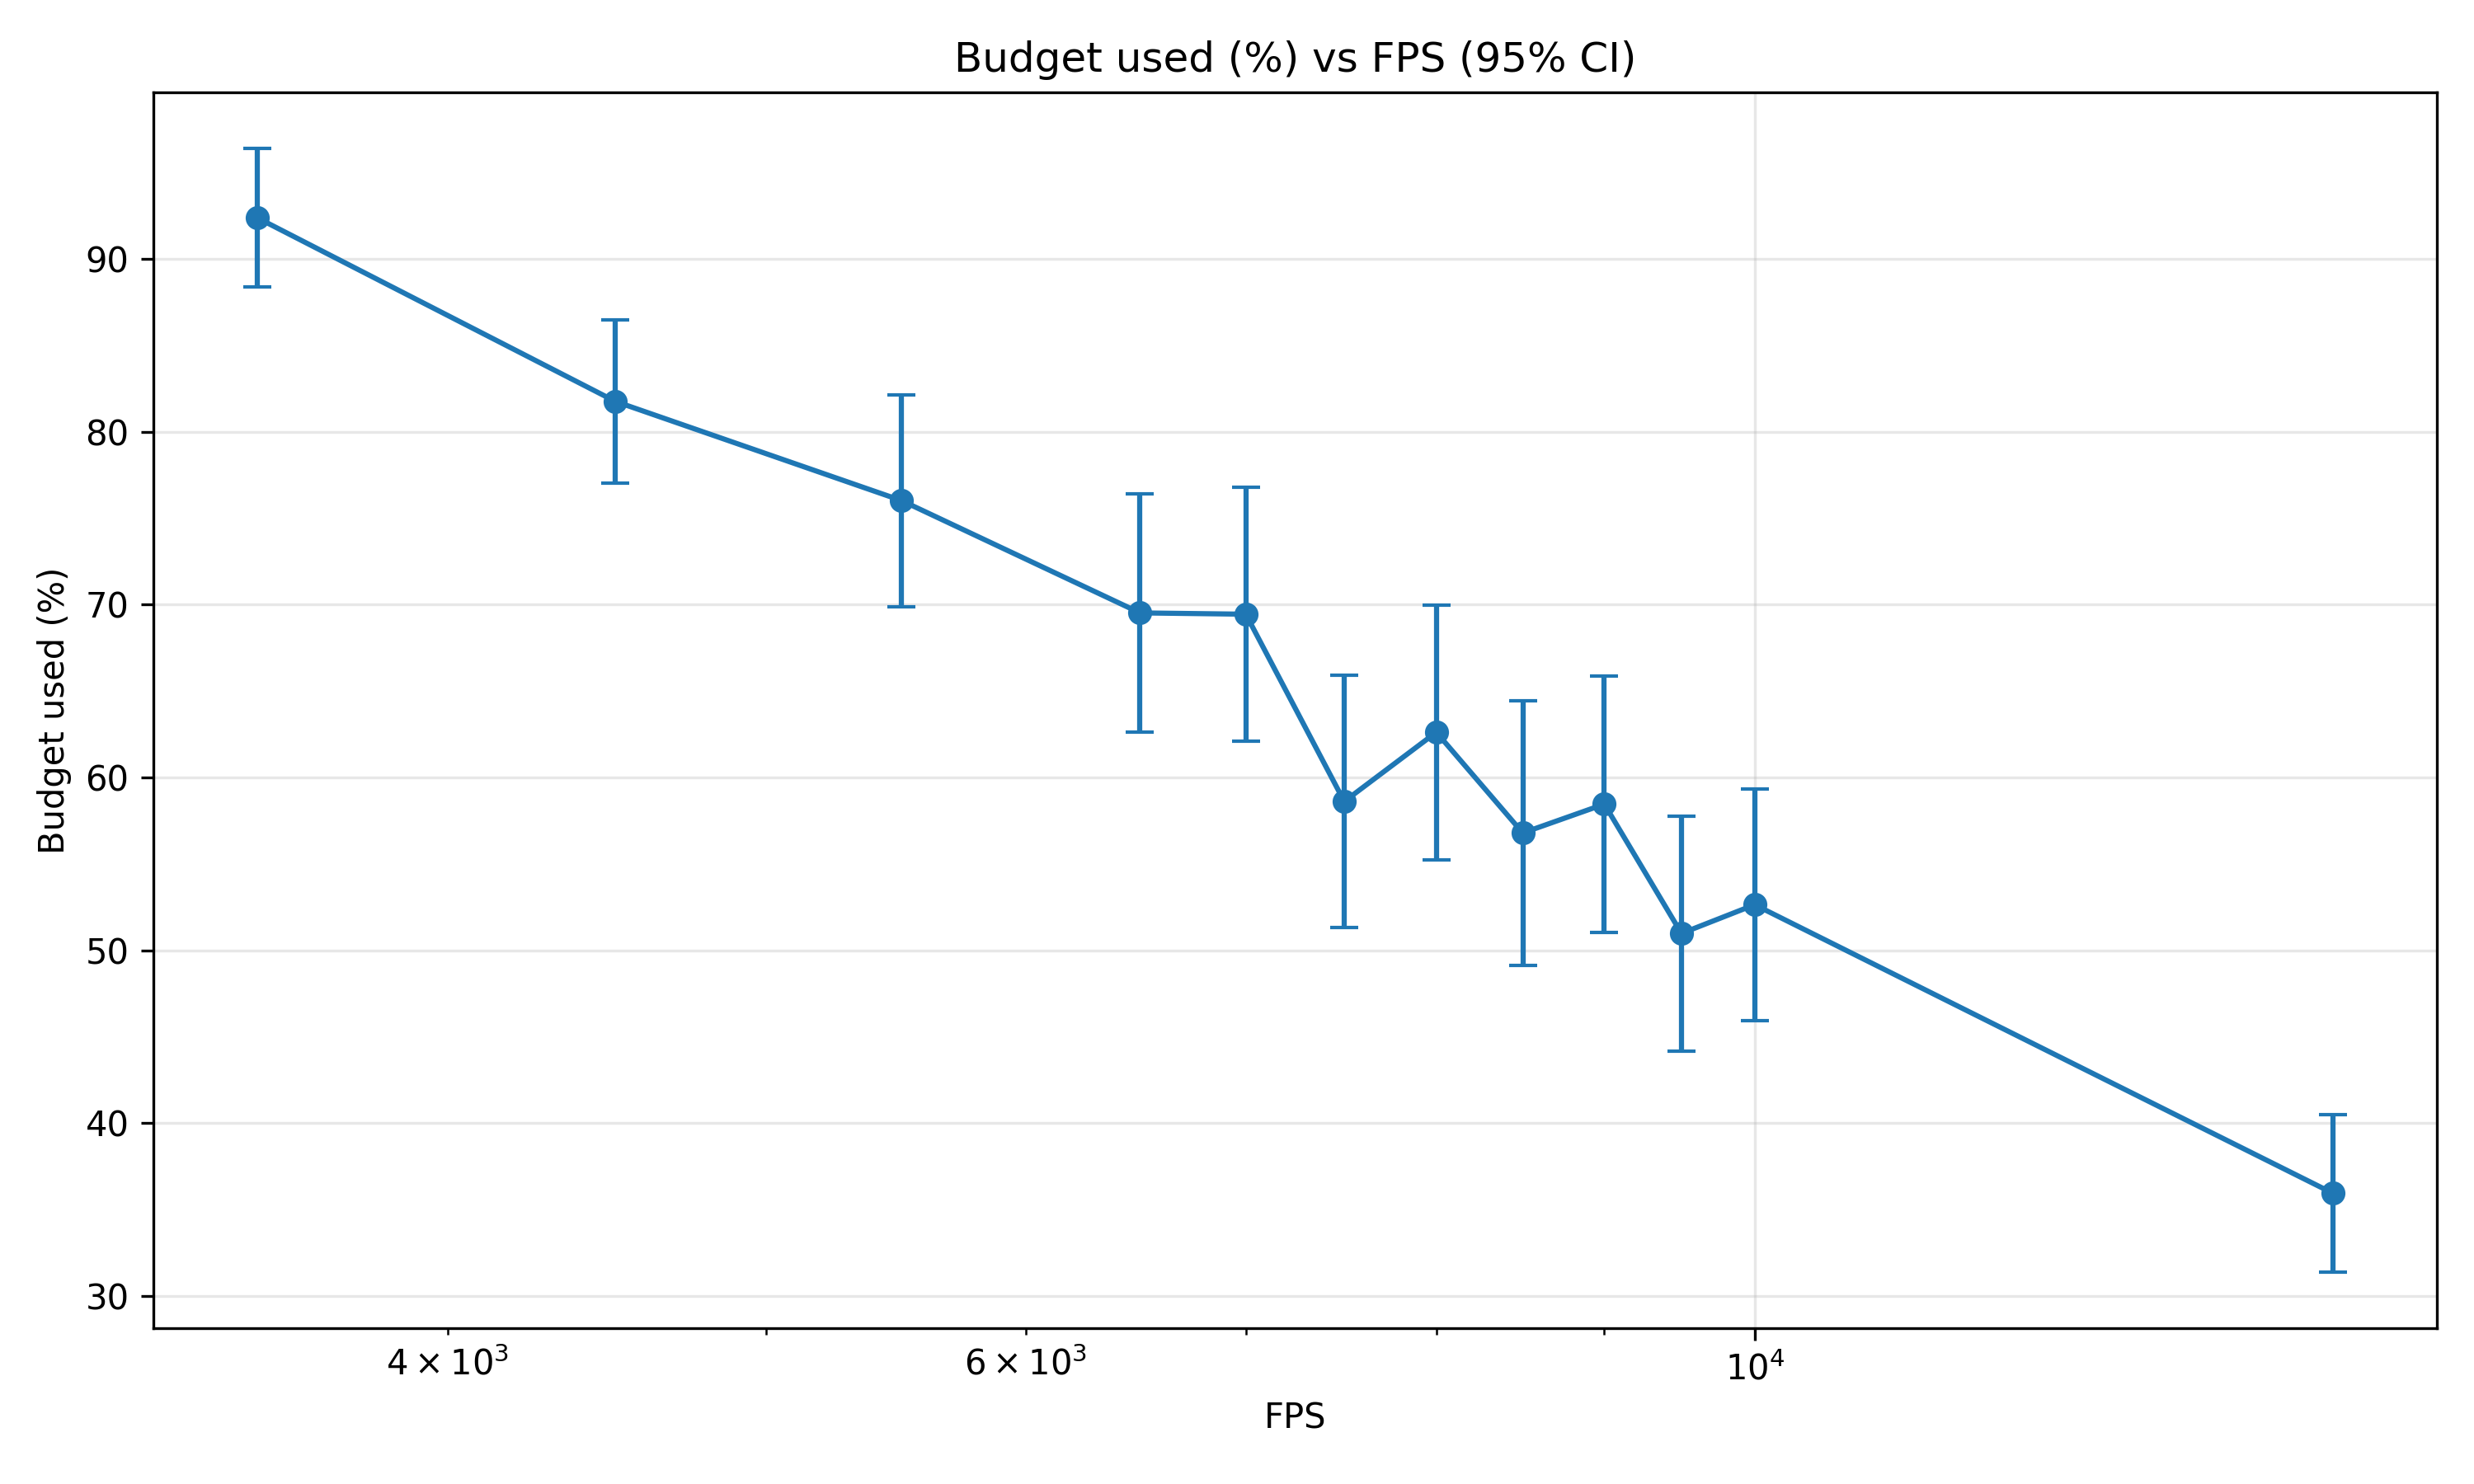
\includegraphics[width=1\textwidth]{tstt_budget_used_ci95.png}
\caption{Budget used percentage for the total-system-travel-time objective across sampled FPS values. Means and 95\% confidence intervals come from the 30-seed merged evaluation.}
\label{fig:total_travel_time_subsidy_usage}
\end{figure}
\begin{figure}[!t]
\centering
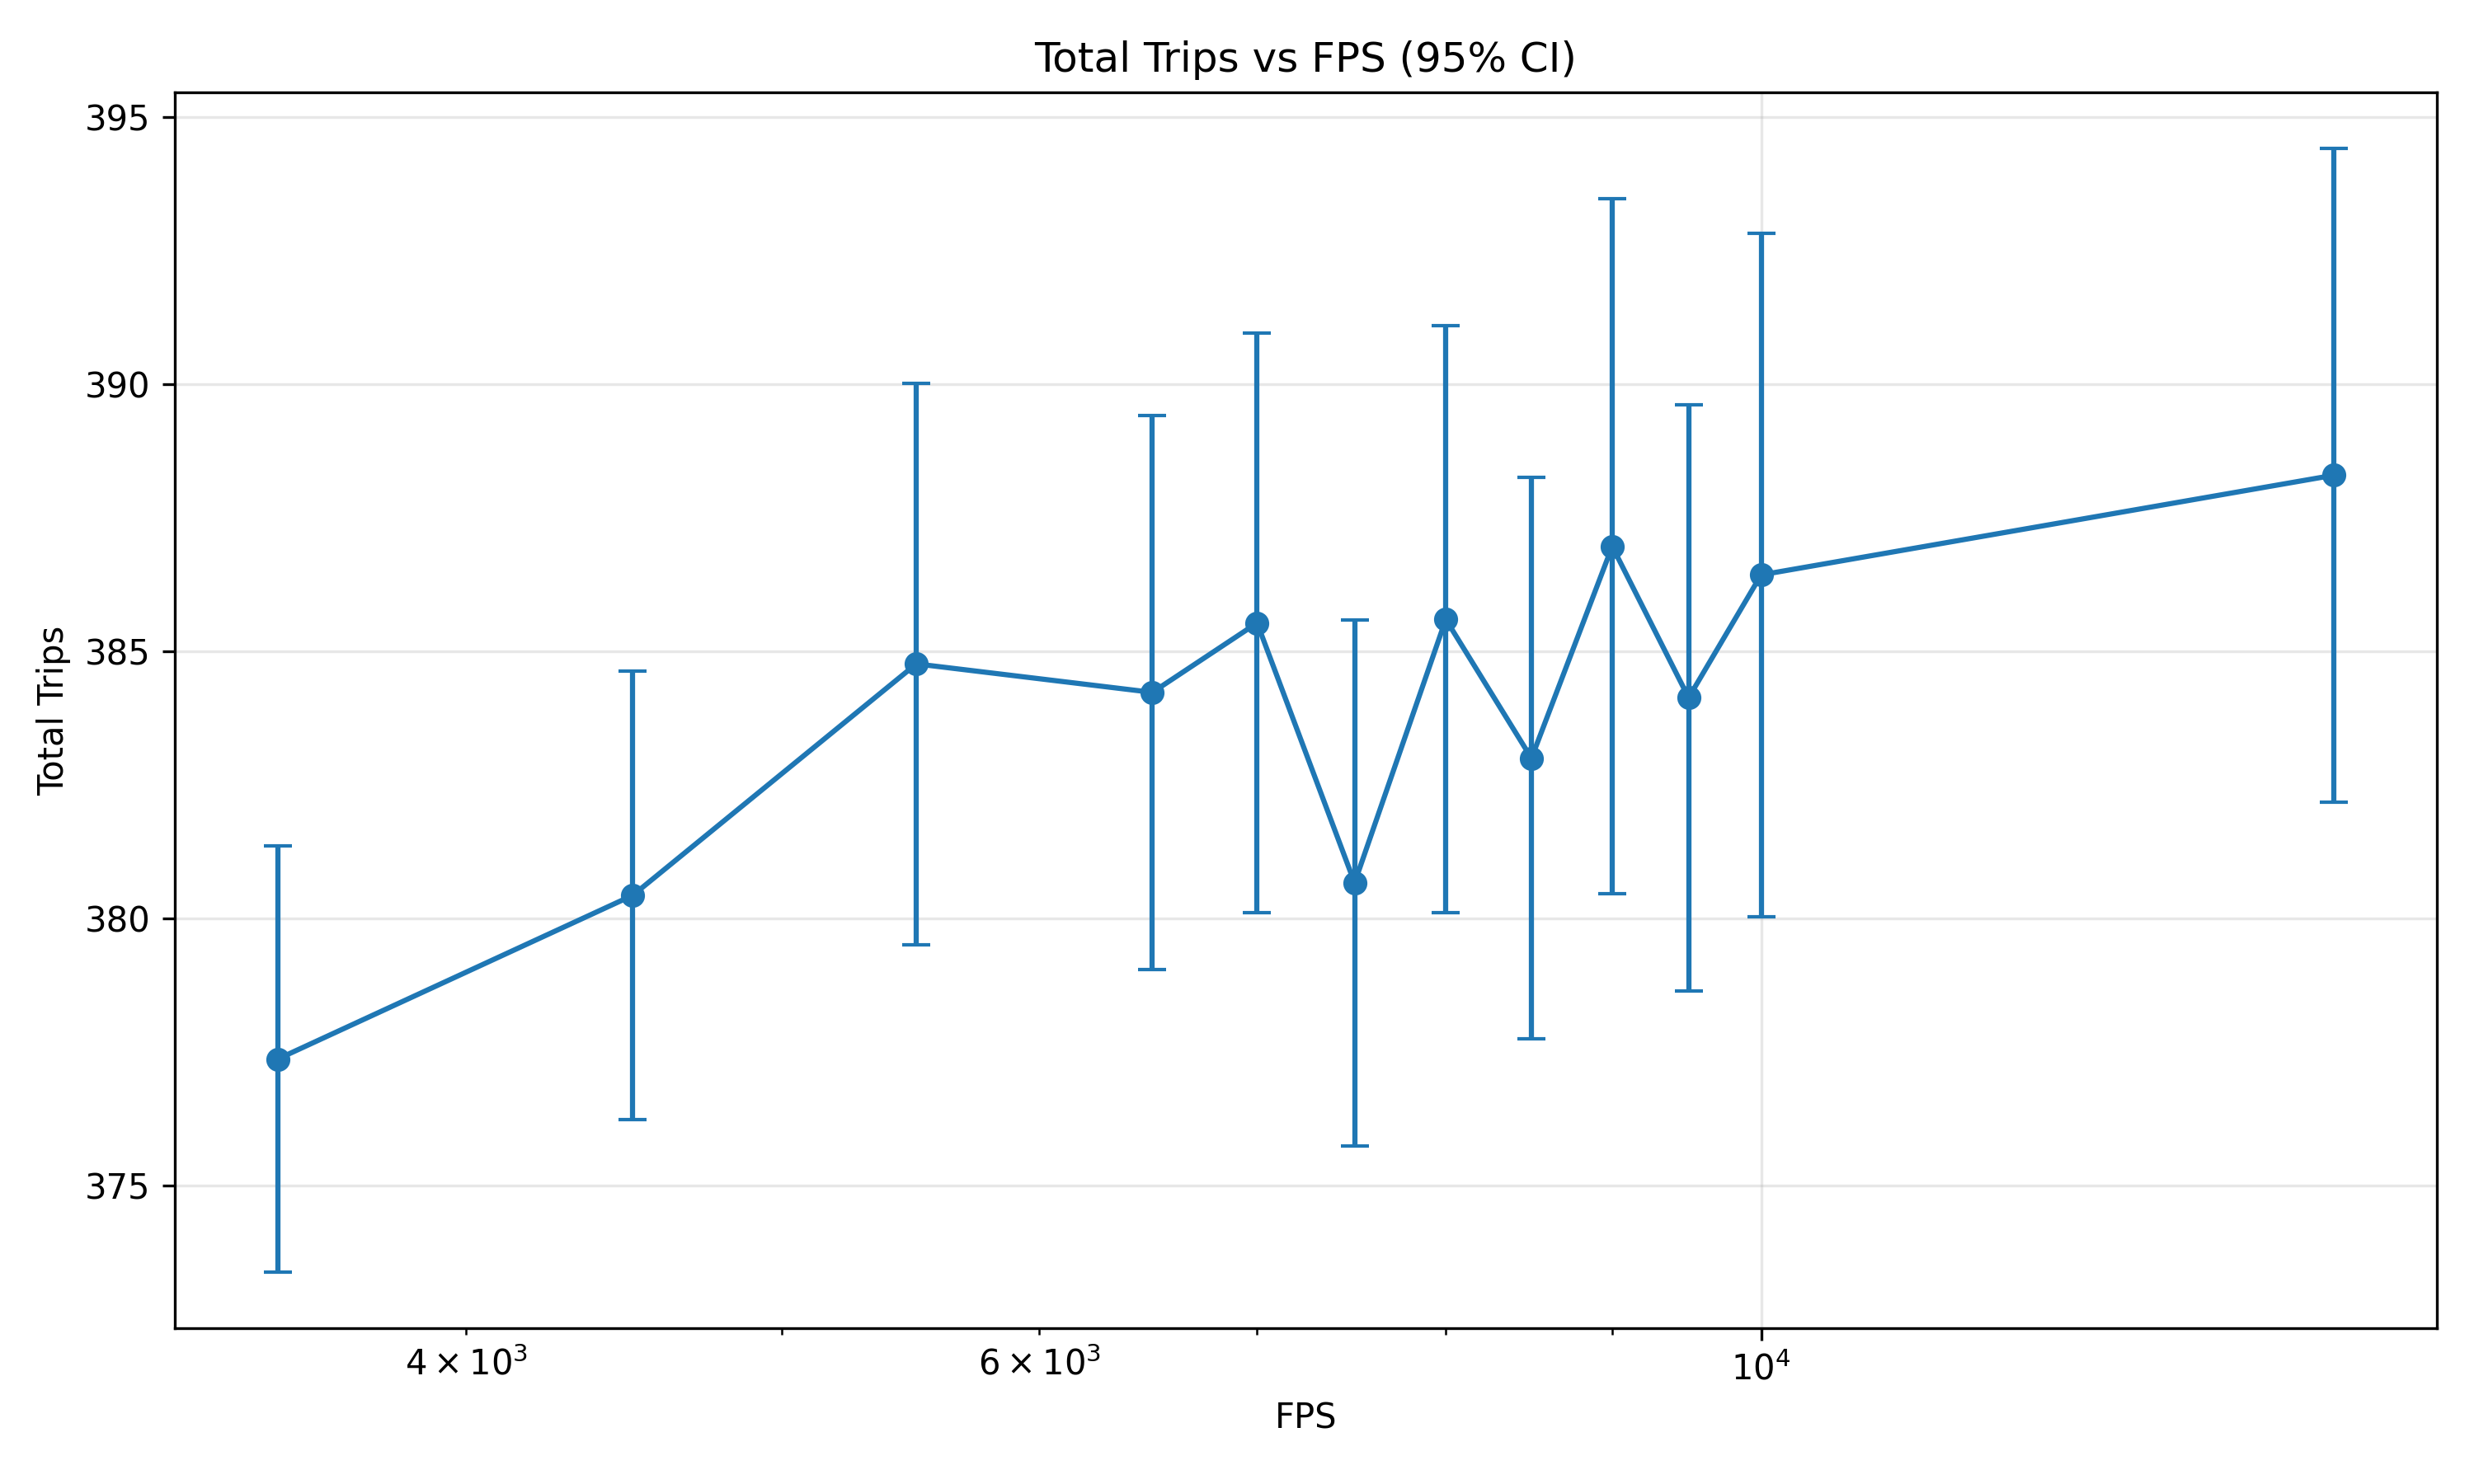
\includegraphics[width=1\textwidth]{tstt_total_trips_ci95.png}
\caption{Total trips by FPS from the 30-seed merged evaluation. The relative stability of trip counts helps explain why the total-system objective forms a shallow plateau rather than a single narrow optimum.}
\label{fig:total_travel_time_subsidy_distribution}
\end{figure}

The total-system objective exhibits the clearest saturation pattern: policy performance remains broadly competitive even while the share of the budget that is actually used falls at higher FPS values. This explains why the revised cross-policy guidance treats efficiency as a plateau problem rather than as a sharp optimum problem.

\section{Cross-Policy Synthesis}\label{sec:synthesis}

\subsection{Comparative Analysis of Policy Approaches}

\begin{figure}[!t]
\centering
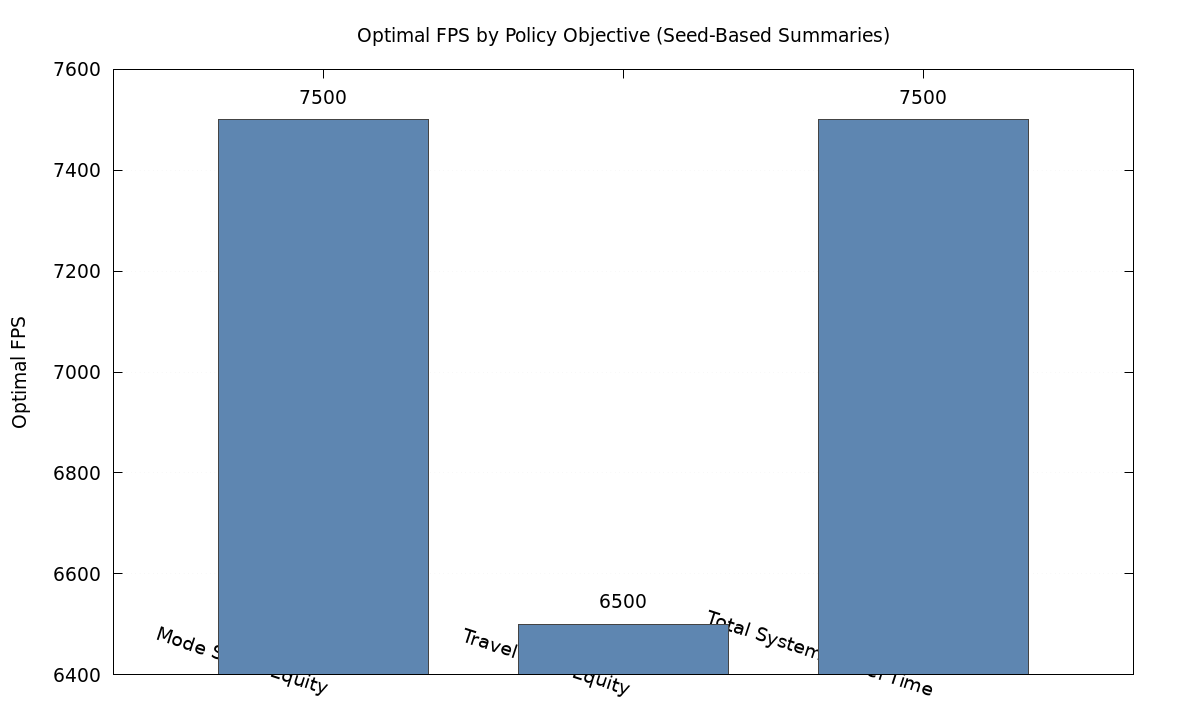
\includegraphics[width=0.8\textwidth]{cross_policy_optimal_fps_comparison.png}
\caption{Comparison of objective-specific optimal FPS values from the regenerated seed-based summaries. Error bars show 95\% confidence intervals around the objective mean at each objective-specific optimum.}
\label{fig:optimal_fps_comparison}
\end{figure}

\begin{figure}[!t]
\centering
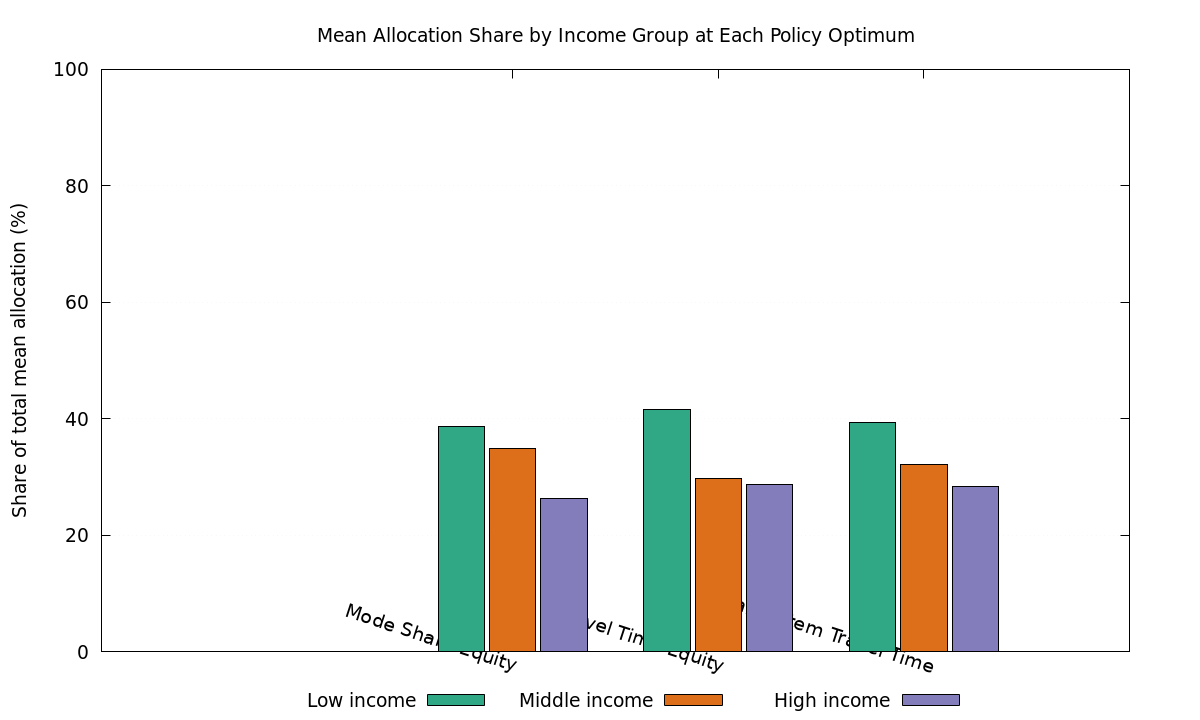
\includegraphics[width=0.8\textwidth]{cross_policy_income_shares.png}
\caption{Aggregate income-group allocation shares at the objective-specific optima from the regenerated seed-based summaries. The low-income group receives the largest share in all three cases, but the margins are much smaller than in the legacy single-run manuscript.}
\label{fig:cross_policy_income_distribution}
\end{figure}

\begin{figure}[!t]
\centering
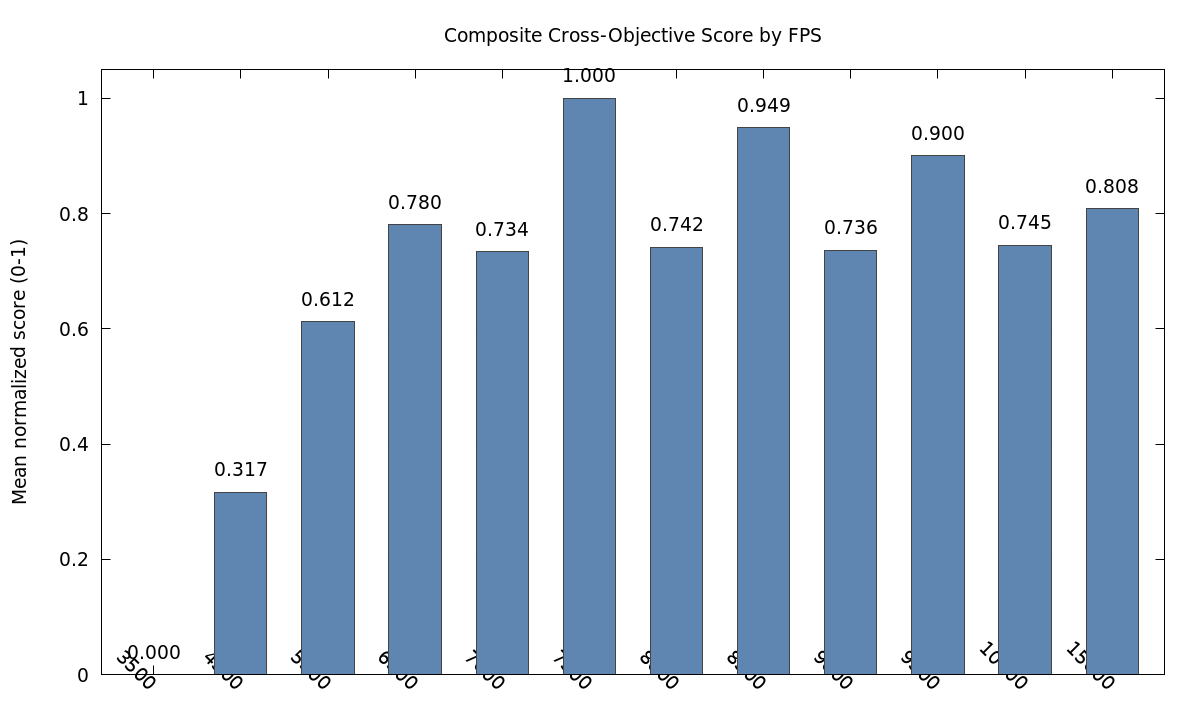
\includegraphics[width=0.8\textwidth]{cross_policy_performance_tradeoffs.png}
\caption{Regenerated cross-policy trade-off view using the current seed-based objective summaries.}
\label{fig:tradeoffs}
\end{figure}
\begin{figure}[!t]
\centering
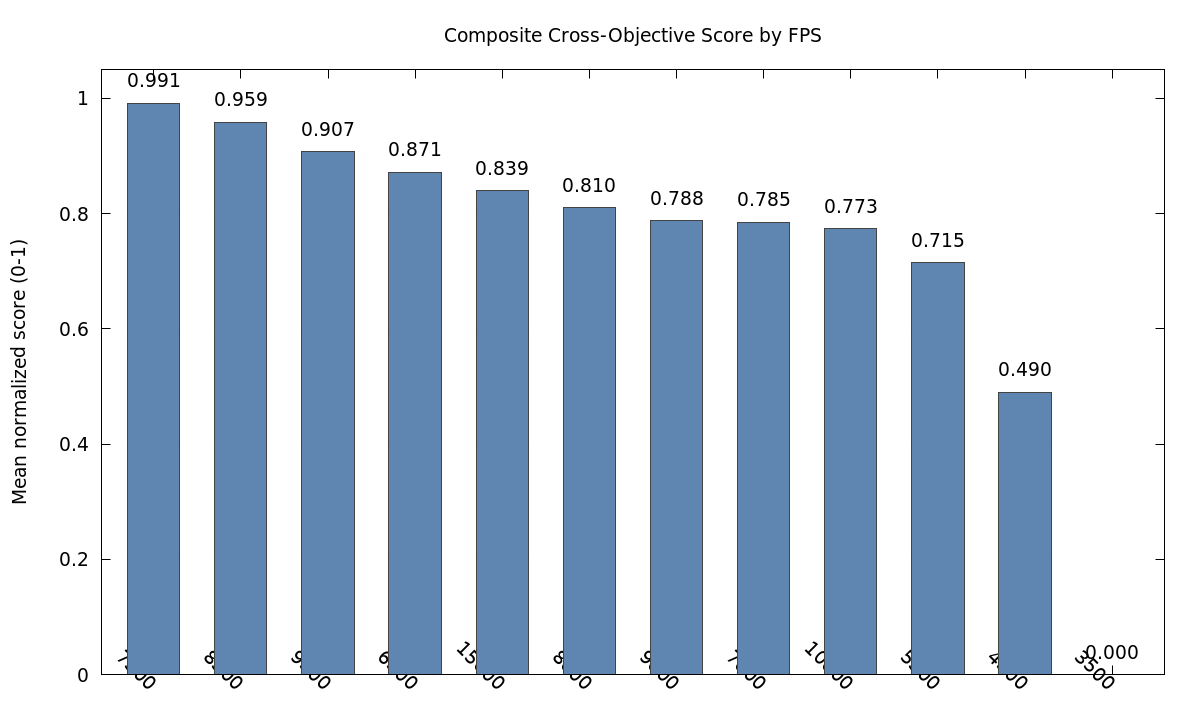
\includegraphics[width=1\textwidth]{cross_policy_composite_ranking.png}
\caption{Composite cross-objective ranking across the common sampled FPS values after normalising each objective to a decision-support scale. FPS 7,500 ranks first in the regenerated comparison.}
\label{fig:multi_objective}
\end{figure}

\begin{figure}[!t]
\centering

\includegraphics[width=1\textwidth]{cross_policy_decision_support.png}
\caption{Regenerated decision-support framework derived from the current seed-based summaries.}
\label{fig:recommendations}
\end{figure}

The regenerated cross-policy comparison is materially different from the legacy single-run manuscript. The seed-mean optima occur at FPS 7,500 for mode-share equity, FPS 6,500 for travel-time equity, and FPS 7,500 for total system travel time (Figure~\ref{fig:optimal_fps_comparison}). This places the three objectives much closer together than the earlier 4,000--5,000 narrative implied, although the efficiency objective remains flatter than the two equity objectives.

The aggregate allocation shares at the objective-specific optima also change substantially. Low-income travellers receive the largest share in all three objectives, but the observed shares are 38.74\%, 41.57\%, and 39.40\% rather than the much steeper 55--65\% pattern reported previously. We therefore describe the revised evidence more carefully: within this stylised scenario, the optimiser often favours low-income travellers, but it does so through mixed allocations that still leave large roles for middle-income and high-income cells. This avoids overstating a universal progressive rule.

Among the common sampled FPS values, the regenerated composite ranking places FPS 7,500 first, followed by 8,500, 9,500, and 6,500 (Figure~\ref{fig:multi_objective}). This normalised ranking is presented only as a decision-support device for comparing heterogeneous metrics; it is not a claim that the raw metrics share a common natural scale. The revised cross-policy conclusion is therefore scenario-specific: in the current synthetic environment, the seed-based optima do not show a large conflict between the two equity criteria and the efficiency criterion, but we do not claim this resolves the equity-efficiency debate in general \citep{Martens2016, Pereira2017, DiCiommo2017}. We also do not interpret a better equity score as proof of a Pareto improvement. In this framework, an equity metric can improve because disadvantaged users do better, because other users do worse, or because both move together. The cross-policy plots therefore make those trade-offs explicit rather than treating the objective-specific optima as universally beneficial for every group.
This distribution-sensitive framing is consistent with transport-equity scholarship that evaluates policies partly by how they shift opportunities toward disadvantaged groups rather than by equalising nominal benefits across all travellers \citep{Martens2016, Pereira2017, Lucas2016}.

\subsection{Subsidy Investment Guidance}
\begin{figure}[!t]
\centering
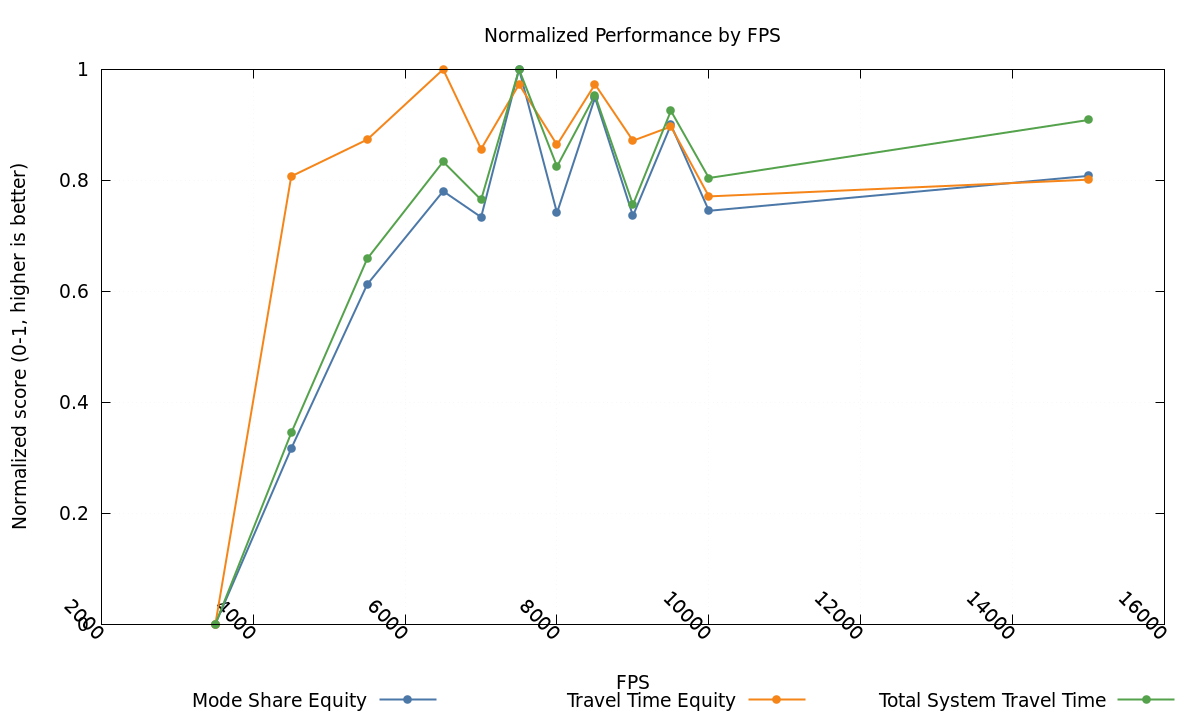
\includegraphics[width=1\textwidth]{cross_policy_normalized_performance.png}
\caption{Normalised policy-performance curves used for cross-objective decision support. The normalisation is applied only for comparison across heterogeneous metrics.}
\label{fig:dim_returns}
\end{figure}
\begin{figure}[!t]
\centering
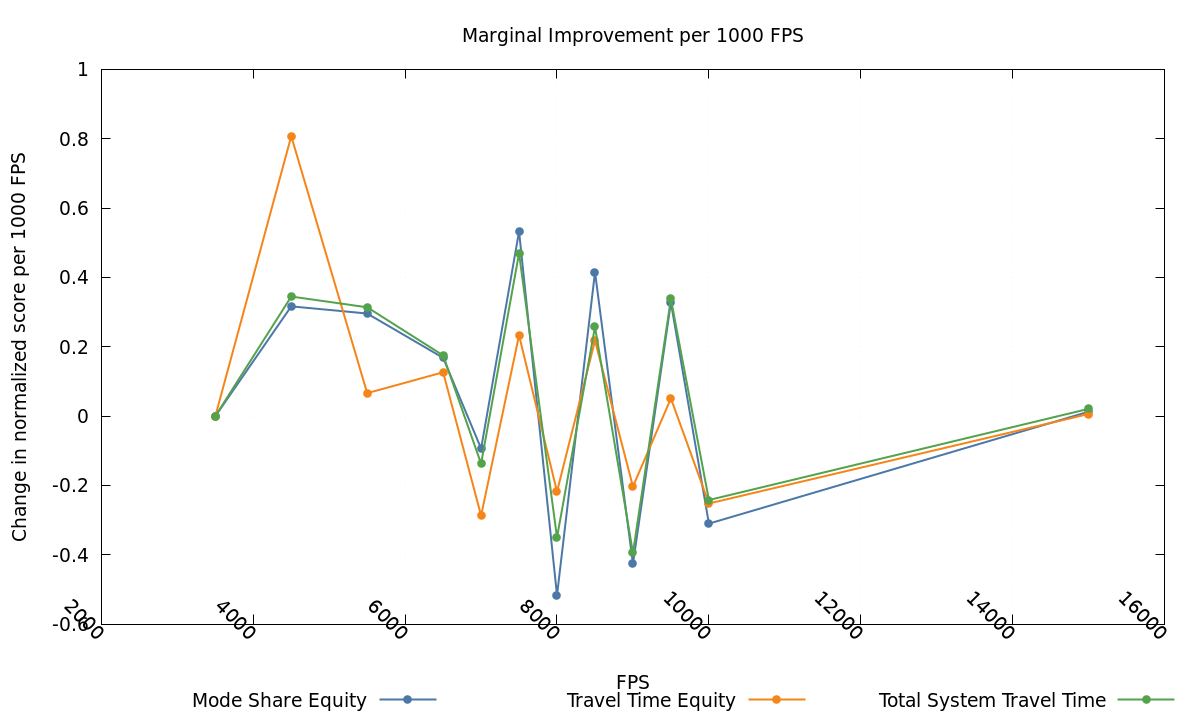
\includegraphics[width=0.8\textwidth]{cross_policy_marginal_returns.png}
\caption{Marginal-return view derived from the regenerated seed-based summaries.}
\label{fig:marginal_returns}
\end{figure}
\begin{figure}[!t]
\centering
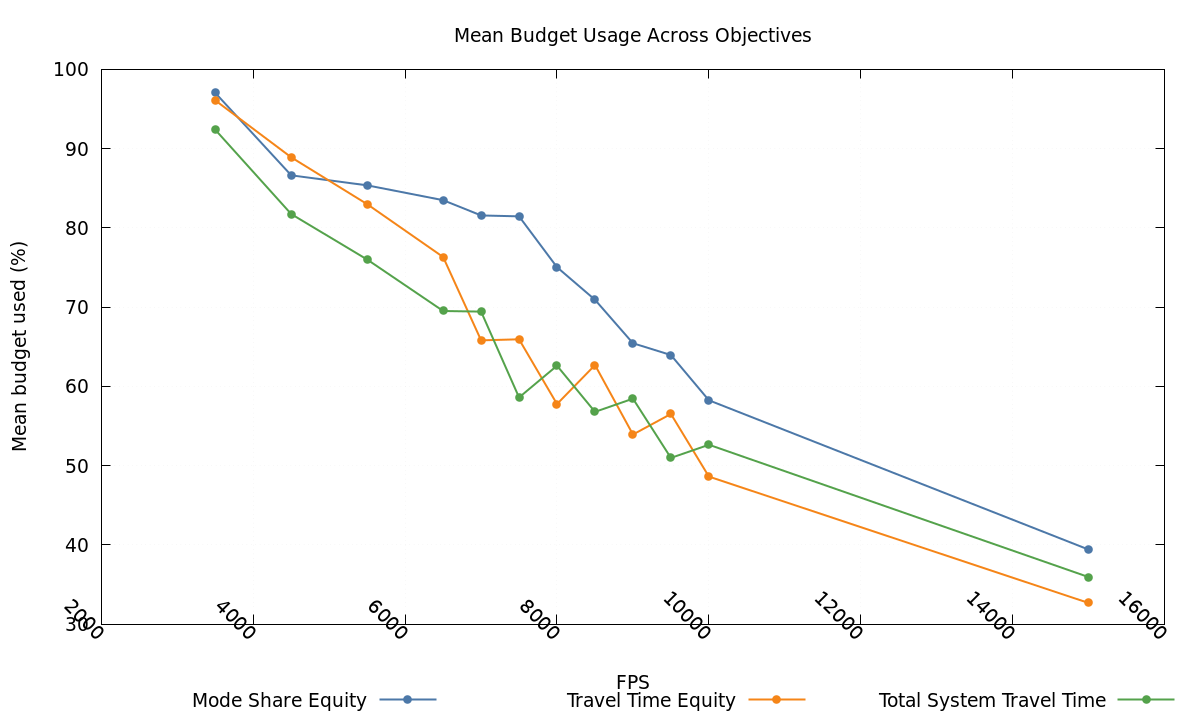
\includegraphics[width=0.8\textwidth]{cross_policy_budget_usage.png}
\caption{Budget-use curves across the three objectives using the regenerated seed-based summaries.}
\label{fig:subsidy_usage_standalone}
\end{figure}

Figures~\ref{fig:dim_returns}--\ref{fig:subsidy_usage_standalone} summarise the revised decision-support interpretation. For mode-share equity, the regenerated recommendation is FPS 7,500--9,500. For travel-time equity, it is FPS 6,500--8,500. For total system travel time, the evidence suggests a broad plateau from FPS 4,500 to 15,000, with the minimum mean at 7,500. If a single compromise value is required among the common sampled FPS points, the regenerated ranking supports FPS 7,500.

This guidance differs from the earlier manuscript in two ways. First, it is based on seed-mean performance rather than single runs. Second, it is framed as a range or plateau when the uncertainty bands and composite ranking warrant that interpretation. That is a better match to the stochastic nature of the model and to the deterministic control evidence showing saturation rather than a perfectly sharp optimum.

\section{Policy Implications and Recommendations}\label{sec:implications}

\subsection{Evidence-Based Subsidy Design Guidelines}
The revised evidence supports several narrower conclusions. In this stylised scenario, the best seed-mean FPS values cluster around 6,500--7,500 rather than 4,000--5,000. The low-income group receives the largest aggregate allocation share at each objective-specific optimum, but the observed shares are closer to 39--42\% than to the stronger progressive pattern claimed previously. Policy recommendations should therefore be framed as scenario-contingent and range-based, not as universal numerical rules. Likewise, the appearance of car-service support in some objective-specific optima should not be read as a generic recommendation to encourage car services in highly congested cities. The current scenario excludes private vehicle ownership and city-specific congestion pricing, so any car-service subsidy would need to be re-tested under local network, emissions, and policy constraints before use in practice.

\begin{table}[H]
\centering
\caption{Observed Aggregate Allocation Shares at Objective-Specific Optima}
\label{tab:progressive_structure}
\begin{tabular}{p{3.2cm}p{3cm}p{3cm}p{3cm}}
\toprule
\textbf{Objective} & \textbf{Low income} & \textbf{Middle income} & \textbf{High income} \\
\midrule
Mode Share Equity & 38.74\% & 34.91\% & 26.35\% \\
\midrule
Travel Time Equity & 41.57\% & 29.78\% & 28.65\% \\
\midrule
Total System Travel Time & 39.40\% & 32.20\% & 28.41\% \\
\bottomrule
\end{tabular}
\end{table}

\subsection{Economic Appraisal Status}\label{sec:competing-benefits}
The previous manuscript translated stylised model outputs into city-scale Australian dollar estimates and benefit-cost ratios. We do not retain those claims in the revised evidence package because the current seed-based workflow does not yet provide a reproducible mapping from abstract model units and synthetic demand to city-scale audited costs and benefits. Economic appraisal remains an important future direction, but it should be built on an empirically calibrated demand base and a verified bridge between model outputs and real-world monetary units.

\subsection{Illustrative Implementation Considerations}
The current results support only a limited implementation discussion. Any operational rollout should begin with empirical calibration, explicit eligibility design, and repeated-seed stress testing under the target city's network and demand conditions. In practical terms, city-scale transfer would require replacing the stylised grid with an empirical network, local fare and demand data, and calibrated behavioural parameters before rerunning the seed-based and deterministic checks on that case. The stylised scenario nevertheless suggests a practical workflow for pilot design and monitoring, summarised in Table \ref{tab:implementation_framework}.

\begin{table}[htbp]
\centering
\caption{Illustrative Implementation Workflow for Future Empirical Applications}
\label{tab:implementation_framework}
\begin{tabular}{p{2.5cm}p{12cm}}
\toprule
\textbf{Phase} & \textbf{Key Activities} \\
\midrule
Foundation Building: 0--6 months & 
\begin{itemize}
    \item Assemble local network, fare, and demand data
    \item Define eligibility, subsidy-delivery, and auditing rules
    \item Verify which modes and operators can receive the subsidy
    \item Reproduce the seed-based workflow on the empirical scenario
\end{itemize} \\
\midrule
Pilot Run: 6--12 months & 
\begin{itemize}
    \item Test a limited set of FPS values and allocation rules
    \item Monitor realised subsidy use, uptake heterogeneity, and spillovers
    \item Compare stochastic pilot outcomes against deterministic controls where possible
    \item Refine data and behavioural assumptions
\end{itemize} \\
\midrule
Scaled Deployment: 12--24 months & 
\begin{itemize}
    \item Expand the evaluated geography and user base
    \item Add richer behavioural and institutional constraints
    \item Re-run the optimisation and seed-based robustness analysis
    \item Audit distributional outcomes across target populations
\end{itemize} \\
\midrule
System Integration: 24+ months & 
\begin{itemize}
    \item Integrate with local MaaS, fare, and program-administration systems
    \item Add longitudinal evaluation and ex-post monitoring
    \item Extend the framework to additional objectives and policy instruments
    \item Update the evidence base as market conditions change
\end{itemize} \\
\bottomrule
\end{tabular}
\end{table}

\section{Conclusions}\label{sec:conclusions}

\subsection{Summary of Key Findings}
The revised manuscript replaces the earlier single-run narrative with a seed-based evidence package. The best seed-mean outcomes occur at FPS 7,500 for mode-share equity, FPS 6,500 for travel-time equity, and FPS 7,500 for total system travel time, with FPS 7,500 also ranking first in the regenerated cross-objective comparison among the common sampled FPS values. These results are materially different from the old 4,000--5,000 story and therefore change the paper's substantive conclusions.

The revised allocation results still direct the largest aggregate share to low-income travellers, but the effect is much weaker than previously claimed and cannot be described as a consequence of progressive bounds. In the audited optimisation scripts, all 12 allocation variables share the same 0.0--0.8 bounds. The revised manuscript therefore treats the low-income-favouring pattern as an observed property of the current experiments, not as proof of a universal progressive rule.

The deterministic fixed-policy control is central to our revised interpretation. When commuters, trip requests, and background conditions are held fixed, the FPS-response relationship becomes monotonic or near-monotonic until subsidy saturation. That supports the interpretation that the irregular objective curves in the stochastic summaries are expected consequences of ABM randomness and evolving system states, not evidence of broken optimisation logic.

\subsection{Methodological Contribution}
Methodologically, the contribution of the revision is twofold. First, it makes the workflow explicit: ABM-ETOP currently performs three separate single-objective Bayesian optimisation studies rather than a joint multi-objective optimisation. Second, it shifts the evidence base from single runs to repeated-seed summaries with uncertainty intervals and a deterministic control experiment. Together, those changes make the manuscript more reproducible and substantially more defensible.

The framework remains useful because it combines heterogeneous agents, provider responses, and a tractable optimisation loop. It can therefore expose policy plateaus, budget-saturation behaviour, and mixed allocation patterns that are hard to recover from purely aggregate models. We nevertheless present it as a stylised subsidy-allocation analysis tool, not as a fully calibrated city-scale deployment model.

\subsection{Limitations and Future Research}
The main limitations are now clearer. The study still uses a stylised grid environment, a synthetic traveller population, and a restricted set of subsidizable modes. Private vehicle ownership, private cycling, parking policy, and long-run land-use feedback are outside the present scope. These omissions matter for transferability, especially in cities where congestion, ownership, or network structure are central drivers of inequity.

The present evidence base also does not support a direct mapping from model units to city-scale costs, benefit-cost ratios, or emissions. Future work should therefore focus on empirical calibration, richer network representations, broader metric sets, and a reproducible bridge from simulation outputs to real-world appraisal. Extending the framework to joint multi-objective optimisation is also a natural next step, but it should build on the repeated-seed and deterministic-control practice established here rather than reverting to single-run comparisons.

\section{Acknowledgments}

This research was supported fully by the Australian Government through the Australian Research Council's Discovery Projects funding scheme (project DP210103138). The views expressed herein are those of the authors and are not necessarily those of the Australian Government or Australian Research Council.

\section{Declaration of Generative AI and AI-assisted Technologies in the Writing Process}

During the preparation of this work, the authors used Claude (Anthropic) in order to improve readability, language clarity, and manuscript formatting. After using this tool, the authors reviewed and edited the content as needed and take full responsibility for the content of the published article.

\bibliographystyle{cas-model2-names}
\bibliography{references}

\clearpage


\appendix
\renewcommand{\thepage}{A-\arabic{page}}
\setcounter{page}{1}


\fancypagestyle{appendixstyle}{%
  \fancyhf{}%
  \fancyfoot[C]{Page \thepage\ of \pageref{LastAppendixPage}}%
}


\pagestyle{appendixstyle}

\appendix
\section*{Appendices}
\renewcommand{\thesection}{A\arabic{section}}
\setcounter{section}{0}

\section{Agent-Based Model Development}
\label{app:abm_development}

\subsection{Model Architecture and Agent Types}
The ABM-ETOP framework employs a multi-agent architecture with three primary agent types interacting within a grid-based spatial environment. Each agent type has specific functions and behavioural characteristics:

\subsubsection{Commuter Agents}
Commuter agents represent individual transport users with heterogeneous socioeconomic attributes:
\begin{itemize}
    \item \textbf{Income group:} low, middle, or high; used in subsidy targeting, value-of-time assignment, and utility coefficients
    \item \textbf{Age:} distributed according to demographic patterns
    \item \textbf{Disability status:} boolean attribute affecting mobility constraints
    \item \textbf{Technology access:} boolean attribute affecting service usage capability
    \item \textbf{Health status:} categorized as good or poor, affecting mode preferences
    \item \textbf{Payment scheme:} PAYG or subscription, affecting pricing structure
\end{itemize}

In the current optimisation scripts, these non-income attributes are sampled independently from weighted marginals rather than from a joint demographic model. The audited weights are 0.9/0.1 for good/poor health, 0.8/0.2 for PAYG/subscription, 0.2/0.8 for disability status, and 0.95/0.05 for technology access. The sampled attributes are then used consistently in the behaviour rules: disability adds a bike/walk penalty, age $\geq 65$ or poor health adds an additional bike/walk penalty, no technology access adds a car/bike access penalty, and payment scheme affects MaaS pricing logic. We therefore treat the commuter population as a stylised implementation with explicit rule hooks, not as a fully joint empirical demographic calibration.

\subsubsection{Service Provider Agents}
Service provider agents manage transportation services with dynamic behaviours:
\begin{itemize}
    \item \textbf{Public transit:} fixed routes with time-dependent congestion patterns
    \item \textbf{Car-sharing services:} dynamic availability and pricing
    \item \textbf{Bike-sharing services:} location-based availability and dynamic pricing
    \item \textbf{Walking:} always available with fixed speed characteristics
\end{itemize}

\subsubsection{MaaS Agent}
The MaaS (Mobility-as-a-Service) agent serves as a system coordinator:
\begin{itemize}
    \item \textbf{Trip request processing:} matches commuter needs with available options
    \item \textbf{Route optimisation:} generates efficient multi-modal routes
    \item \textbf{Subsidy application:} implements subsidy policies across modes
    \item \textbf{Service booking:} facilitates transactions between commuters and providers
    \item \textbf{Congestion modeling:} captures traffic dynamics across the network
\end{itemize}


\subsection{Definitive Parameter Reference Table}
\label{app:definitive_params}

\begin{table}[!ht]
\centering
\caption{Definitive Model Parameters (Single Source of Truth)}
\small
\begin{tabularx}{\textwidth}{p{0.22\textwidth}p{0.16\textwidth}p{0.14\textwidth}Y}
\toprule
\textbf{Parameter} & \textbf{Value} & \textbf{Unit} & \textbf{Notes} \\
\midrule
\multicolumn{4}{l}{\textbf{Scenario Size}} \\
Commuters & 200 & agents & Current optimisation scripts \\
Grid width & 100 & cells & Current optimisation scripts \\
Grid height & 100 & cells & Current optimisation scripts \\
Simulation horizon & 144 & time steps & Within-run resolution, not BO iterations \\
\midrule
\multicolumn{4}{l}{\textbf{Utility and Time Values}} \\
$\beta_C$ (Cost) & -0.15 & - & Base value \\
$\beta_T$ (Time) & -0.09 & - & Base value \\
$\beta_W$ (Modal) & -0.04 & - & Modal penalty \\
$\beta_A$ (Affordability) & -0.04 & - & Affordability adjustment \\
High-income car $\beta_C$ & -0.02 & - & Lower price sensitivity for the special car term \\
Low VOT & 5.00 & \$/hour & Before flexibility adjustment \\
Middle VOT & 10.00 & \$/hour & Before flexibility adjustment \\
High VOT & 20.00 & \$/hour & Before flexibility adjustment \\
\midrule
\multicolumn{4}{l}{\textbf{Congestion and Demand}} \\
Background traffic & 200 & vehicles & Exogenous background traffic amount \\
$\alpha$ & 0.03 & - & BPR congestion parameter \\
$\beta$ & 1.5 & - & BPR congestion parameter \\
Income weights & [0.5, 0.3, 0.2] & share & Low, middle, high commuter shares \\
Health weights & [0.9, 0.1] & share & Good, poor \\
Payment weights & [0.8, 0.2] & share & PAYG, subscription \\
Disability weights & [0.2, 0.8] & share & True, false \\
Technology-access weights & [0.95, 0.05] & share & True, false \\
\midrule
\multicolumn{4}{l}{\textbf{Optimisation Controls}} \\
Allocation bounds & 0.0--0.8 & proportion & Applied uniformly to all 12 decision variables \\
Initial BO samples & 8 & matrices & Latin-hypercube initial design \\
BO updates (mode share) & 10 & iterations/FPS & Current script setting \\
BO updates (time, TSTT) & 3 & iterations/FPS & Current script setting \\
Recovered job requests & 15--16 CPUs; 32--124 GB; 11--12 h walltime & PBS request & Requested resources in preserved Katana job scripts, not measured runtimes \\
\bottomrule
\end{tabularx}
\end{table}

\subsection{Commuter Decision-Making Process}
\subsubsection{Utility Function Formulation}
The core decision-making mechanism for commuter agents is based on a random utility maximisation framework. For each available transportation option, the utility is calculated as:

\begin{equation}
U_{i,j} = \text{ASC}_j + \beta_C \cdot (C_{i,j} - S_{i,j}) + \beta_T \cdot \text{VOT}_i \cdot T_{i,j} + \beta_W \cdot W_{i,j} + \beta_A \cdot A_{i,j}
\end{equation}

Where:
\begin{itemize}
    \item $U_{i,j}$: Utility of mode $j$ for commuter from income group $i$
    \item $\text{ASC}_j$: Alternative-specific constant for mode $j$
    \item $\beta_C$: Cost sensitivity coefficient (negative value)
    \item $C_{i,j}$: Original cost of mode $j$ for income group $i$
    \item $S_{i,j}$: Subsidy amount for mode $j$ and income group $i$
    \item $\beta_T$: Time sensitivity coefficient (negative value)
    \item $\text{VOT}_i$: Value of time for income group $i$
    \item $T_{i,j}$: Travel time for mode $j$
    \item $\beta_W$: Modal penalty coefficient
    \item $W_{i,j}$: Modal penalty for mode $j$ (e.g., disability accessibility)
    \item $\beta_A$: Affordability coefficient
    \item $A_{i,j}$: Affordability adjustment for mode $j$
\end{itemize}

\subsubsection{Modal Choice Probability}
The probability of selecting each transportation mode is calculated using the multinomial logit model:

\begin{equation}
P(j|i) = \frac{\exp(U_{i,j})}{\sum_{k \in M} \exp(U_{i,k})}
\end{equation}

Where:
\begin{itemize}
    \item $P(j|i)$: Probability of commuter from income group $i$ choosing mode $j$
    \item $M$: Set of all available modes
\end{itemize}

\subsubsection{Value of Time Calculation}
The value of time (VOT) is income-dependent and adjusted by trip purpose flexibility:

\begin{equation}
\text{VOT}_i = \text{VOT}_{\text{base},i} \cdot f_{\text{flexibility}}
\end{equation}

Where:
\begin{itemize}
    \item $\text{VOT}_{\text{base},i}$: Base value of time for income group $i$
    \item $f_{\text{flexibility}}$: Adjustment factor based on trip purpose flexibility
\end{itemize}

The base values of time used in the model are:
\begin{itemize}
    \item Low income: \$5 per hour 
    \item Middle income: \$10 per hour 
    \item High income: \$20 per hour 
\end{itemize}

The flexibility adjustment factors vary by trip purpose:
\begin{itemize}
    \item Low flexibility (work, school, medical): 1.15
    \item Medium flexibility (default): 1.00
    \item High flexibility (shopping, leisure): 0.85
\end{itemize}

\subsubsection{Trip Generation Algorithm}
Commuter agents generate trip requests based on their socioeconomic characteristics and temporal patterns, implemented as follows:

\begin{algorithm}
\caption{Stochastic Trip Generation with Socioeconomic Stratification}
\label{alg:trip-generation}
\begin{algorithmic}[1]
\Require Commuter agent $c$, current time $t$, demographic parameters $\Theta_c$
\Ensure Trip request $r$ or $\emptyset$
\State $P_{base} \gets$ ComputeBaseProbability($\Theta_c$.income, $\Theta_c$.age, $\Theta_c$.disability)
\State $\mu_{temporal} \gets$ TemporalMultiplier($t$, WeekdayStatus($t$))
\If{WeekdayStatus($t$) = weekend}
    \State $\mu_{temporal} \gets \mu_{temporal} \times$ GaussianKernel($t_{midday}$, $\sigma_{weekend}$)
\Else
    \State $\mu_{temporal} \gets \max($GaussianKernel($t_{morning}$, $\sigma_{peak}$), GaussianKernel($t_{evening}$, $\sigma_{peak}$), $\epsilon_{base})$
\EndIf
\State $P_{trip} \gets P_{base} \times \mu_{temporal} \times$ PaymentSchemeMultiplier($\Theta_c$.payment)
\If{$\text{uniform}(0,1) < P_{trip}$ and $\neg$HasActiveRequest($c$)}
    \State $\tau_{purpose} \gets$ SelectTravelPurpose($t$, $\Theta_c$)
    \State $d \gets$ GenerateDestination($\tau_{purpose}$, $c$.location, $\Theta_c$)
    \State $t_{start} \gets t + \text{uniform}(\Delta t_{min}, \Delta t_{max})$
    \State $r \gets$ CreateRequest(GenerateUUID(), $c$.location, $d$, $t_{start}$, $\tau_{purpose}$)
    \State \Return $r$
\EndIf
\State \Return $\emptyset$
\end{algorithmic}
\end{algorithm}

The function $\texttt{calculateTimeMultiplier}(t)$ models temporal patterns by applying a non-uniform distribution across the day:

\begin{equation}
\texttt{time\_multiplier} = 
\begin{cases}
3.0 \cdot \exp\left(-0.5 \cdot \left(\frac{t_{\text{day}} - 48}{8}\right)^2\right) & \text{for morning peak} \\
2.5 \cdot \exp\left(-0.5 \cdot \left(\frac{t_{\text{day}} - 105}{10}\right)^2\right) & \text{for evening peak} \\
\max(\text{morning\_intensity}, \text{evening\_intensity}, 0.2) & \text{for weekdays} \\
1.5 \cdot \exp\left(-0.5 \cdot \left(\frac{t_{\text{day}} - 72}{16}\right)^2\right) & \text{for weekends}
\end{cases}
\end{equation}

Where $t_{\text{day}}$ is the time of day (modulo 144 ticks, with each tick representing 10 minutes).

\subsection{MaaS Agent Algorithms}
\subsubsection{Congestion Modeling}

The MaaS agent employs the Bureau of Public Roads (BPR) function to model congestion effects on travel times:

\begin{equation}
T_{ij} = T_{ij\_\text{free\_flow}} \times \left(1 + \alpha \times \left(\frac{V_{ij}}{C_{ij}}\right)^{\beta}\right)
\end{equation}

Where:
\begin{itemize}
    \item $T_{ij}$: Congested travel time between points $i$ and $j$
    \item $T_{ij\_\text{free\_flow}}$: Free-flow travel time between points $i$ and $j$
    \item $\alpha$: Congestion parameter (0.03 in the model)
    \item $\beta$: Congestion parameter (1.5 in the model)
    \item $V_{ij}$: Traffic volume between points $i$ and $j$
    \item $C_{ij}$: Capacity between points $i$ and $j$
\end{itemize}

\subsubsection{Traffic Volume Calculation}
The MaaS agent determines the current traffic volume by aggregating all active bookings affecting a particular network segment:

\begin{algorithm}
\caption{Dynamic Traffic Volume Aggregation}
\label{alg:traffic-aggregation}
\begin{algorithmic}[1]
\Require Current time step $t$, active booking set $\mathcal{B}$
\Ensure Traffic volume mapping $\mathcal{V}: E \rightarrow \mathbb{N}$
\State $\mathcal{V} \gets \{\}$, $\mathcal{S}_{processed} \gets \emptyset$
\For{$b \in \mathcal{B}$ where $t \in b$.AffectedSteps}
    \State $\rho \gets b$.RouteDetails
    \For{$i \gets 0$ to $|\rho| - 2$}
        \State $e \gets (\rho[i], \rho[i+1])$, $e_{rev} \gets (\rho[i+1], \rho[i])$
        \If{$e \notin \mathcal{S}_{processed}$}
            \State $\mathcal{S}_{processed} \gets \mathcal{S}_{processed} \cup \{e, e_{rev}\}$
            \State $\mathcal{V}[e] \gets \mathcal{V}[e] + 1$
            \State $\mathcal{V}[e_{rev}] \gets \mathcal{V}[e_{rev}] + 1$
        \EndIf
    \EndFor
\EndFor
\State \Return $\mathcal{V}$
\end{algorithmic}
\end{algorithm}

\subsubsection{Modified Dijkstra's Algorithm with Congestion}
The MaaS agent uses a modified Dijkstra's algorithm to find shortest paths while accounting for congestion:

\begin{algorithm}
\caption{Congestion-Aware Shortest Path Algorithm}
\label{alg:congestion-dijkstra}
\begin{algorithmic}[1]
\Require Graph $G = (V, E)$, source $s$, target $e$, mode $m$, traffic state $\mathcal{V}$
\Ensure Shortest path $\pi^*$ or fallback path
\State $d \gets$ InitializeDistances($V$, $s$), $\pi \gets \{\}$
\State $Q \gets$ PriorityQueue(), $Q$.insert($(0, s)$)
\State $\mathcal{V}_{traffic} \gets$ GetTrafficVolume($t$)
\While{$Q \neq \emptyset$}
    \State $(d_{curr}, v_{curr}) \gets Q$.extractMin()
    \If{$v_{curr} = e$}
        \State \textbf{break}
    \EndIf
    \For{$v_{next} \in$ Neighbors($v_{curr}$)}
        \State $w_{edge} \gets$ ComputeEdgeWeight($v_{curr}$, $v_{next}$, $m$, $\mathcal{V}_{traffic}$)
        \If{$m =$ CAR\_MODE}
            \State $w_{edge} \gets w_{free} \times \text{BPR}(\mathcal{V}_{traffic}[(v_{curr}, v_{next})], C_{edge})$
        \EndIf
        \If{$d_{curr} + w_{edge} < d[v_{next}]$}
            \State $d[v_{next}] \gets d_{curr} + w_{edge}$
            \State $\pi[v_{next}] \gets v_{curr}$
            \State $Q$.insert($(d[v_{next}], v_{next})$)
        \EndIf
    \EndFor
\EndWhile
\State \Return ReconstructPath($\pi$, $s$, $e$) $\lor$ ManhattanFallback($s$, $e$)
\end{algorithmic}
\end{algorithm}

\subsubsection{Multi-Modal Route Generation}
For public transportation and MaaS options, the algorithm consists of two phases: finding the optimal sequence of public transport services, and building a detailed itinerary with access/egress modes:

\begin{algorithm}
\caption{Multi-Modal Public Transport Route Discovery}
\label{alg:multimodal-routing}
\begin{algorithmic}[1]
\Require Origin $o$, destination $d$, station network $\mathcal{S}$, route network $\mathcal{R}$, transfer network $\mathcal{T}$
\Ensure Optimal station sequence $\sigma^*$ or $\emptyset$
\State $(m_o, s_o) \gets$ FindNearestStation($o$, $\mathcal{S}$)
\State $(m_d, s_d) \gets$ FindNearestStation($d$, $\mathcal{S}$)
\State $\tau \gets$ InitializeArrivalTimes($\mathcal{S}$), $\tau[s_o] \gets 0$
\State $\Pi \gets \{\}$, $Q \gets$ PriorityQueue()
\State $Q$.insert($(0, s_o)$)
\While{$Q \neq \emptyset$ and $Q$.top().station $\neq s_d$}
    \State $(t_{curr}, s_{curr}) \gets Q$.extractMin()
    \For{$m \in \{\text{BUS}, \text{TRAIN}\}$}
        \For{$r \in$ GetRoutesThrough($m$, $s_{curr}$)}
            \State $\sigma_r \gets \mathcal{R}[m][r]$
            \State $idx \gets$ IndexOf($s_{curr}$, $\sigma_r$)
            \For{$s_{next} \in$ AdjacentStations($\sigma_r$, $idx$)}
                \State $t_{arr} \gets t_{curr} + \text{STOP\_TIME}$
                \If{$t_{arr} < \tau[s_{next}]$}
                    \State $\tau[s_{next}] \gets t_{arr}$, $\Pi[s_{next}] \gets s_{curr}$
                    \State $Q$.insert($(t_{arr}, s_{next})$)
                \EndIf
            \EndFor
        \EndFor
    \EndFor
    \For{$(s_{transfer}, t_{transfer}) \in \mathcal{T}[s_{curr}]$}
        \State $t_{arr} \gets t_{curr} + t_{transfer}$
        \If{$t_{arr} < \tau[s_{transfer}]$}
            \State $\tau[s_{transfer}] \gets t_{arr}$, $\Pi[s_{transfer}] \gets s_{curr}$
            \State $Q$.insert($(t_{arr}, s_{transfer})$)
        \EndIf
    \EndFor
\EndWhile
\State \Return ReconstructPath($\Pi$, $s_o$, $s_d$)
\end{algorithmic}
\end{algorithm}

\begin{algorithm}
\caption{Round-Based Public Transit Optimized Router (RAPTOR)}
\label{alg:raptor}
\begin{algorithmic}[1]
\Require Origin $o$, destination $d$, departure time $\tau_0$, route network $\mathcal{R}$, stop network $\mathcal{S}$
\Ensure Pareto-optimal journey set $\mathcal{J}^*$
\State $\tau^{(0)} \gets$ InitializeArrivalTimes($\mathcal{S}$, $\infty$)
\State $\tau^{(0)}[$ NearestStop($o$)$] \gets \tau_0$
\State $\mathcal{J}^* \gets \emptyset$, $k \gets 0$
\Repeat
    \State $k \gets k + 1$
    \State $\tau^{(k)} \gets \tau^{(k-1)}$ \Comment{Initialize round $k$}
    \State $\mathcal{Q} \gets \emptyset$ \Comment{Queue of marked stops}
    \Comment{Accumulate routes serving marked stops}
    \For{$s \in \mathcal{S}$ where $\tau^{(k-1)}[s] < \tau^{(k-2)}[s]$}
        \For{$r \in$ RoutesServing($s$)}
            \State $\mathcal{Q} \gets \mathcal{Q} \cup \{r\}$
        \EndFor
    \EndFor
    \Comment{Traverse each marked route}
    \For{$r \in \mathcal{Q}$}
        \State $t_{board} \gets \infty$, $s_{board} \gets \emptyset$
        \For{$s \in$ StopsOf($r$) in route order}
            \If{$\tau^{(k-1)}[s] < t_{board}$}
                \State $t_{board} \gets \tau^{(k-1)}[s]$, $s_{board} \gets s$
            \EndIf
            \If{$s_{board} \neq \emptyset$ and CanReach($s_{board}$, $s$, $r$)}
                \State $t_{arr} \gets t_{board} +$ TravelTime($s_{board}$, $s$, $r$)
                \If{$t_{arr} < \tau^{(k)}[s]$}
                    \State $\tau^{(k)}[s] \gets t_{arr}$
                \EndIf
            \EndIf
        \EndFor
    \EndFor
    \Comment{Handle footpath transfers}
    \For{$s \in \mathcal{S}$ where $\tau^{(k)}[s] < \tau^{(k-1)}[s]$}
        \For{$s' \in$ FootpathReachable($s$)}
            \State $t_{arr} \gets \tau^{(k)}[s] +$ WalkTime($s$, $s'$)
            \State $\tau^{(k)}[s'] \gets \min(\tau^{(k)}[s'], t_{arr})$
        \EndFor
    \EndFor
    \Comment{Update destination arrivals}
    \State $s_d \gets$ NearestStop($d$)
    \If{$\tau^{(k)}[s_d] < \infty$}
        \State $\mathcal{J}^* \gets \mathcal{J}^* \cup \{(\tau^{(k)}[s_d], k)\}$
    \EndIf
\Until{$\tau^{(k)} = \tau^{(k-1)}$ or $k > k_{max}$}
\State \Return ExtractParetoOptimal($\mathcal{J}^*$)
\end{algorithmic}
\end{algorithm}

\subsection{Service Provider Agent Algorithms}
\subsubsection{Dynamic Pricing Algorithm}
The service provider agent applies dynamic pricing based on demand-to-capacity ratios:

\begin{equation}
P_{\text{dynamic}} = P_{\text{base}} \cdot \left(1 + \alpha \cdot (DRC - DRC_{\text{base}}) \cdot (1 + \text{Demand}_{\text{change}})\right)
\end{equation}

Where:
\begin{itemize}
    \item $P_{\text{dynamic}}$: Adjusted dynamic price
    \item $P_{\text{base}}$: Base price for the service
    \item $\alpha$: Provider-specific sensitivity coefficient (0.25-0.5)
    \item $DRC$: Current demand-to-capacity ratio
    \item $DRC_{\text{base}}$: Baseline demand-to-capacity ratio (typically 0.5)
    \item $\text{Demand}_{\text{change}}$: Rate of change in demand
\end{itemize}

\begin{algorithm}
\caption{Demand-Responsive Dynamic Pricing}
\label{alg:dynamic-pricing}
\begin{algorithmic}[1]
\Require Service provider set $\mathcal{P}$, current step $t$, demand history $\mathcal{H}$
\Ensure Updated pricing matrix $\mathbf{P}^{(t+1)}$
\For{$p \in \mathcal{P}$}
    \State $\alpha_p \gets$ GetSensitivityCoefficient($p$)
    \State $\rho_{baseline} \gets 0.5$ \Comment{Baseline demand-capacity ratio}
    \For{$\Delta t \in \{0, 1, 2, 3, 4, 5\}$} \Comment{Future time slots}
        \State $\text{cap}_p \gets$ GetCapacity($p$)
        \State $\text{avail}_{p,\Delta t} \gets$ GetAvailability($p$, $t + \Delta t$)
        \State $\text{occ}_{p,\Delta t} \gets \text{cap}_p - \text{avail}_{p,\Delta t}$
        \State $\rho_{p,\Delta t} \gets \text{occ}_{p,\Delta t} / \text{cap}_p$
        \State $\Delta\rho_p \gets$ ComputeDemandChange($\mathcal{H}$, $p$, $\Delta t$)
        \If{$\rho_{p,\Delta t} < \rho_{baseline}$}
            \State $\mu_{price} \gets -\alpha_p \times (\rho_{baseline} - \rho_{p,\Delta t}) \times (1 + \Delta\rho_p)$
        \Else
            \State $\mu_{price} \gets \alpha_p \times (\rho_{p,\Delta t} - \rho_{baseline}) \times (1 + \Delta\rho_p)$
        \EndIf
        \State $P_{p,\Delta t}^{(t+1)} \gets P_{p,\Delta t}^{(t)} \times (1 + \mu_{price})$
        \State $P_{p,\Delta t}^{(t+1)} \gets$ Clamp($P_{p,\Delta t}^{(t+1)}$, $0.2 \times P_{base}$, $1.8 \times P_{base}$)
    \EndFor
\EndFor
\State \Return $\mathbf{P}^{(t+1)}$
\end{algorithmic}
\end{algorithm}

\subsubsection{Service Availability Tracking}
Service providers track availability by continually updating bookings and capacity:

\begin{algorithm}
\caption{Update Service Availability}
\begin{algorithmic}[1]
\State \textbf{Input:} Current step $t$
\State \textbf{Output:} Updated availability for all services
\State $\texttt{service\_tables} \gets [\texttt{UberLike1}, \texttt{UberLike2}, \texttt{BikeShare1}, \texttt{BikeShare2}]$
\State $\texttt{booking\_logs} \gets \texttt{query\_all\_booking\_logs}()$
\For{$\texttt{service\_table\_name}$ in $\texttt{service\_tables}$}
    \State $\texttt{service\_table} \gets \texttt{get\_service\_table}(\texttt{service\_table\_name})$
    \State $\texttt{new\_services} \gets \texttt{query}(\texttt{service\_table}, \texttt{step\_count} \geq t)$
    \For{$\texttt{new\_service}$ in $\texttt{new\_services}$}
        \State $\texttt{step\_offset} \gets \texttt{new\_service.step\_count} - t$
        \If{$\texttt{step\_offset} < 6$} \Comment{Only interested in next 6 steps}
            \State $\texttt{availability\_updates} \gets [\texttt{get}(\texttt{new\_service}, \texttt{availability\_} + i, \texttt{new\_service.capacity}) \text{ for } i \in \{0, 1, 2, 3, 4, 5\}]$
            \For{$\texttt{booking}$ in $\texttt{booking\_logs}$}
                \If{$\texttt{booking.company\_name} = \texttt{new\_service.company\_name}$}
                    \For{$\texttt{step}$ in $\{0, 1, 2, 3, 4, 5\}$}
                        \State $\texttt{step\_count} \gets t + \texttt{step}$
                        \If{$\texttt{step\_count} \in \texttt{booking.affected\_steps}$}
                            \State $\texttt{availability\_updates}[\texttt{step}] \gets \texttt{availability\_updates}[\texttt{step}] - 1$
                        \EndIf
                    \EndFor
                \EndIf
            \EndFor
            \For{$i \gets 0$ to $5$}
                \If{$\texttt{step\_offset} + i < 6$}
                    \State $\texttt{set}(\texttt{new\_service}, \texttt{availability\_} + (\texttt{step\_offset} + i), \texttt{availability\_updates}[\texttt{step\_offset} + i])$
                \EndIf
            \EndFor
        \EndIf
    \EndFor
\EndFor
\end{algorithmic}
\end{algorithm}

\subsection{Subsidy Pool Mechanism}
The ABM-ETOP framework implements a Fixed Pool Subsidy (FPS) mechanism with various pool types (daily, weekly, monthly). The core algorithm for checking subsidy availability is:

\begin{algorithm}
\caption{Fixed Pool Subsidy Allocation}
\label{alg:subsidy-allocation}
\begin{algorithmic}[1]
\Require Requested amount $r$, current time $t$, pool configuration $\mathcal{C}$, usage log $\mathcal{L}$
\Ensure Granted subsidy amount $s \leq r$
\State $t_{day} \gets \lfloor t / \text{TICKS\_PER\_DAY} \rfloor$
\State $t_{week} \gets \lfloor t_{day} / 7 \rfloor$
\State $\text{dow} \gets t_{day} \bmod 7$
\If{$\text{dow} \geq 5$} \Comment{Weekend check}
    \State \Return $0$
\EndIf
\If{$\mathcal{C}$.pool\_type = WEEKLY}
    \State $U_{total} \gets \sum_{l \in \mathcal{L}} l$.amount where $l$.week $= t_{week}$
\ElsIf{$\mathcal{C}$.pool\_type = DAILY}
    \State $U_{total} \gets \sum_{l \in \mathcal{L}} l$.amount where $l$.day $= t_{day}$
\ElsIf{$\mathcal{C}$.pool\_type = MONTHLY}
    \State $U_{total} \gets \sum_{l \in \mathcal{L}} l$.amount where $l$.month $= \lfloor t_{day} / 30 \rfloor$
\EndIf
\State $R_{pool} \gets \mathcal{C}$.total\_amount $- U_{total}$
\If{$R_{pool} \geq r$}
    \State \Return $r$ \Comment{Full subsidy granted}
\ElsIf{$R_{pool} > 0$}
    \State \Return $R_{pool}$ \Comment{Partial subsidy granted}
\Else
    \State \Return $0$ \Comment{Pool depleted}
\EndIf
\end{algorithmic}
\end{algorithm}

The Fixed Pool Subsidy is implemented with a reset mechanism based on the selected pool type:

\begin{equation}
\text{is\_reset\_time}(t, \text{last\_reset}) = 
\begin{cases}
\text{current\_day} > \text{last\_reset\_day} & \text{if pool\_type = daily} \\
\text{current\_week} > \text{last\_week} \text{ and day\_of\_week = 0} & \text{if pool\_type = weekly} \\
\text{current\_month} > \text{last\_month} & \text{if pool\_type = monthly}
\end{cases}
\end{equation}

\section{Parameter Specifications}
\label{app:param_specs}

This appendix section records the current audited parameter structure used by the revised manuscript. The vectors $\mathbf{S}$, $\mathbf{P}$, $\mathbf{A}$, and $\mathbf{E}$ are interpreted as implementation groupings rather than as claims that every element is externally calibrated.

\subsection{System Parameters \texorpdfstring{($\mathbf{S}$)}{(S)}}
The system vector $\mathbf{S}$ contains the behavioural and network parameters that remain fixed during a simulation run:

\begin{equation}
\mathbf{S} = \begin{bmatrix} \boldsymbol{\beta} \\ \text{ASC} \\ \text{VOT} \\ \mathbf{N} \end{bmatrix}
\end{equation}

In the current scripts, the base utility coefficients are $\beta_C=-0.15$, $\beta_T=-0.09$, $\beta_W=-0.04$, and $\beta_A=-0.04$, with a special high-income car coefficient $\beta_C=-0.02$. The base values of time are \$5, \$10, and \$20 per hour for low-, middle-, and high-income travellers, respectively. The congestion parameters are $\alpha=0.03$ and $\beta=1.5$, and the background traffic amount is 200. These values were audited directly from the three optimisation scripts used in the revision.

\subsection{Policy Parameters \texorpdfstring{($\mathbf{P}$)}{(P)}}
The policy vector groups the exogenous subsidy controls:

\begin{equation}
\mathbf{P} = \begin{bmatrix} \text{FPS} \\ \mathbf{A}_{\text{alloc}} \end{bmatrix}
\end{equation}

Here, FPS denotes the fixed-pool subsidy budget and $\mathbf{A}_{\text{alloc}}$ denotes the 12-cell subsidy-allocation matrix across income groups and mode classes. In the revised workflow, the sampled FPS set contains 12 values: 3,500, 4,500, 5,500, 6,500, 7,000, 7,500, 8,000, 8,500, 9,000, 9,500, 10,000, and 15,000. All 12 allocation variables share the same box constraints, $0.0 \leq a_{i,m} \leq 0.8$.

\subsection{Agent Parameters \texorpdfstring{($\mathbf{A}$)}{(A)}}
The agent vector collects the state variables and behavioural rules of commuters, service providers, and the system coordinator:

\begin{equation}
\mathbf{A} = \begin{bmatrix} \mathbf{C} \\ \mathbf{SP} \\ \mathbf{SC} \end{bmatrix}
\end{equation}

\begin{itemize}
    \item $\mathbf{C}$ contains commuter attributes such as income group, age, disability status, health status, payment scheme, and technology access. The current commuter income weights are $[0.5, 0.3, 0.2]$ for low, middle, and high income.
    \item $\mathbf{SP}$ contains service-provider operating rules including capacities, dynamic pricing parameters, and mode-specific fares.
    \item $\mathbf{SC}$ contains system-coordinator logic such as routing, booking, and subsidy-application rules.
\end{itemize}

\subsection{Environment Parameters \texorpdfstring{($\mathbf{E}$)}{(E)}}
The environment vector contains exogenous setting variables:

\begin{equation}
\mathbf{E} = \begin{bmatrix} \mathbf{G} \\ \mathbf{T} \end{bmatrix}
\end{equation}

In the revised scripts, $\mathbf{G}$ contains the 100$\times$100 grid geometry and associated infrastructure placement, while $\mathbf{T}$ contains the 144-step daily time resolution and peak-period structure. Realised trip requests are not part of $\mathbf{E}$; they are endogenous outcomes generated by commuter agents within that environment.

\section{Optimisation Methodology}
\label{app:optimization}

\subsection{Bayesian Optimization with Gaussian Process Regression}
The revised manuscript is based on three separate single-objective Bayesian optimisation runs, not on a single multi-objective optimiser. The optimisation problem can be written as:

\begin{equation}
\mathbf{A}^* = \underset{\mathbf{A}}{\text{argmin}} \, M(\mathbf{A})
\end{equation}

where $M(\mathbf{A})$ is one of $E_{\text{mode}}$, $E_{\text{time}}$, or $T_{\text{total}}$.

\subsection{Parameter Space and Constraints}
Each optimisation uses the same 12-dimensional decision space: 3 income groups multiplied by 4 mode classes. The revised scripts generate 8 Latin-hypercube initial samples and then perform Bayesian updates. The mode-share script uses 10 updates per FPS value; the travel-time-equity and total-system-travel-time scripts use 3 updates per FPS value. The common parameter bounds are shown in Table~\ref{tab:appendix_bounds}.

Across the 12 sampled FPS values, this implies 216 Bayesian-optimisation objective evaluations for mode-share equity and 132 each for travel-time equity and total system travel time before the retained-policy seed checks. The repeated-seed stage then adds 360 retained-policy runs per objective because each sampled FPS value is re-evaluated over 30 stochastic seeds.

\begin{table}[!h]
\centering
\caption{Uniform Subsidy Allocation Bounds in the Revised Optimisation Scripts}
\label{tab:appendix_bounds}
\begin{tabular}{lccc}
\toprule
\textbf{Income Level} & \textbf{Mode Class} & \textbf{Lower Bound} & \textbf{Upper Bound} \\
\midrule
Low & Bike, Car, MaaS Bundle, Public & 0.0 & 0.8 \\
Middle & Bike, Car, MaaS Bundle, Public & 0.0 & 0.8 \\
High & Bike, Car, MaaS Bundle, Public & 0.0 & 0.8 \\
\bottomrule
\end{tabular}
\end{table}

The key clarification for this revision is that the 144 simulation steps are within-run time steps, not optimisation iterations. Stochasticity is handled after optimisation by re-running the retained policy for each sampled FPS value over 30 seeds and then aggregating the outcomes.

The preserved execution scripts also document the compute environment more precisely than the prior draft did. The main mode-share optimisation PBS script requests 1 node with 15 CPUs, 32 GB memory, and 12 hours walltime, while the seed-array evaluation PBS script requests 1 node with 16 CPUs, 124 GB memory, and 11 hours walltime. Preserved scheduler outputs also provide measured runtimes for part of the workflow: the travel-time and total-system one-FPS deterministic jobs each completed in about 1 hour 48 minutes, the fixed-policy deterministic sweeps completed in about 1 hour 50 minutes to 2 hours 14 minutes, and preserved total-system seed-array jobs completed in about 6 hours 34 minutes to 9 hours 16 minutes on 10 CPUs. We still do not have equally complete measured walltimes for every optimisation objective in the revised package.

\subsection{Policy Objectives and Metrics}
\label{subsec:policy_objectives}
The three reported objectives remain:

\begin{itemize}
    \item \textbf{Mode-share equity} $E_{\text{mode}}$: dimensionless, because the code applies a scaling function to weighted mode-share deviations.
    \item \textbf{Travel-time equity} $E_{\text{time}}$: reported in minutes because it sums absolute deviations of income-group mean travel times from the overall mean.
    \item \textbf{Total system travel time} $T_{\text{total}}$: reported in minutes as the aggregate travel time over all trips.
\end{itemize}

Because these metrics have different units and interpretations, the manuscript does not treat them as directly comparable on a common raw scale. Any cross-objective comparison is explicitly normalised for decision-support purposes.

\section{Calibration and Validation}
\label{app:calibration_validation}

\subsection{Current Status of Calibration}
The revised appendix distinguishes between implemented parameters and externally validated parameters. The key values used in the manuscript were audited directly from the optimisation scripts. This establishes reproducibility of the implementation, but it does not yet constitute full empirical calibration to a specific city. In particular, the stylised grid geometry, synthetic population, independently sampled commuter attributes, and behavioural simplifications mean that the results should be interpreted as scenario-analysis evidence rather than as a calibrated forecast.

\begin{table}[!ht]
\centering
\caption{Implementation Parameters Audited Directly from the Revised Optimisation Scripts}
\small
\begin{tabularx}{\textwidth}{p{0.24\textwidth}p{0.32\textwidth}Y}
\toprule
\textbf{Parameter Group} & \textbf{Current Value(s)} & \textbf{Source in Revision Workflow} \\
\midrule
Scenario size & 200 commuters; 100$\times$100 grid; 144 steps & Three optimisation scripts \\
Income weights & [0.5, 0.3, 0.2] & Three optimisation scripts \\
Base utility coefficients & $\beta_C=-0.15$, $\beta_T=-0.09$, $\beta_W=-0.04$, $\beta_A=-0.04$ & Three optimisation scripts \\
Special high-income car term & $\beta_C=-0.02$, $\beta_T=-0.09$ & Three optimisation scripts \\
Value of time & low 5, middle 10, high 20 & Three optimisation scripts \\
Congestion settings & background traffic 200; $\alpha=0.03$; $\beta=1.5$ & Three optimisation scripts \\
Commuter attribute weights & health [0.9, 0.1]; payment [0.8, 0.2]; disability [0.2, 0.8]; tech access [0.95, 0.05] & Three optimisation scripts \\
\bottomrule
\end{tabularx}
\end{table}

These audited values should be read as implementation settings for the stylised scenario unless a separate empirical source is cited in the main text or bibliography. In other words, the current appendix resolves the script-level provenance of the parameters, but it does not claim that every behavioural constant has already been calibrated to an external benchmark dataset.

\subsection{Validation and Internal Checks}
The current revision does not claim external statistical validation against a city-scale benchmark. Instead, it relies on three internal checks:

\begin{itemize}
    \item \textbf{Code audit}: the manuscript text is tied directly to the current scripts rather than to legacy drafts.
    \item \textbf{Repeated-seed summaries}: each sampled FPS value is reported with $n=30$, mean, standard deviation, and 95\% confidence interval.
    \item \textbf{Deterministic control}: a fixed-policy experiment holds commuters, trip requests, and background conditions constant across FPS values to test whether the objective surface becomes smoother under controlled inputs.
\end{itemize}

\subsection{Robustness Analysis}
Table~\ref{tab:appendix_robustness} summarises the revised robustness evidence.

\begin{table}[!ht]
\centering
\caption{Revised Robustness Evidence}
\label{tab:appendix_robustness}
\small
\begin{tabularx}{\textwidth}{p{0.22\textwidth}p{0.16\textwidth}p{0.29\textwidth}Y}
\toprule
\textbf{Evidence stream} & \textbf{Best FPS} & \textbf{Summary statistic} & \textbf{Interpretation} \\
\midrule
Mode-share equity seed summary & 7,500 & $0.3984 \pm 0.0276$ (95\% CI, $n=30$) & Best seed-mean objective in the revised mode-share analysis \\
Travel-time equity seed summary & 6,500 & $5.4794 \pm 1.2789$ minutes (95\% CI, $n=30$) & Best seed-mean objective in the revised travel-time analysis \\
Total system travel time seed summary & 7,500 & $7{,}483.23 \pm 140.75$ minutes (95\% CI, $n=30$) & Best seed-mean objective in the revised efficiency analysis \\
Deterministic fixed-policy control & Plateau from 2,000 upward in tested sweep & Mode-share equity falls from 1.4181 at FPS 300 to 0.3125 by FPS 2,000, then remains flat while budget use declines & Supports interpreting stochastic non-monotonicity as ABM randomness plus subsidy saturation \\
\bottomrule
\end{tabularx}
\end{table}

The deterministic control is deliberately narrower than the stochastic optimisation study: it is a mechanism test, not a replacement for the seed-based summaries.

\section{Competing Benefits Calculation}\label{app:competing-benefits-calculation}
The previous appendix contained a monetised competing-benefits calculation that translated stylised model outputs into city-scale AUD costs, benefits, and emissions. Those calculations are not retained as active evidence in the revised manuscript because the current seed-based workflow does not yet provide a reproducible mapping from model units and synthetic demand to an empirically calibrated city appraisal.

Accordingly, this appendix section now serves as a status note rather than a quantitative claim. A future competing-benefits calculation should only be reintroduced after:

\begin{itemize}
    \item the synthetic demand and network are calibrated to an empirical case,
    \item the bridge from model units to real-world monetary units is documented and reproducible, and
    \item the emissions and benefit calculations are regenerated from the revised seed-based outputs rather than from legacy single-run summaries.
\end{itemize}



\label{LastAppendixPage}
\end{document}
